\titleformat{\chapter}{\normalfont\huge\bfseries}{\IfAppendix{\appendixname\,\thechapter:\hspace{-14pt} }{\thechapter}}{14pt}{}
\chapter{Screenshots}

I am an appendix, please be kind.

\begin{figure}[H]
    \centering
        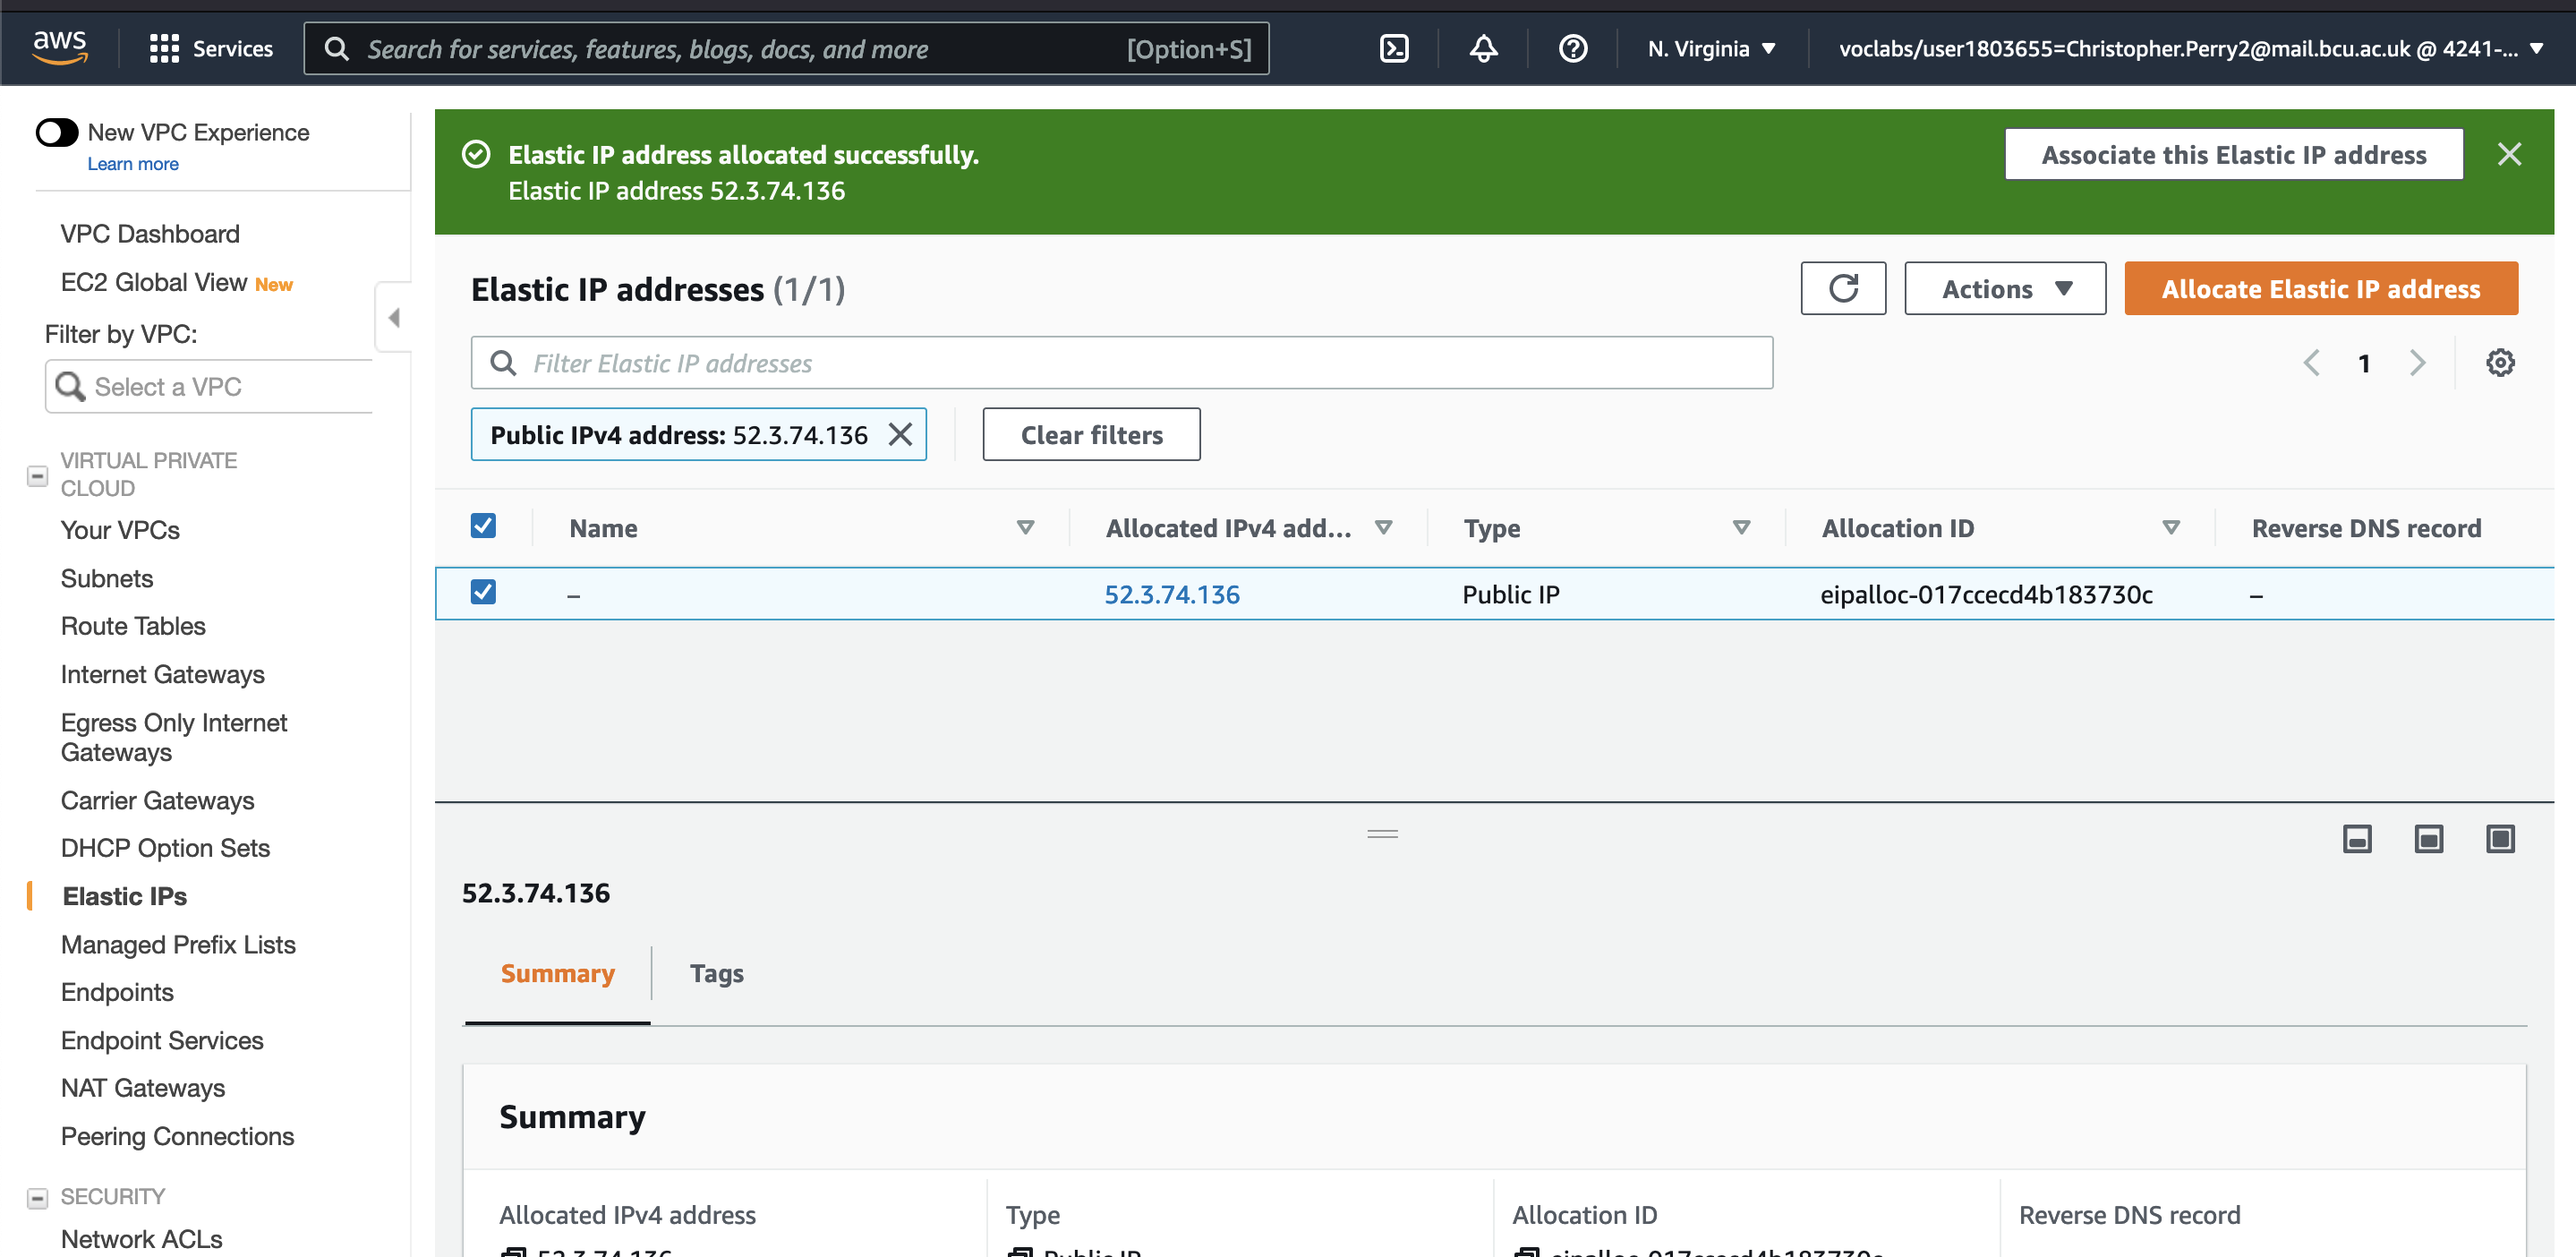
\includegraphics[width=\textwidth]{resources/after-allocate-elastic-ip-address.png}
    \caption{After Allocating Elastic IP Address}
    \label{fig:after-allocate-elastic-ip-address}
\end{figure}


\begin{figure}[H]
    \centering
        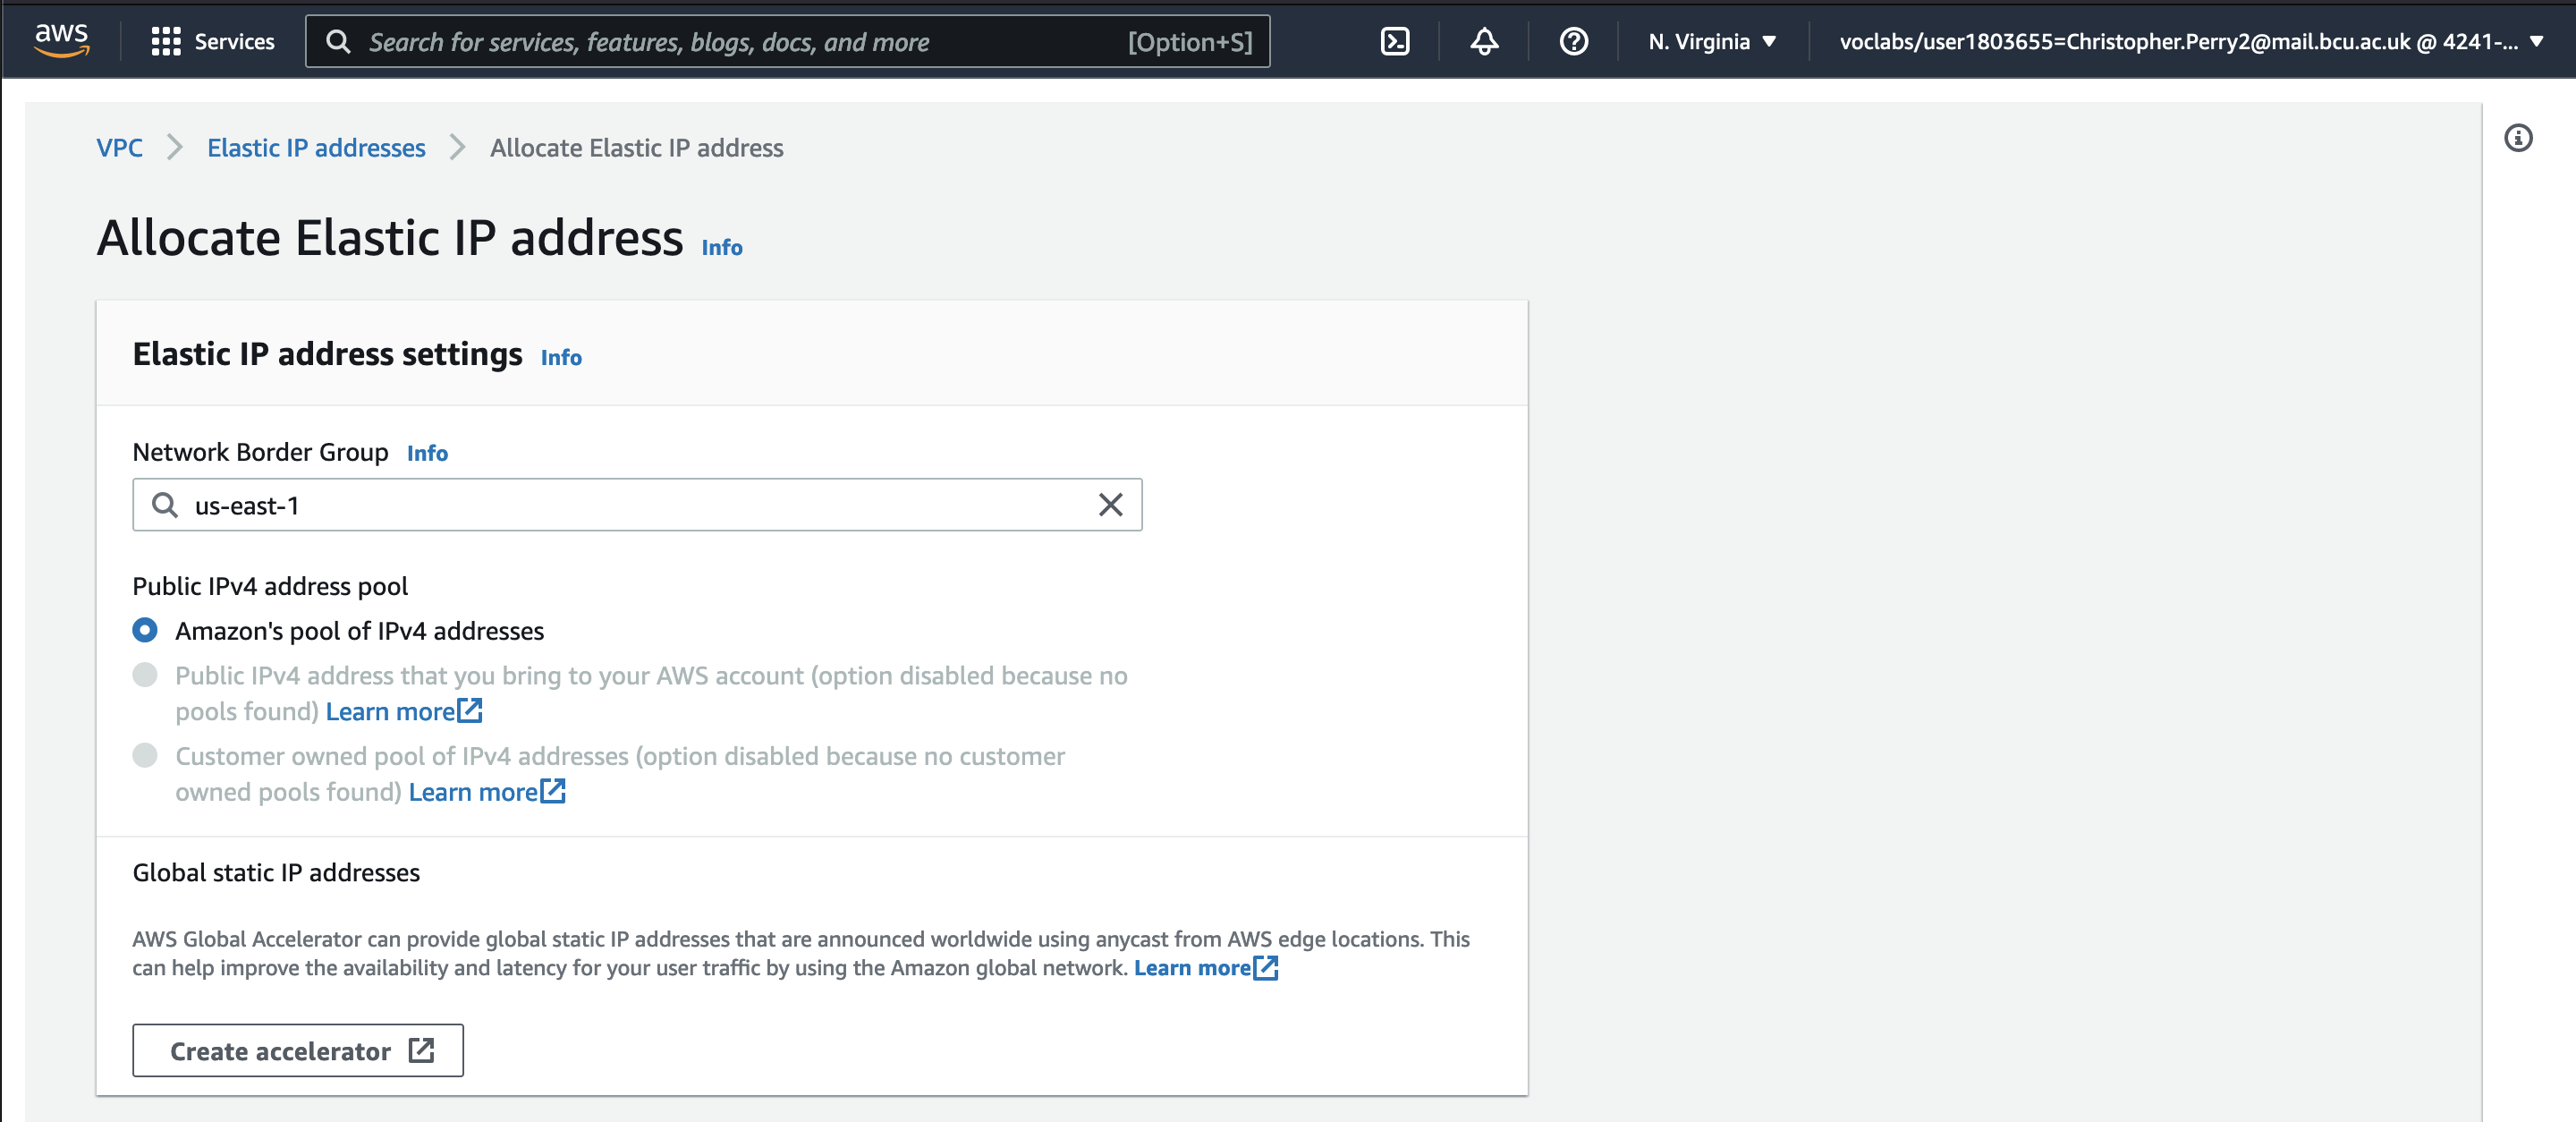
\includegraphics[width=\textwidth]{resources/allocate-elastic-ip-address.png}
    \caption{Allocating Elastic IP Address}
    \label{fig:allocate-elastic-ip-address}
\end{figure}


\begin{figure}[H]
    \centering
        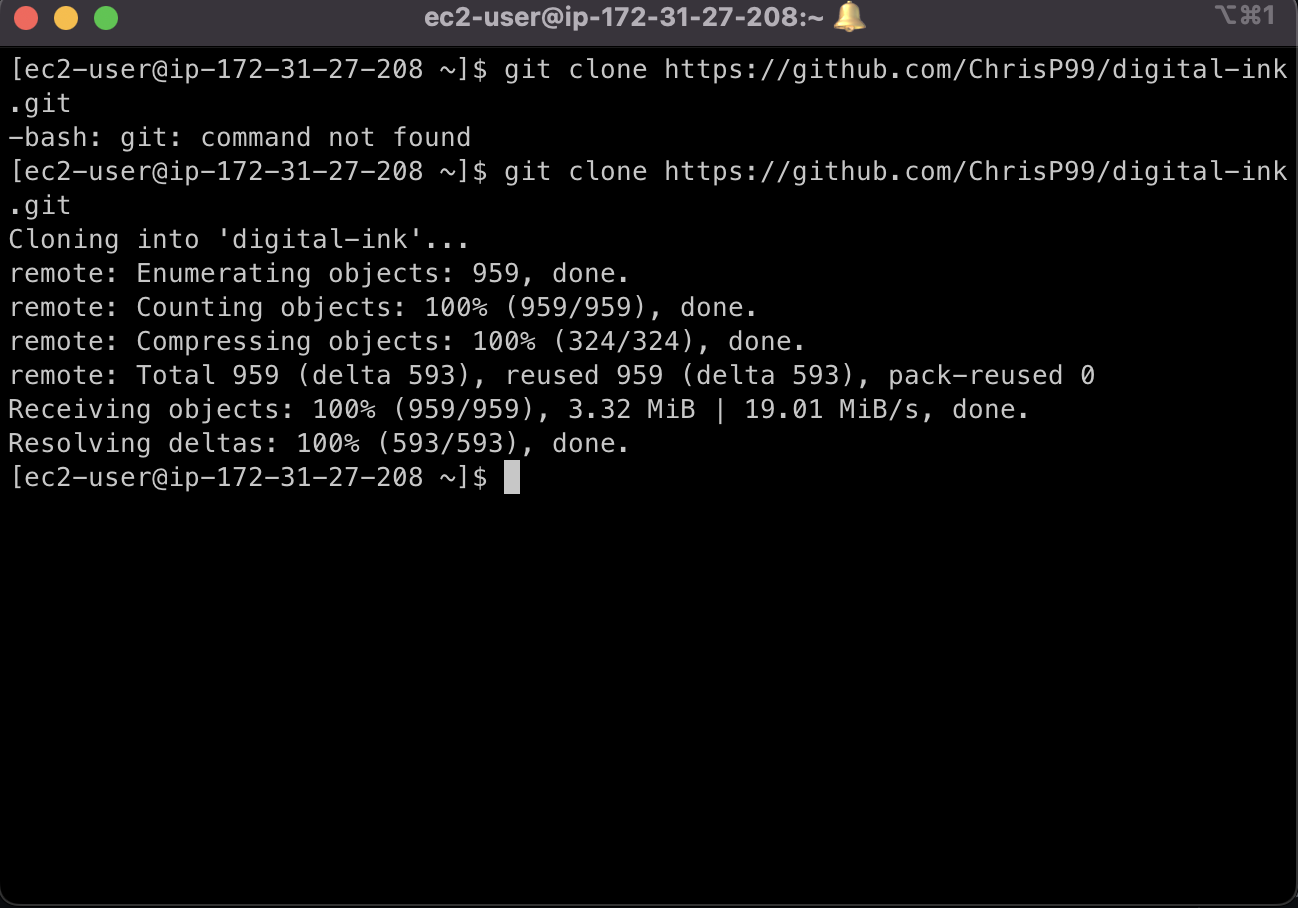
\includegraphics[width=\textwidth]{resources/cloning-the-app.png}
    \caption{Cloning the App}
    \label{fig:cloning-the-app}
\end{figure}

\begin{figure}[H]
    \centering
        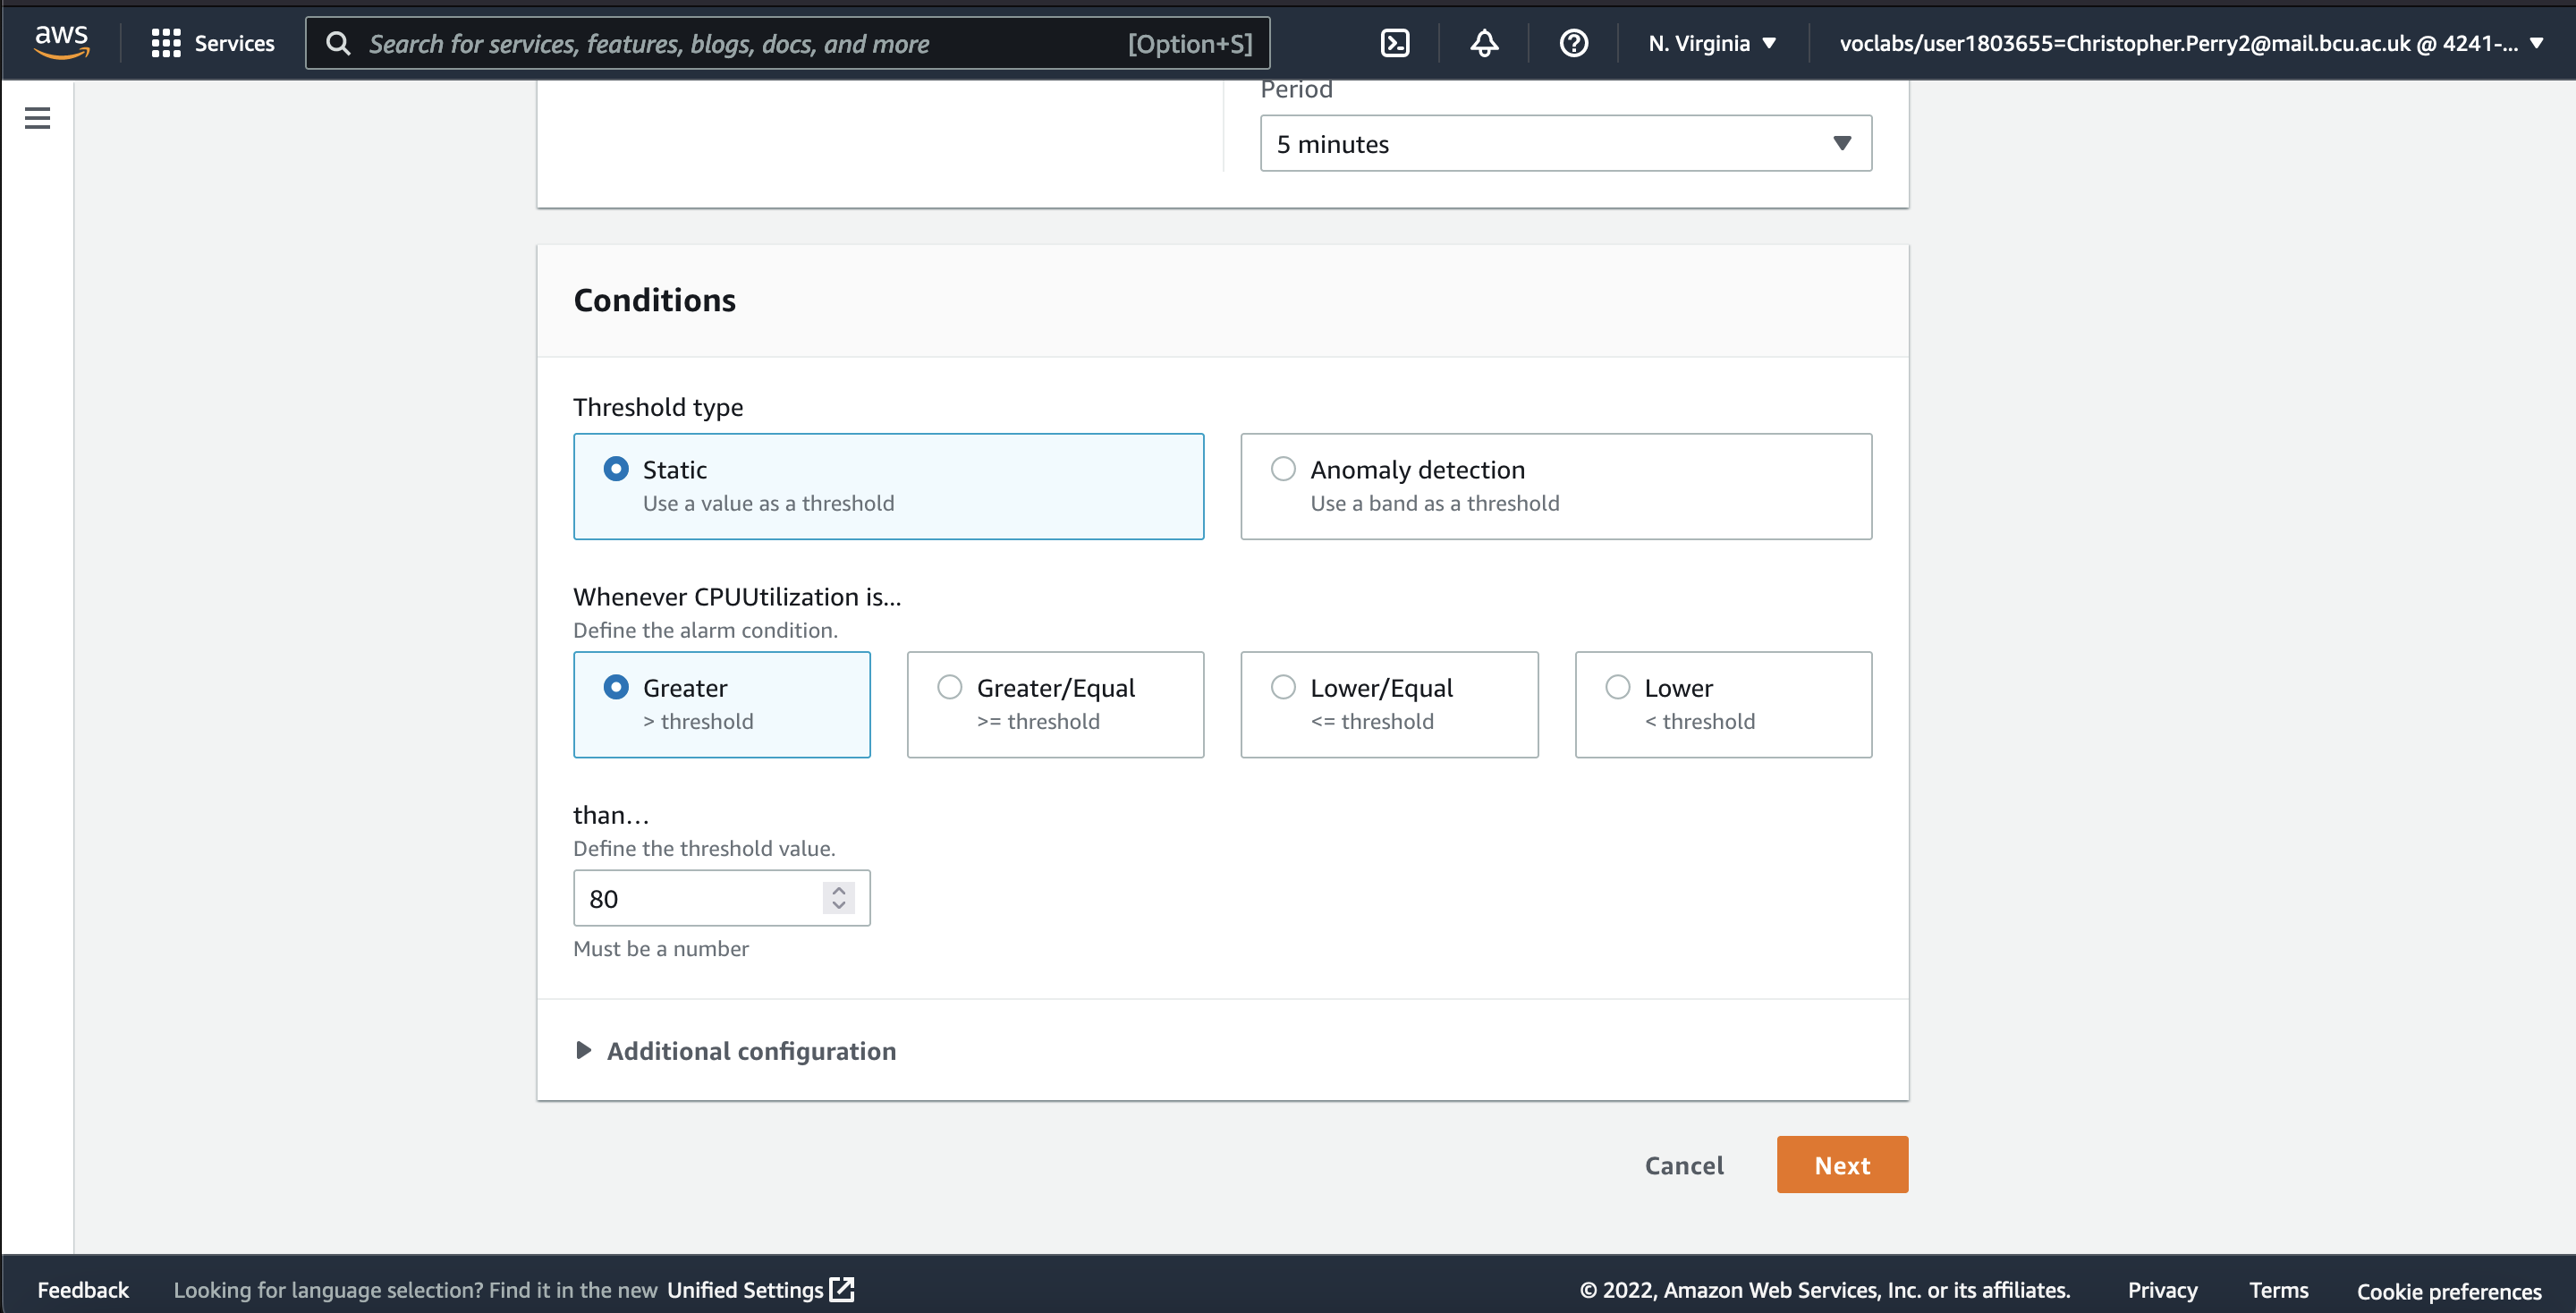
\includegraphics[width=\textwidth]{resources/cloudwatch-conditions.png}
    \caption{CloudWatch Conditions}
    \label{fig:cloudwatch-conditions}
\end{figure}

\begin{figure}[H]
    \centering
        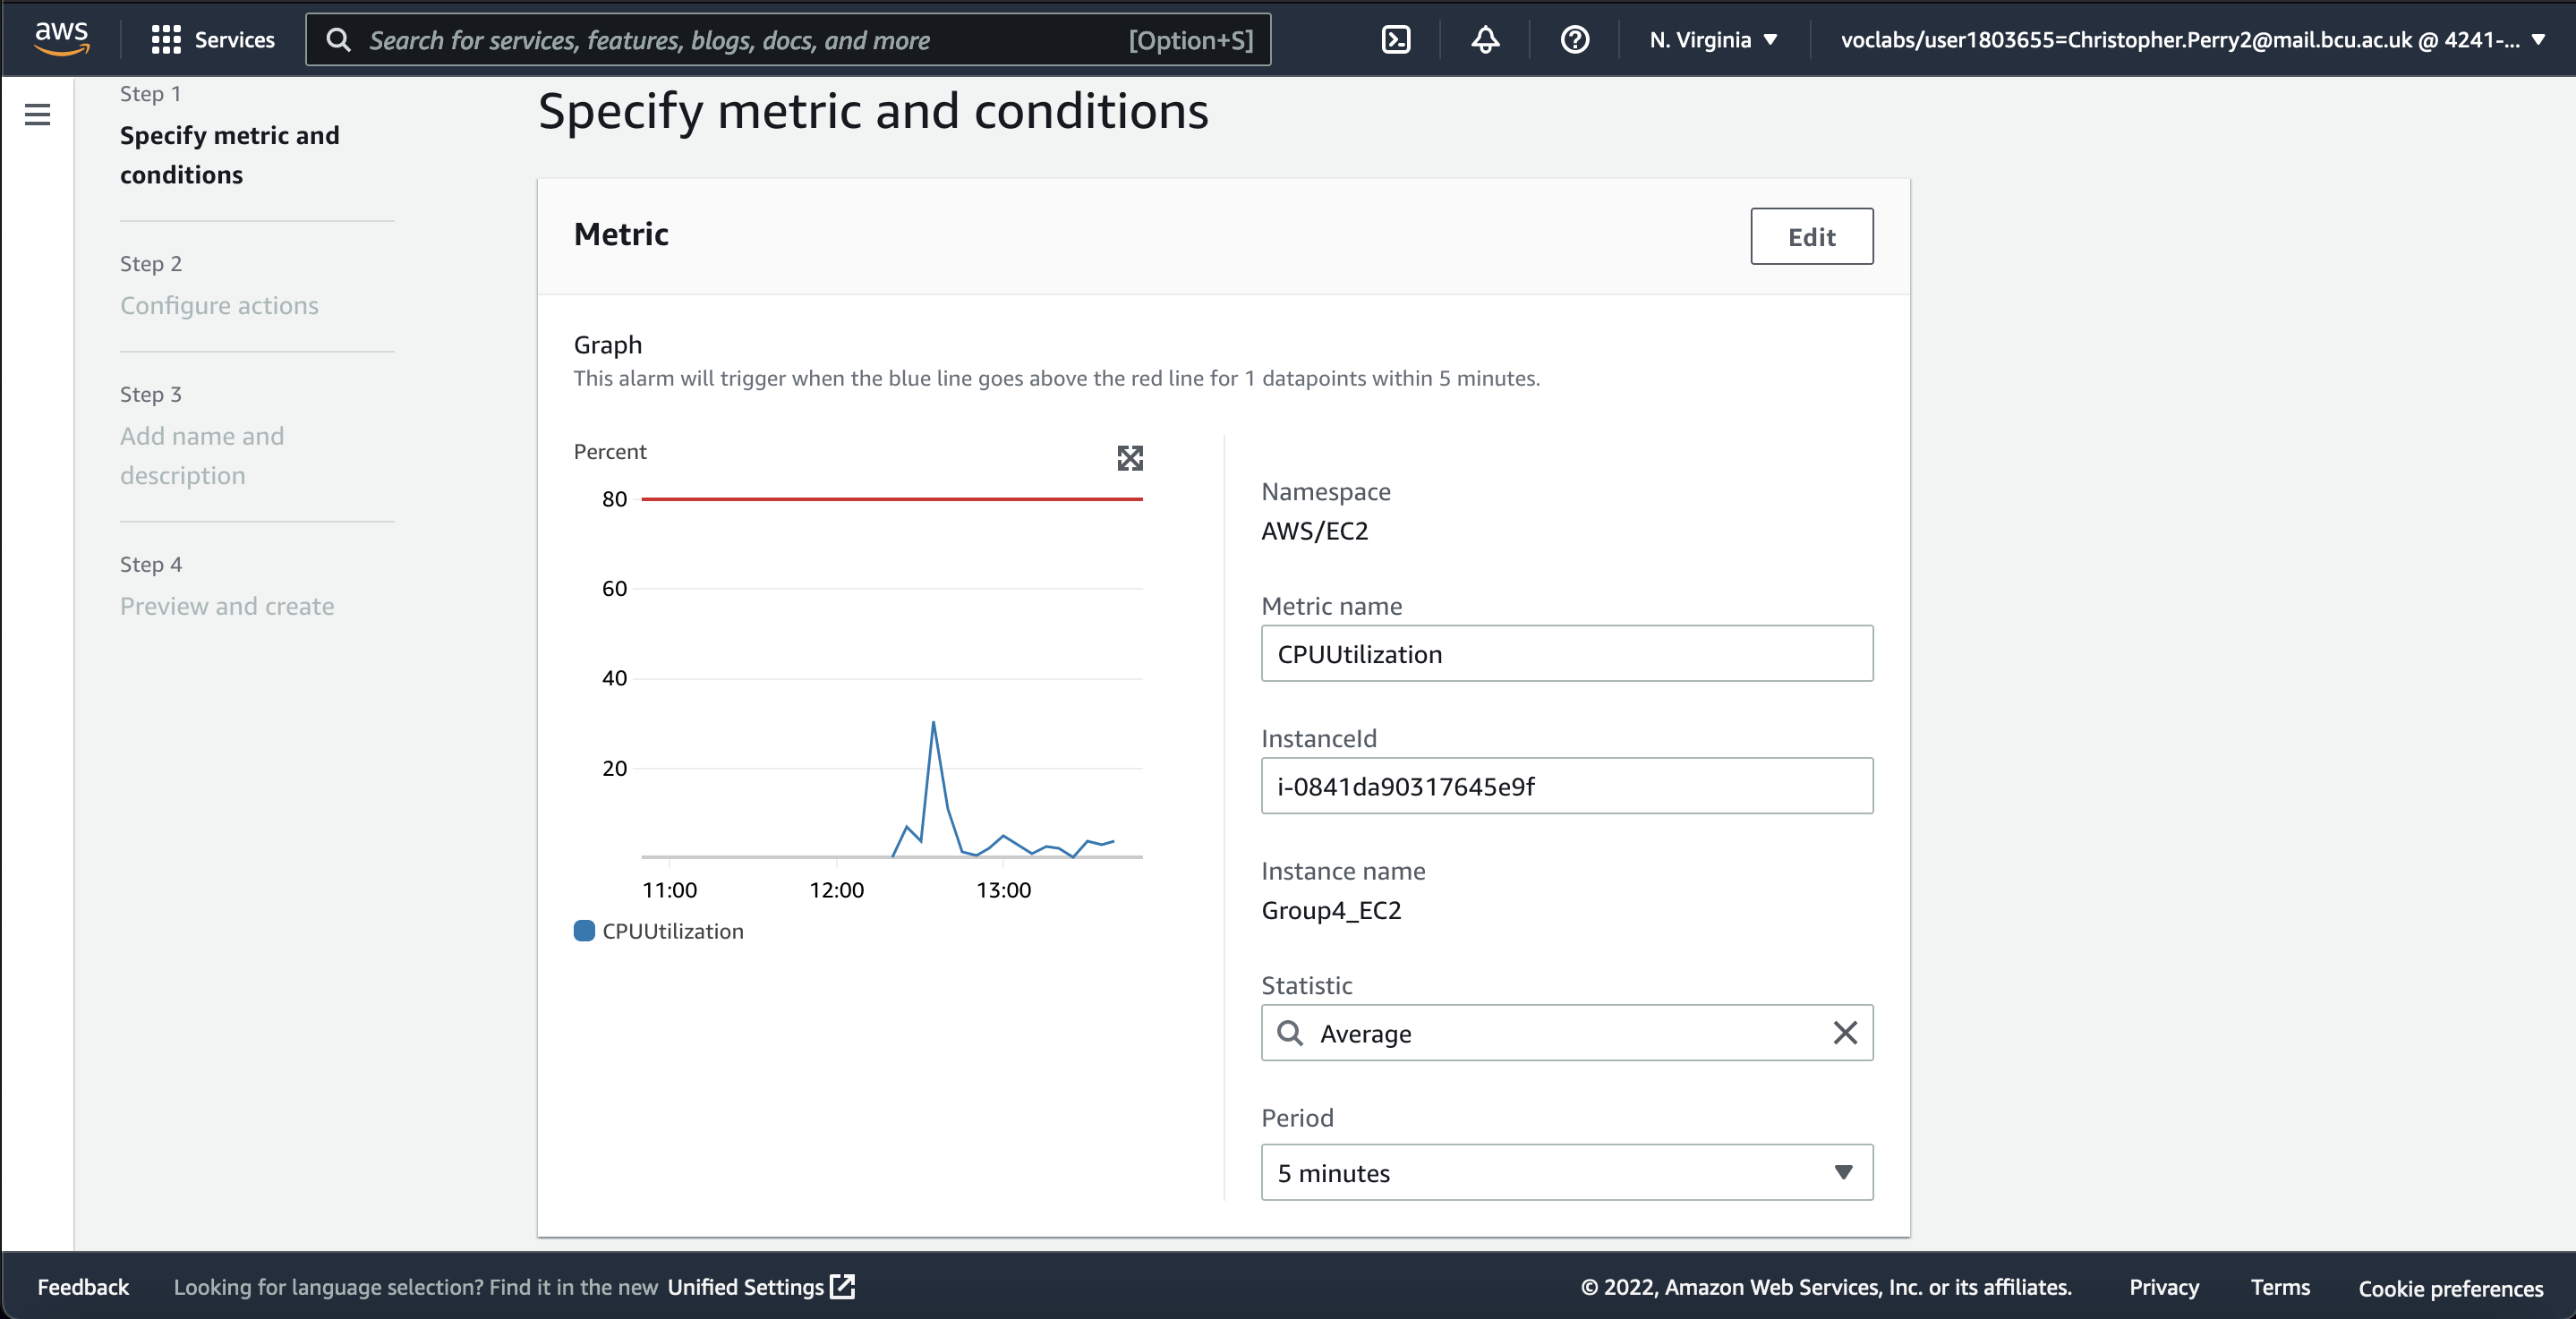
\includegraphics[width=\textwidth]{resources/cloudwatch-specify-metric.png}
    \caption{CloudWatch Specify Metric}
    \label{fig:cloudwatch-specify-metric}
\end{figure}

\begin{figure}[H]
    \centering
        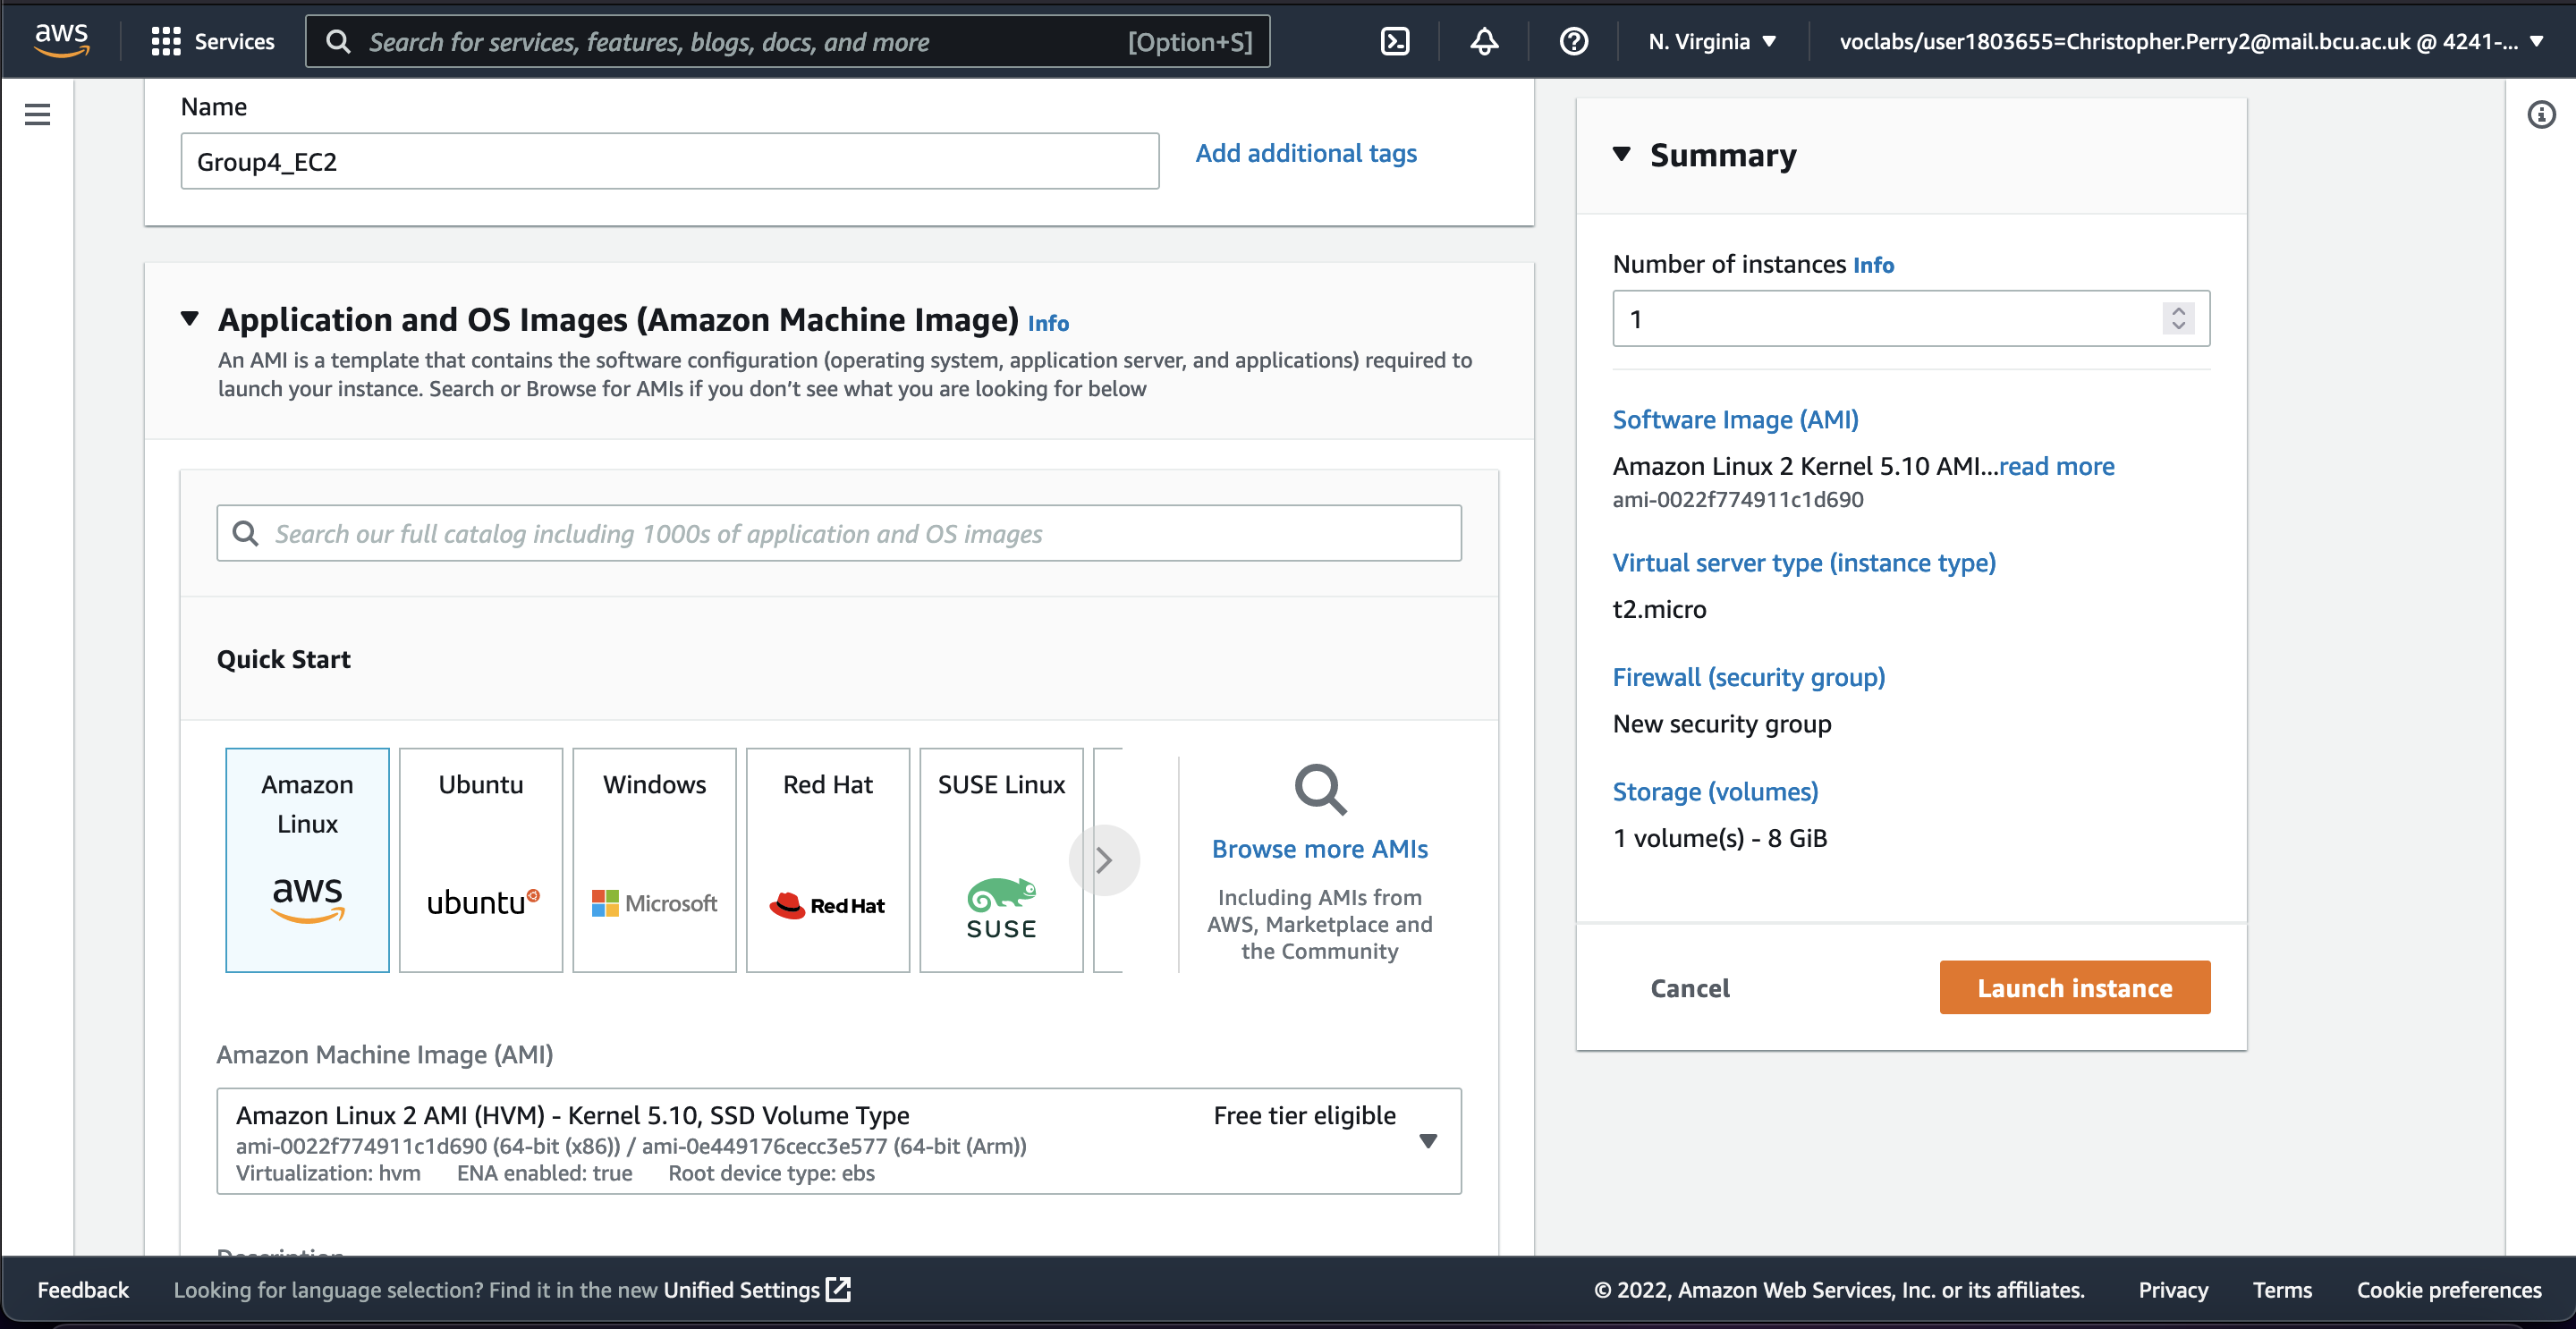
\includegraphics[width=\textwidth]{resources/ec2/create-instance-application-and-os-images}
    \caption{Create Instance - Application and OS Images}
    \label{fig:create-instance-application-and-os-images}
\end{figure}

\begin{figure}[H]
    \centering
        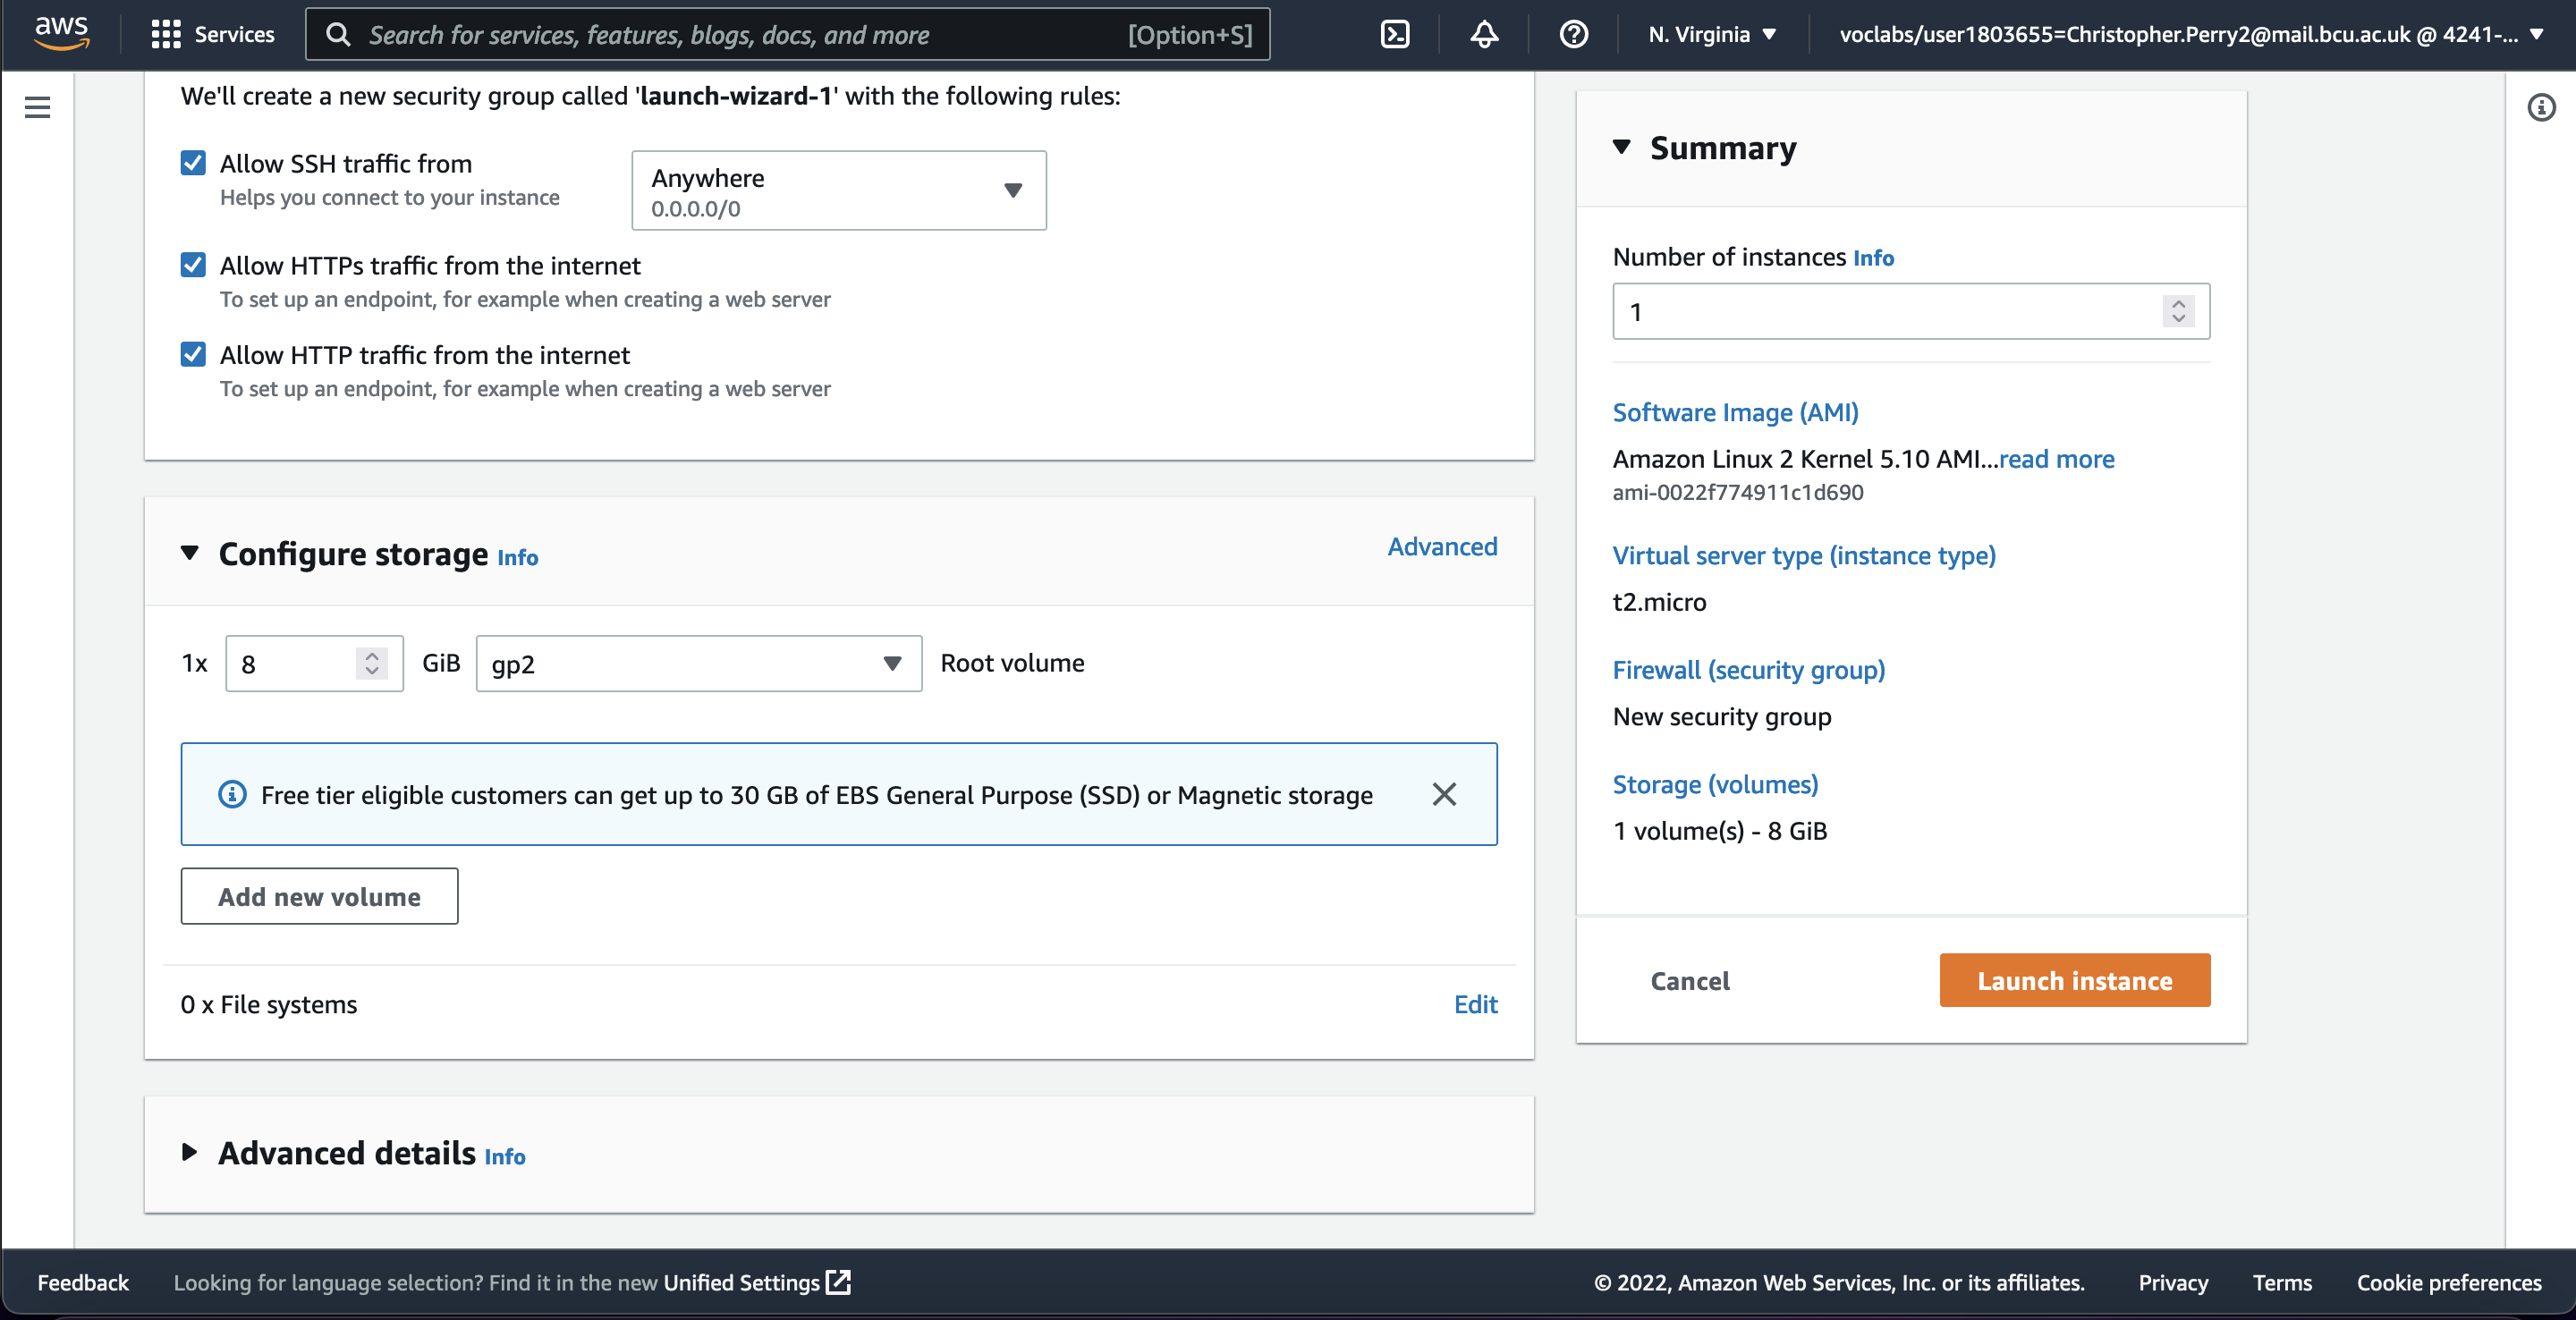
\includegraphics[width=\textwidth]{resources/ec2/create-instance-configure-storage}
    \caption{Create Instance - Configure Storage}
    \label{fig:create-instance-configure-storage}
\end{figure}

\begin{figure}[H]
    \centering
        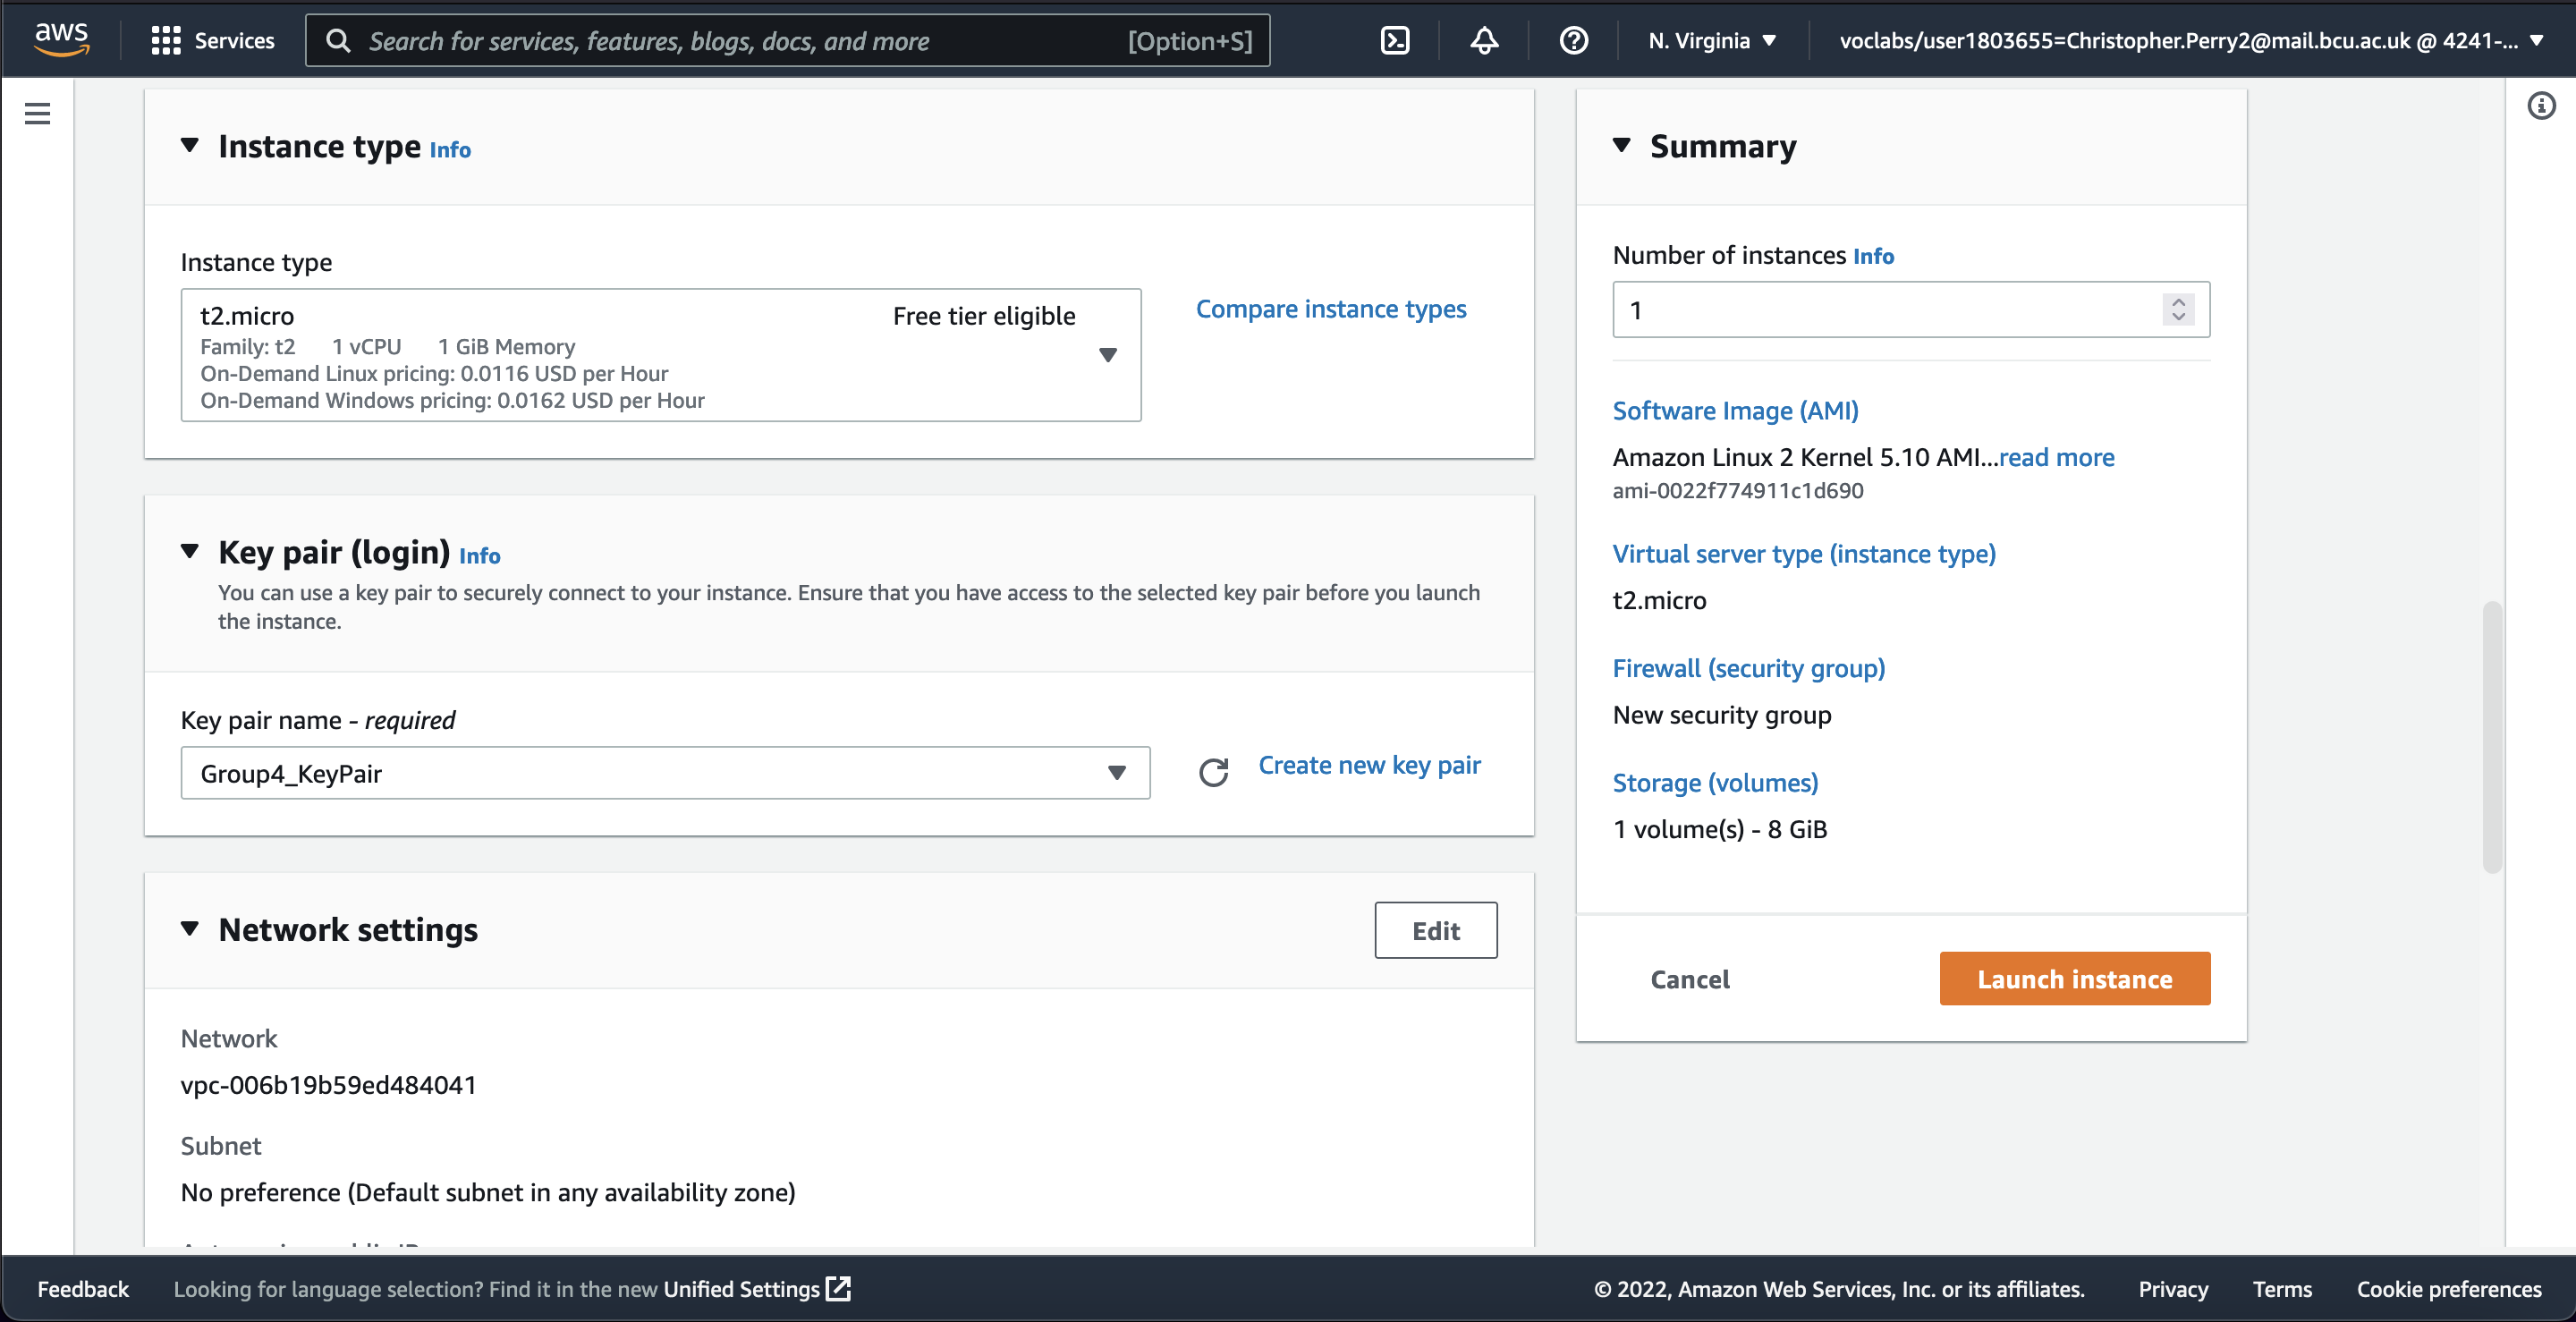
\includegraphics[width=\textwidth]{resources/ec2/create-instance-instance-type}
    \caption{Create Instance - Instance Type}
    \label{fig:create-instance-instance-type}
\end{figure}

\begin{figure}[H]
    \centering
        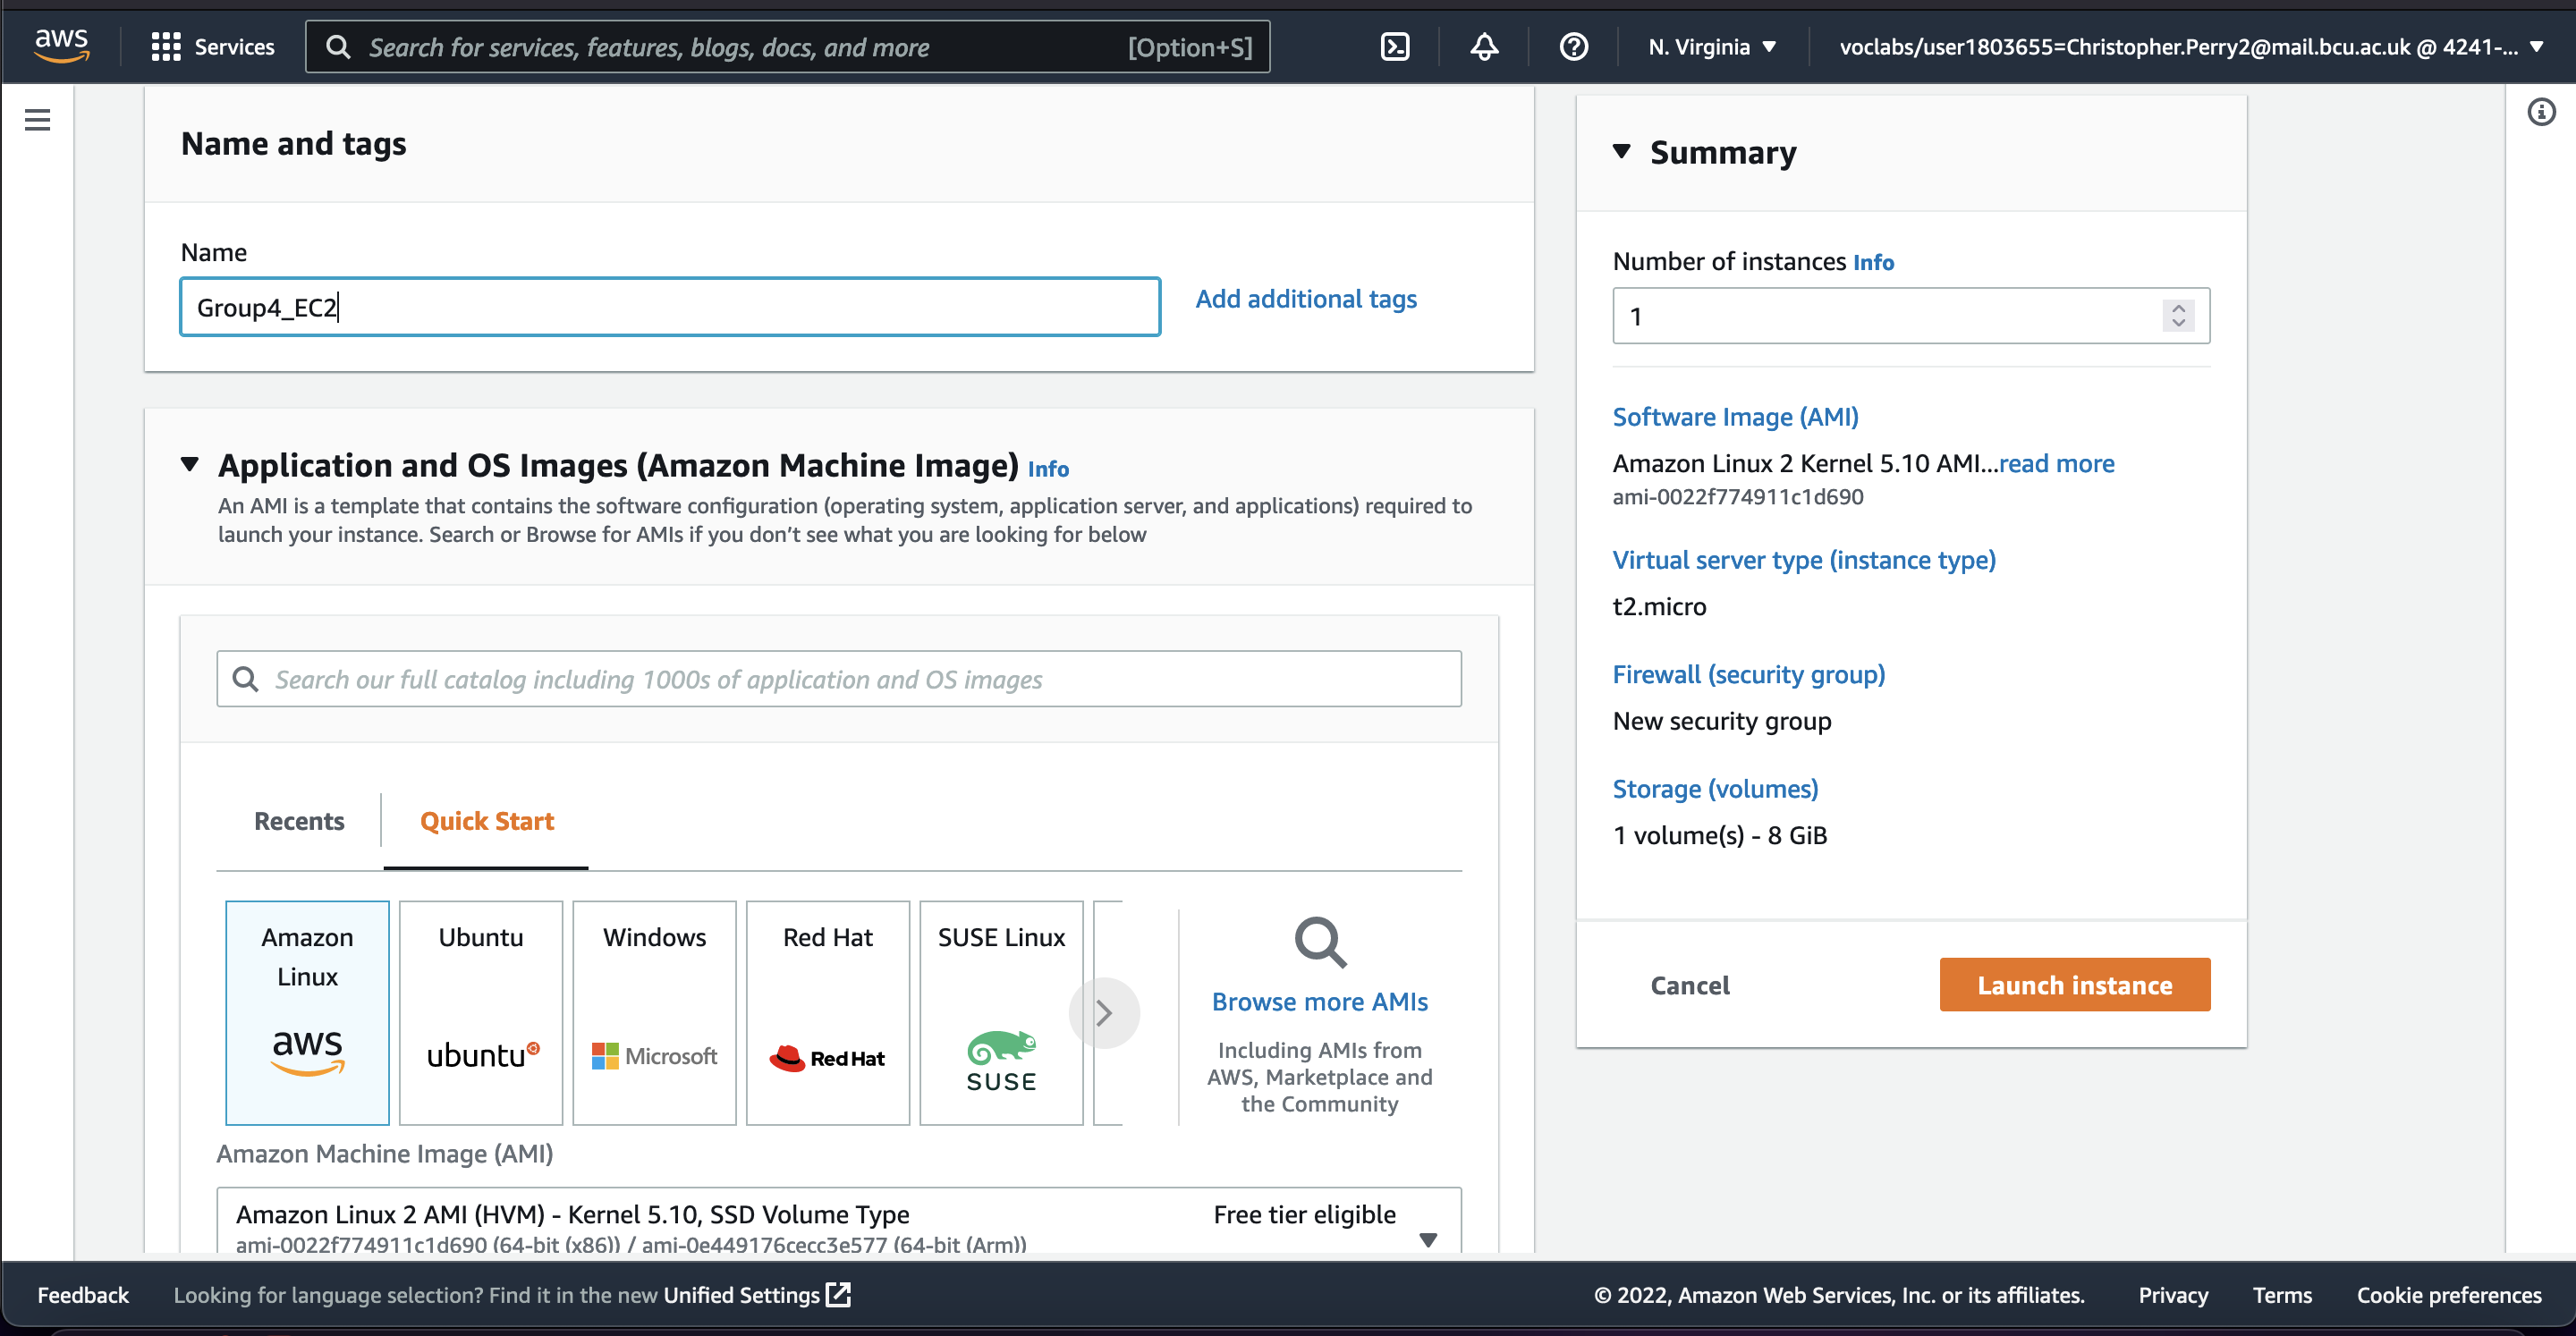
\includegraphics[width=\textwidth]{resources/ec2/create-instance-name-and-tags}
    \caption{Create Instance - Name \& Tags}
    \label{fig:create-instance-name-and-tags}
\end{figure}

\begin{figure}[H]
    \centering
        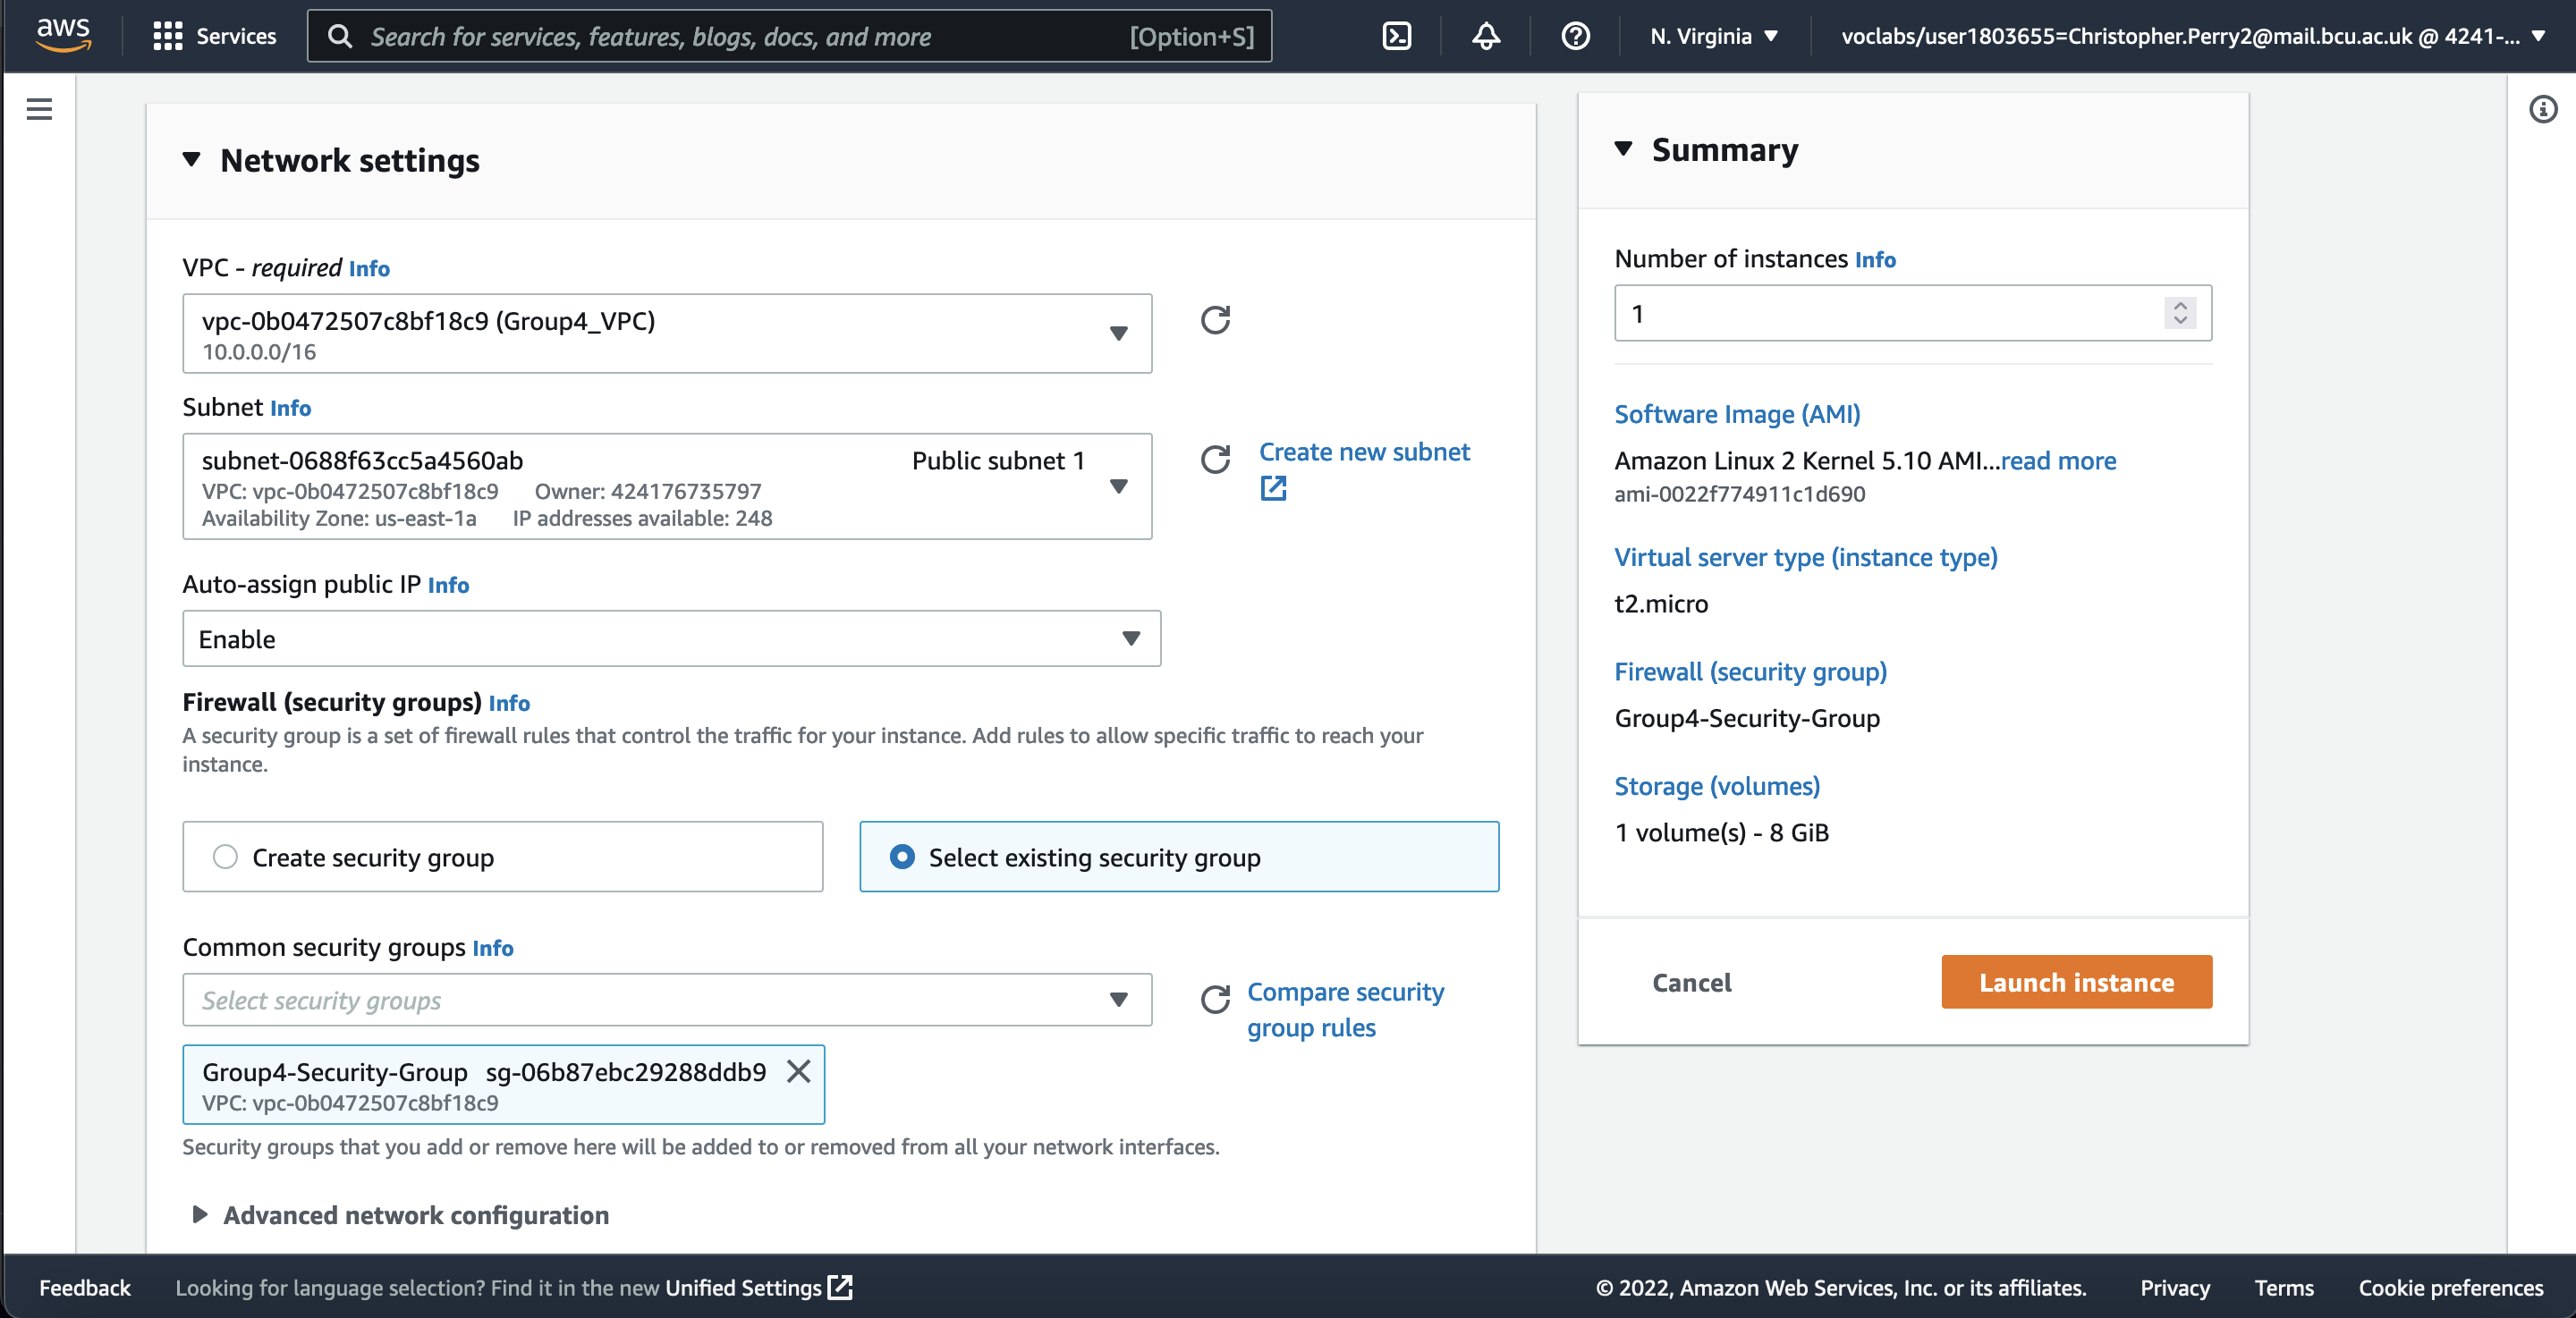
\includegraphics[width=\textwidth]{resources/ec2/create-instance-network-settings}
    \caption{Create Instance - Network Settings}
    \label{fig:create-instance-network-settings}
\end{figure}

\begin{figure}[H]
    \centering
        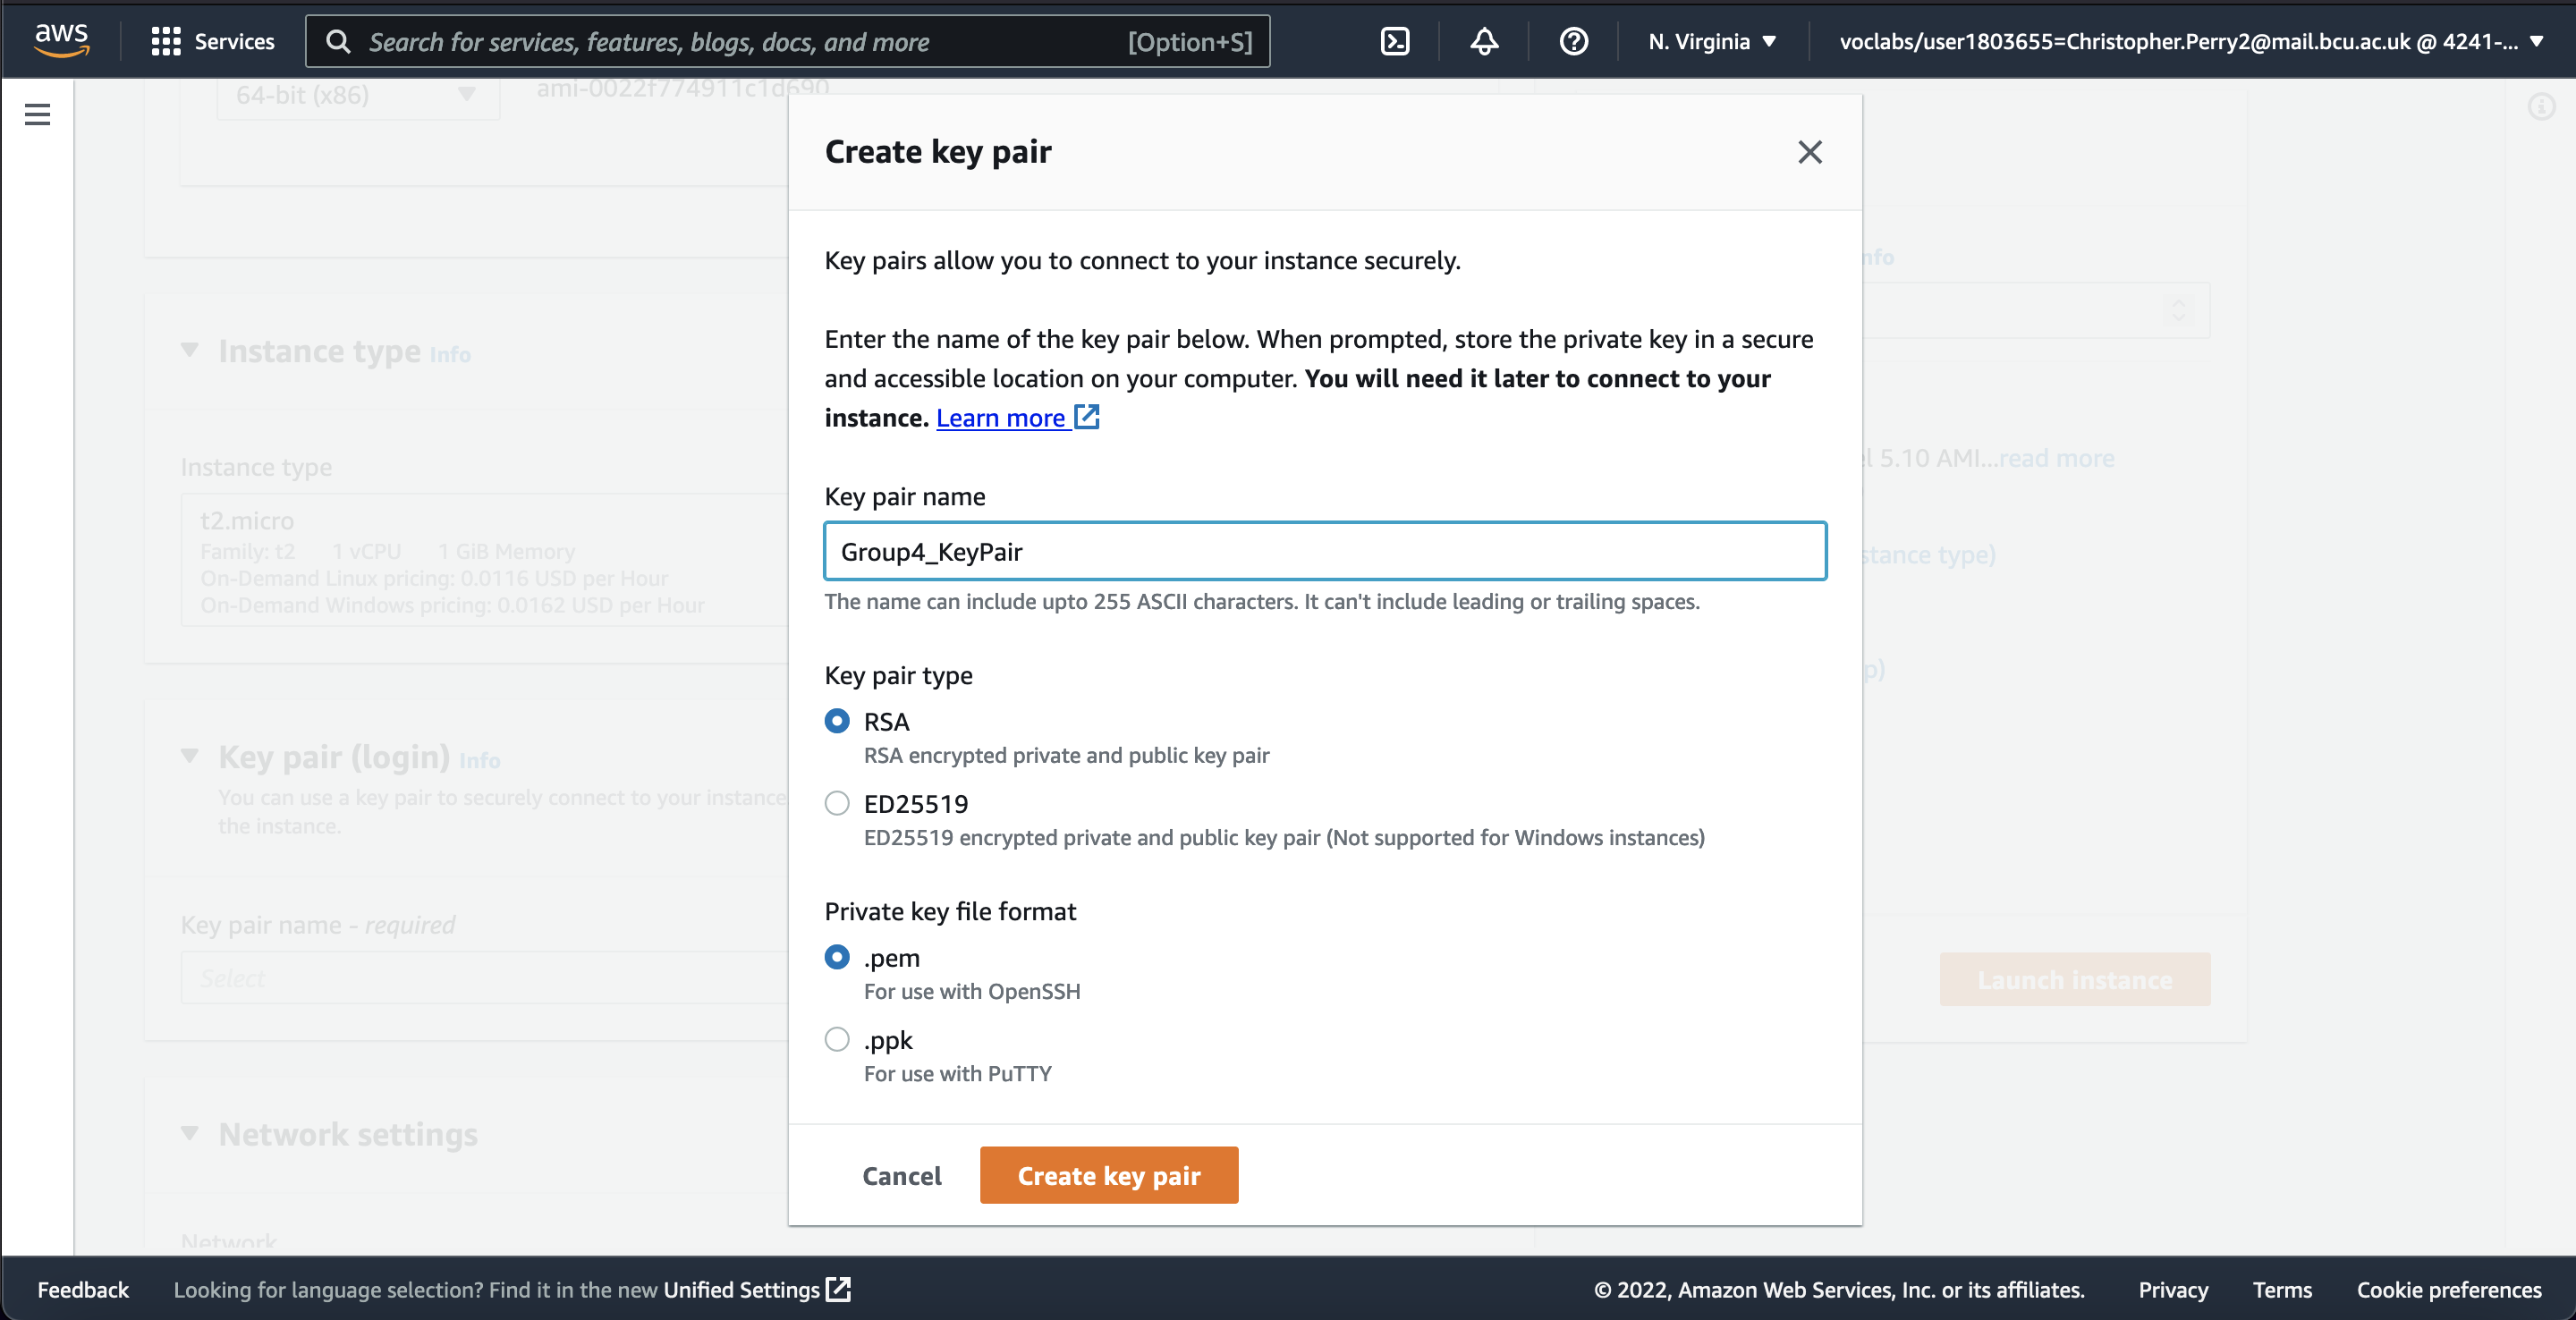
\includegraphics[width=\textwidth]{resources/ec2/create-key-pair}
    \caption{Creating Key Pair}
    \label{fig:create-key-pair}
\end{figure}

\begin{figure}[H]
    \centering
        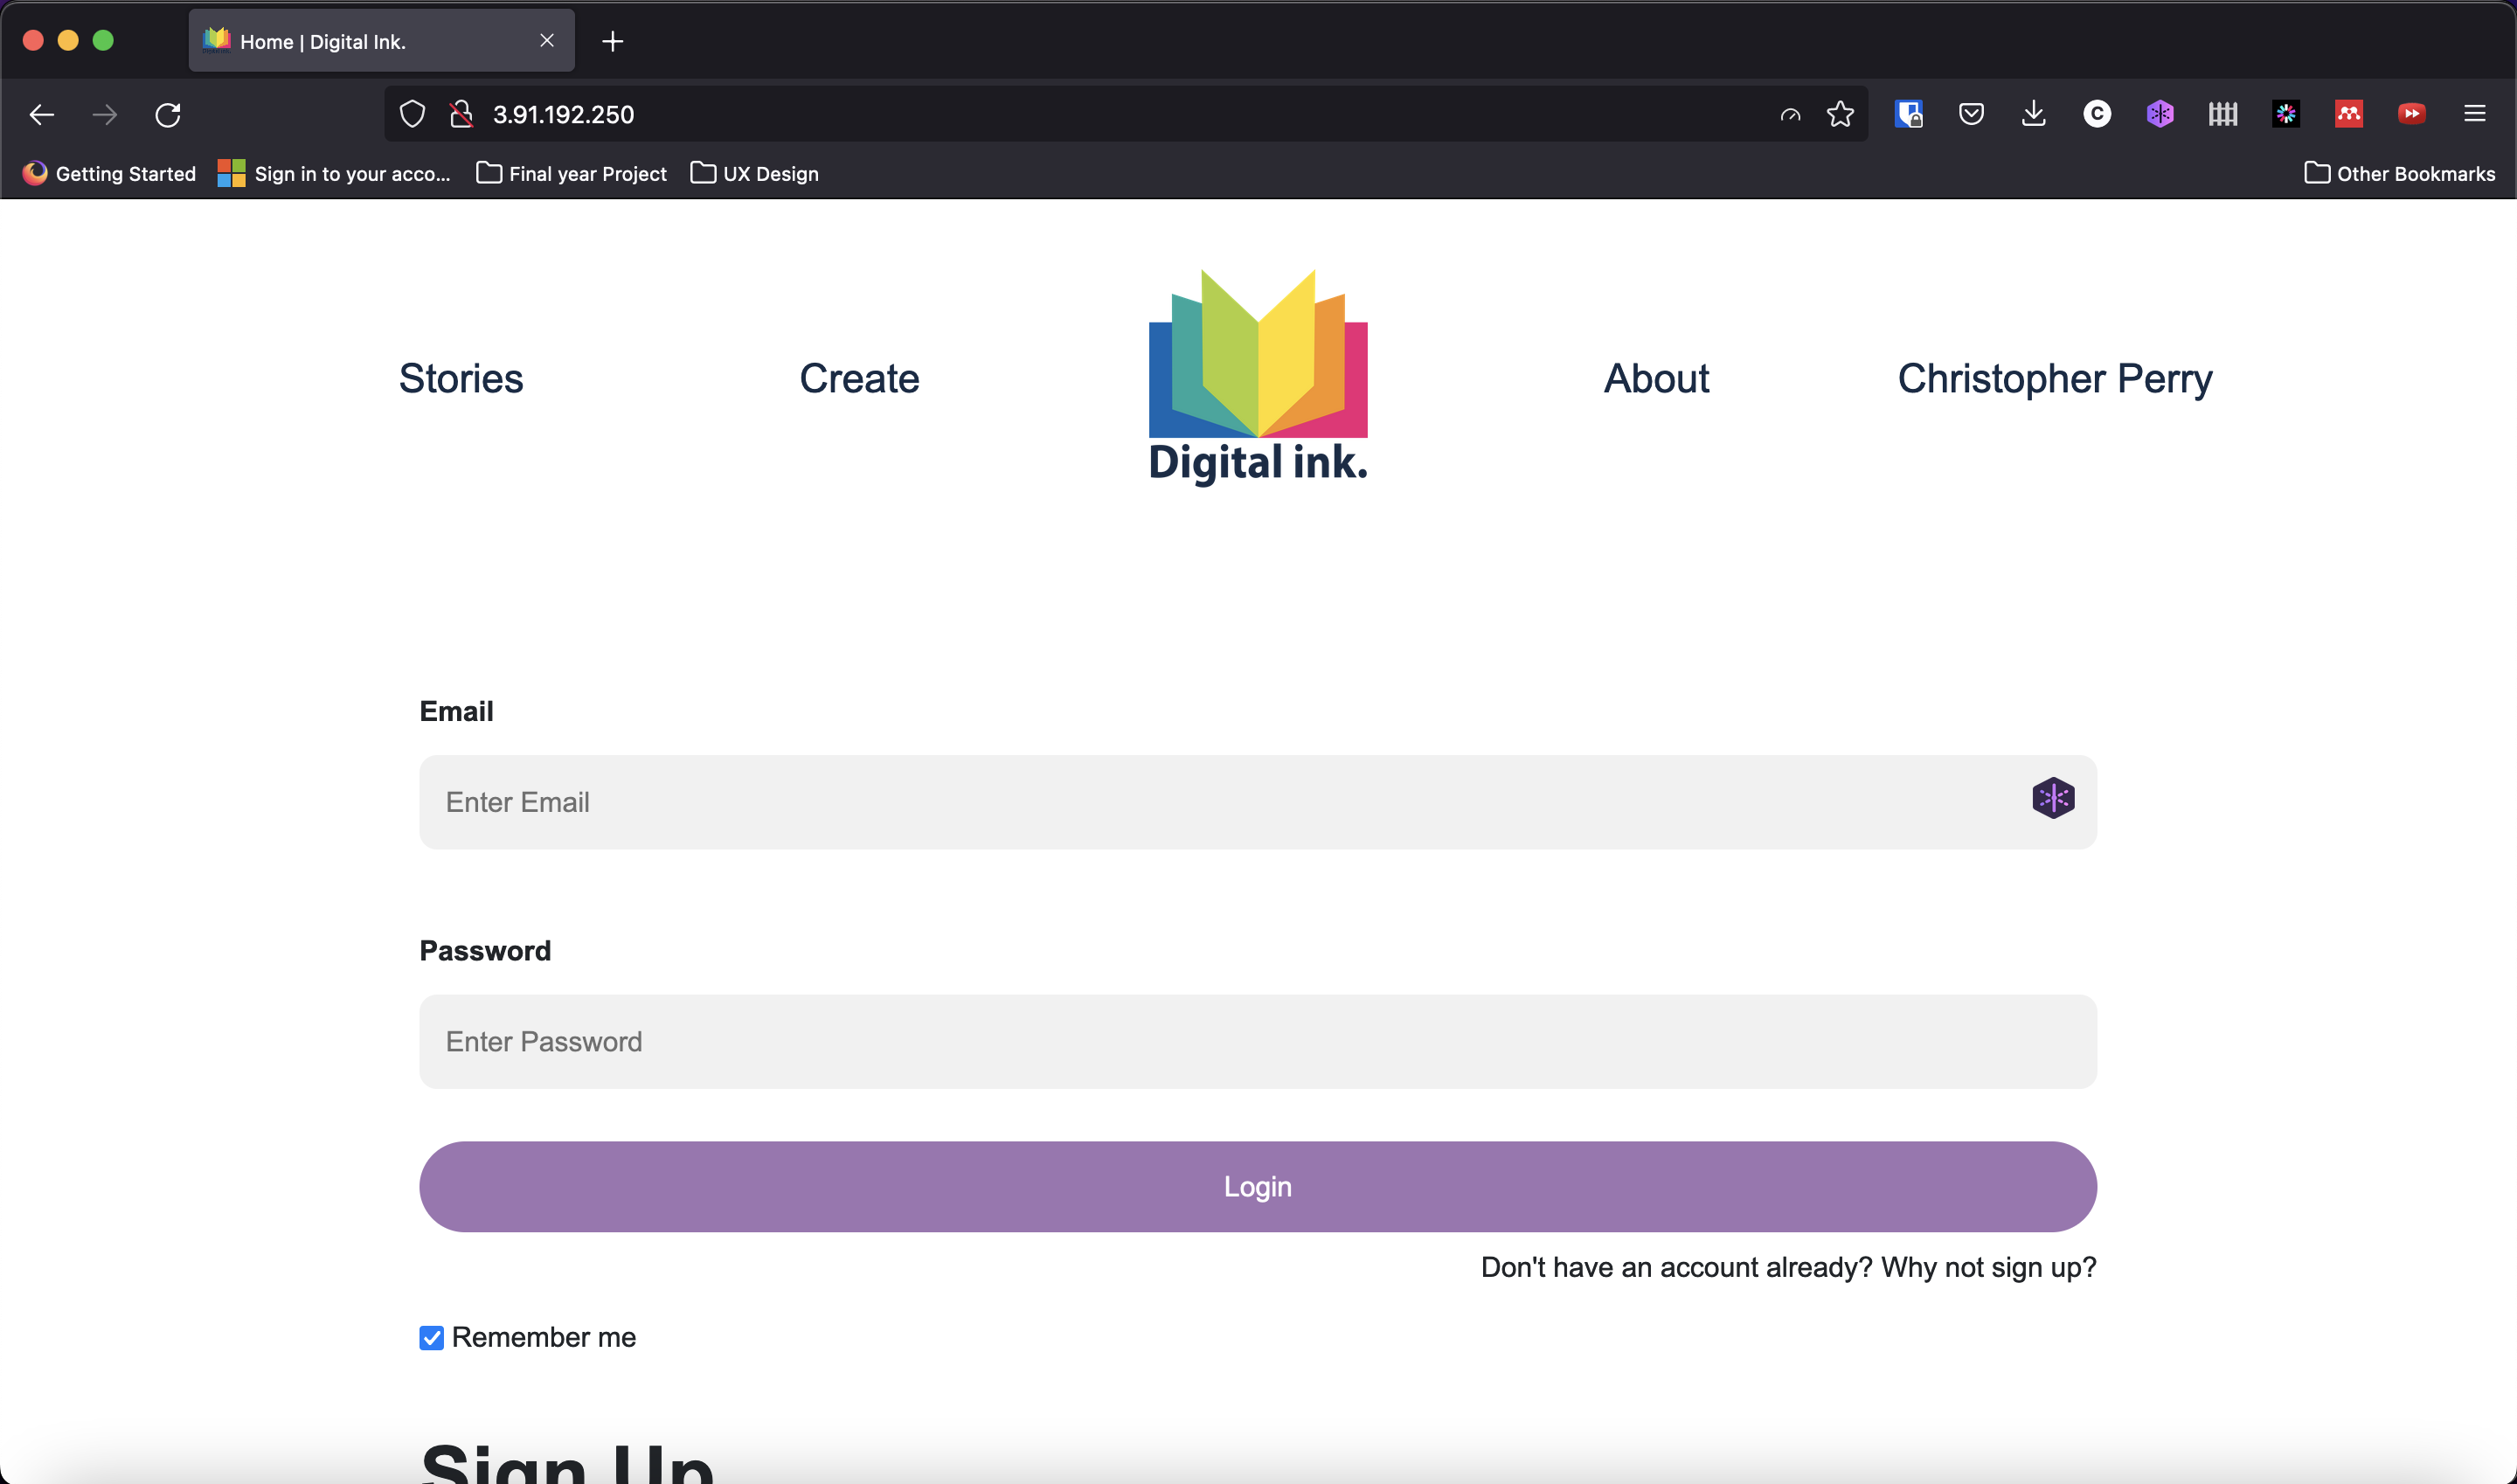
\includegraphics[width=\textwidth]{resources/digital-ink.png}
    \caption{Digital Ink}
    \label{fig:digital-ink}
\end{figure}

\begin{figure}[H]
    \centering
        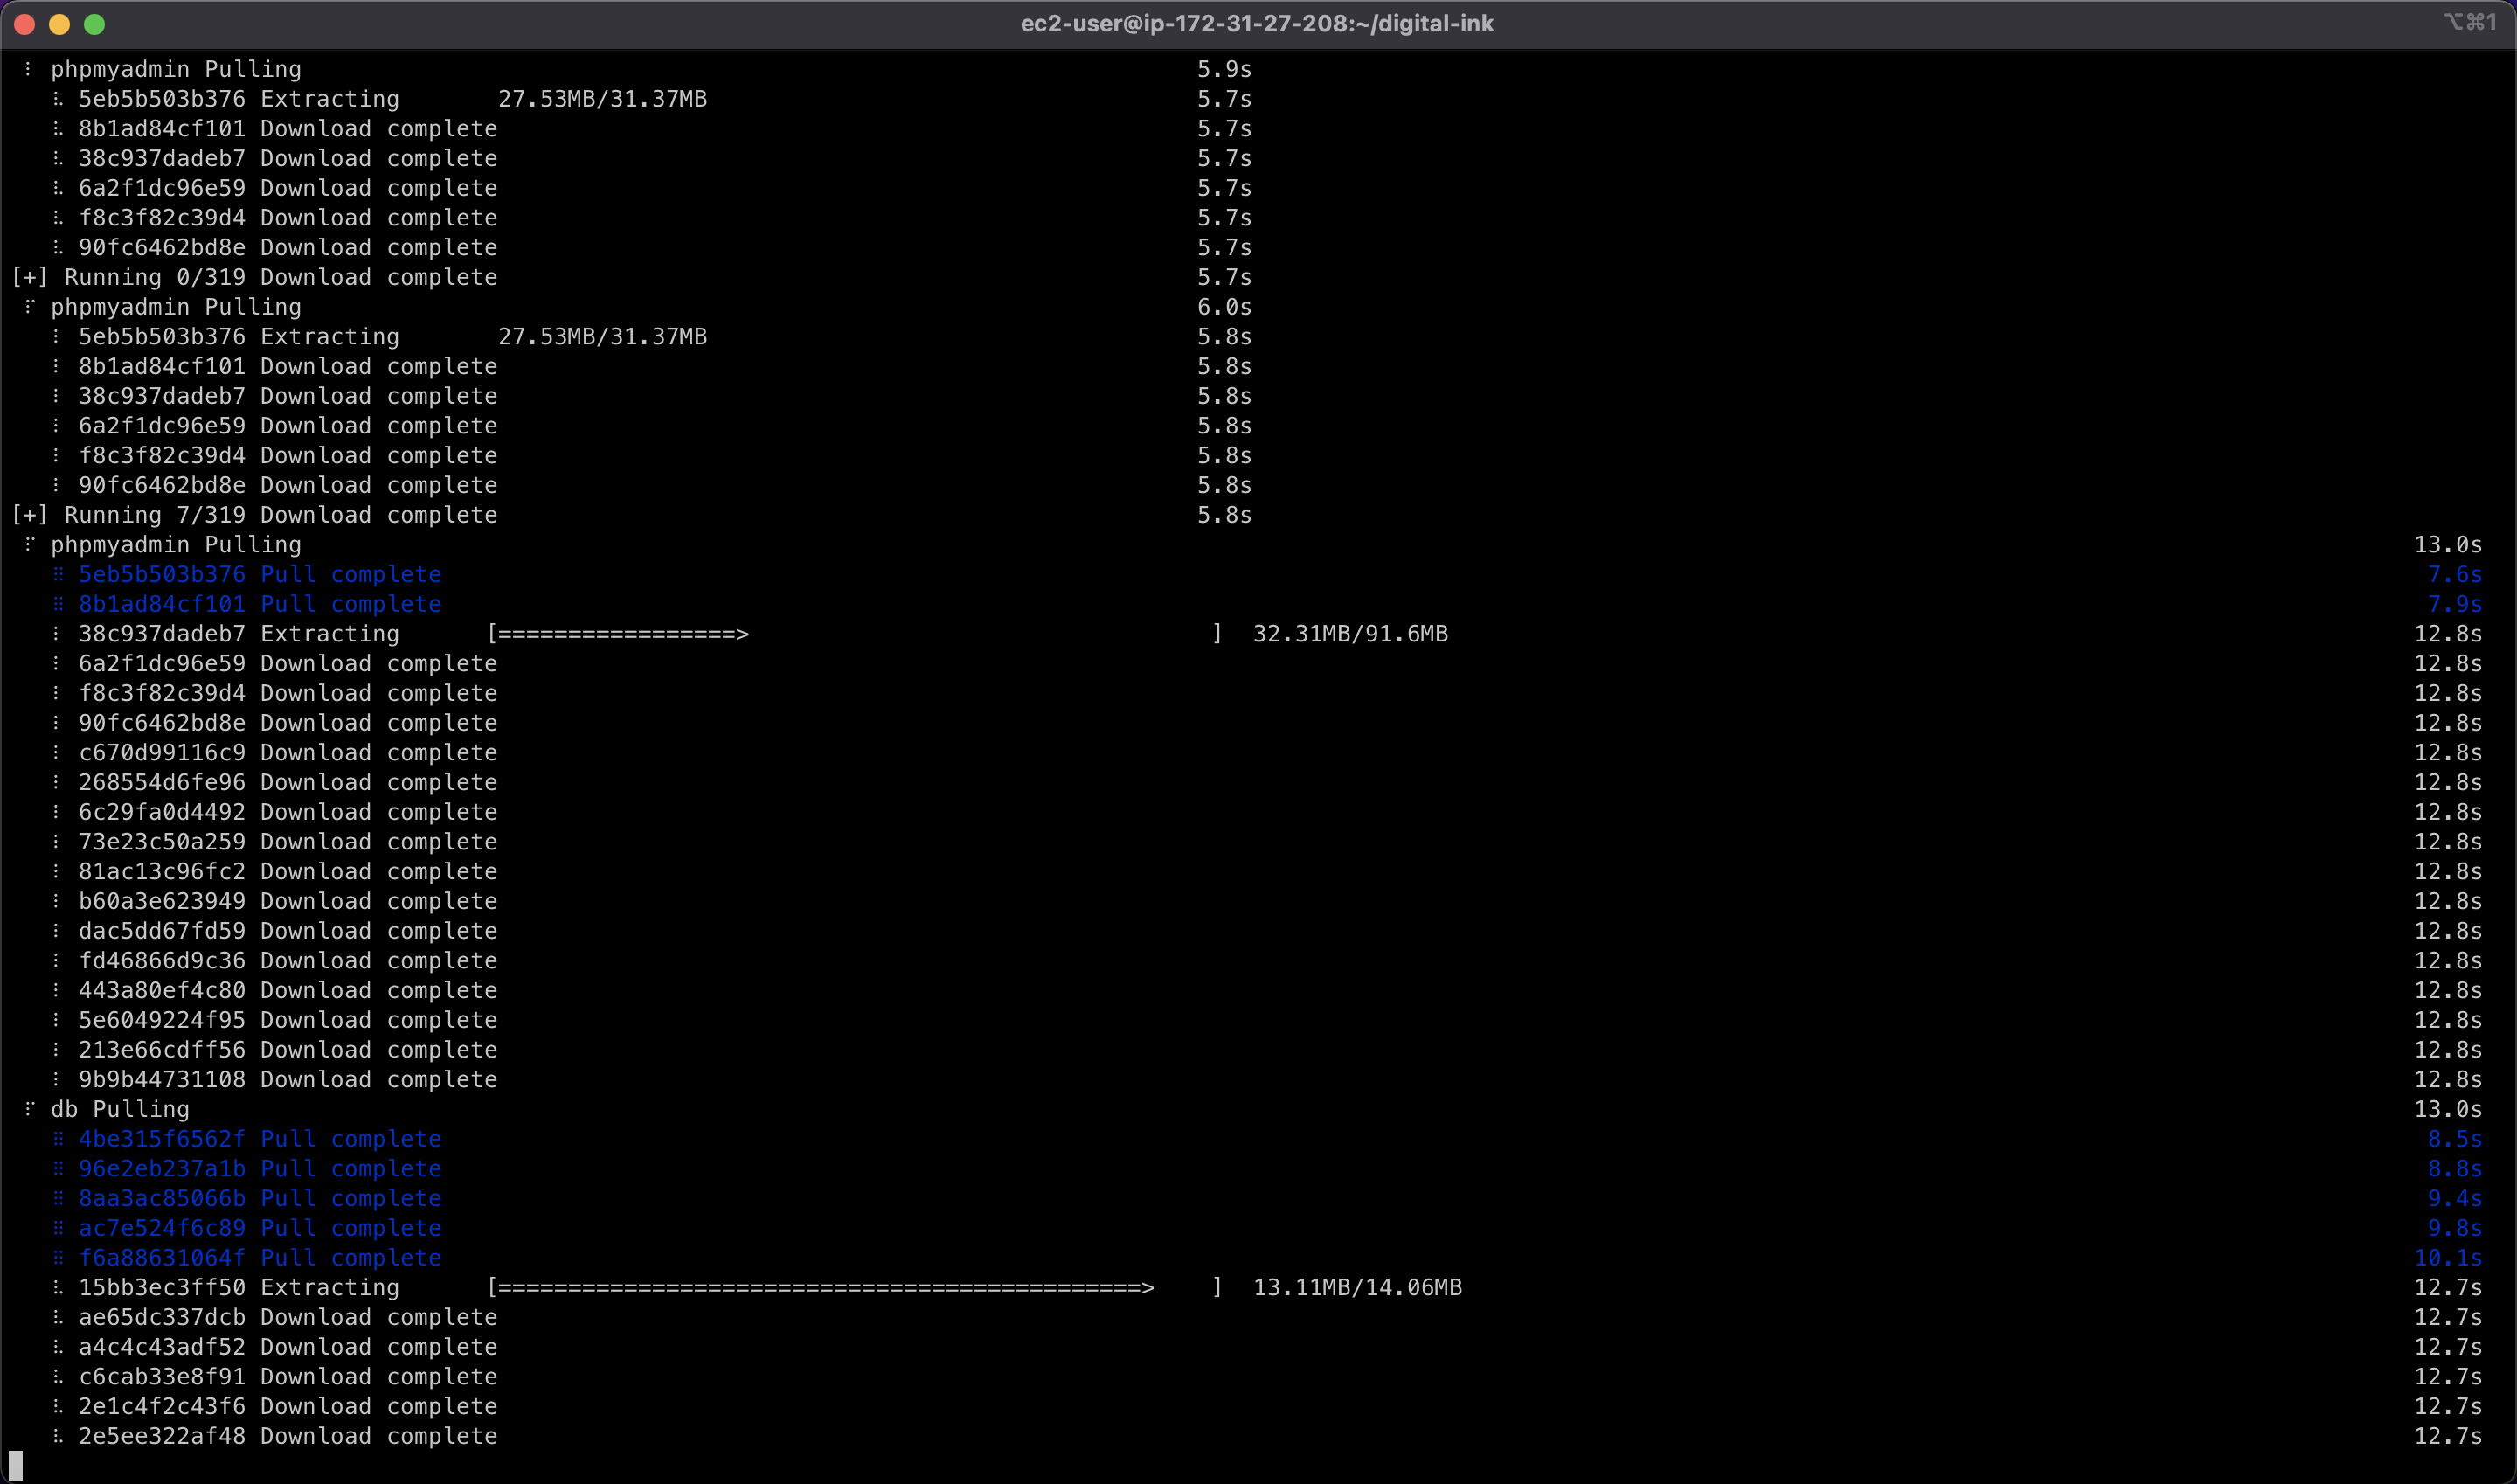
\includegraphics[width=\textwidth]{resources/docker-compose.png}
    \caption{Docker Compose}
    \label{fig:docker-compose}
\end{figure}

\begin{figure}[H]
    \centering
        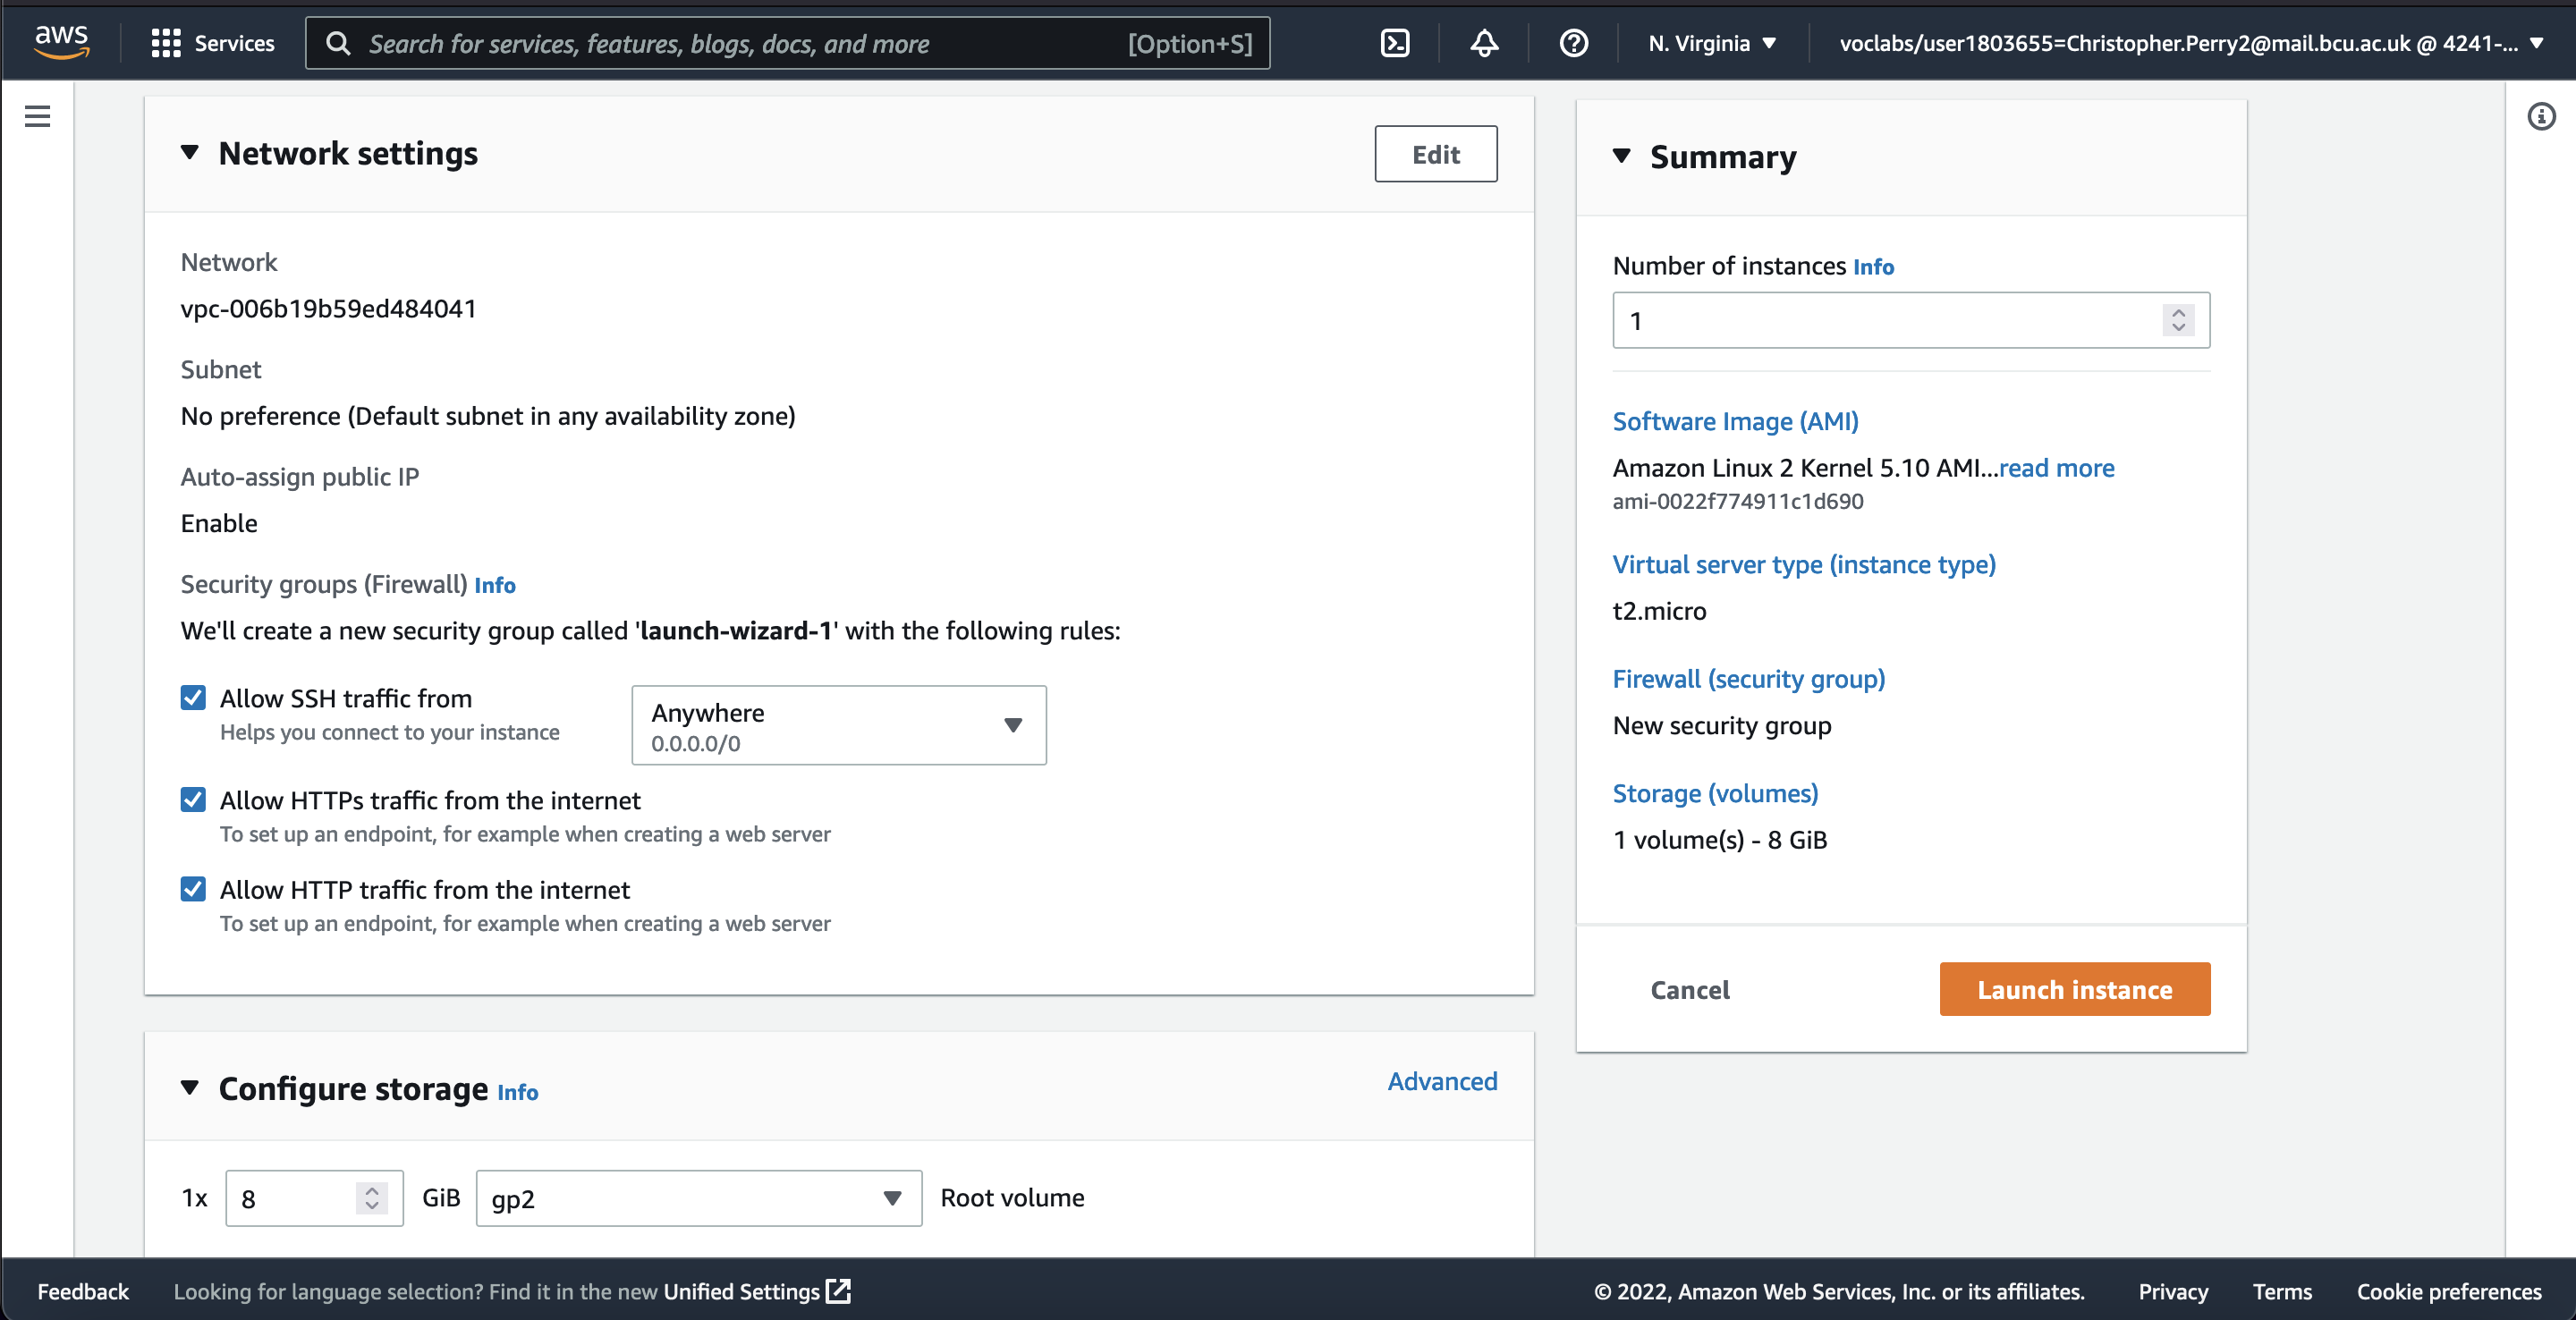
\includegraphics[width=\textwidth]{resources/edit-instance-network-settings.png}
    \caption{Edit Instance - Network Settings}
    \label{fig:edit-instance-network-settings}
\end{figure}

\begin{figure}[H]
    \centering
        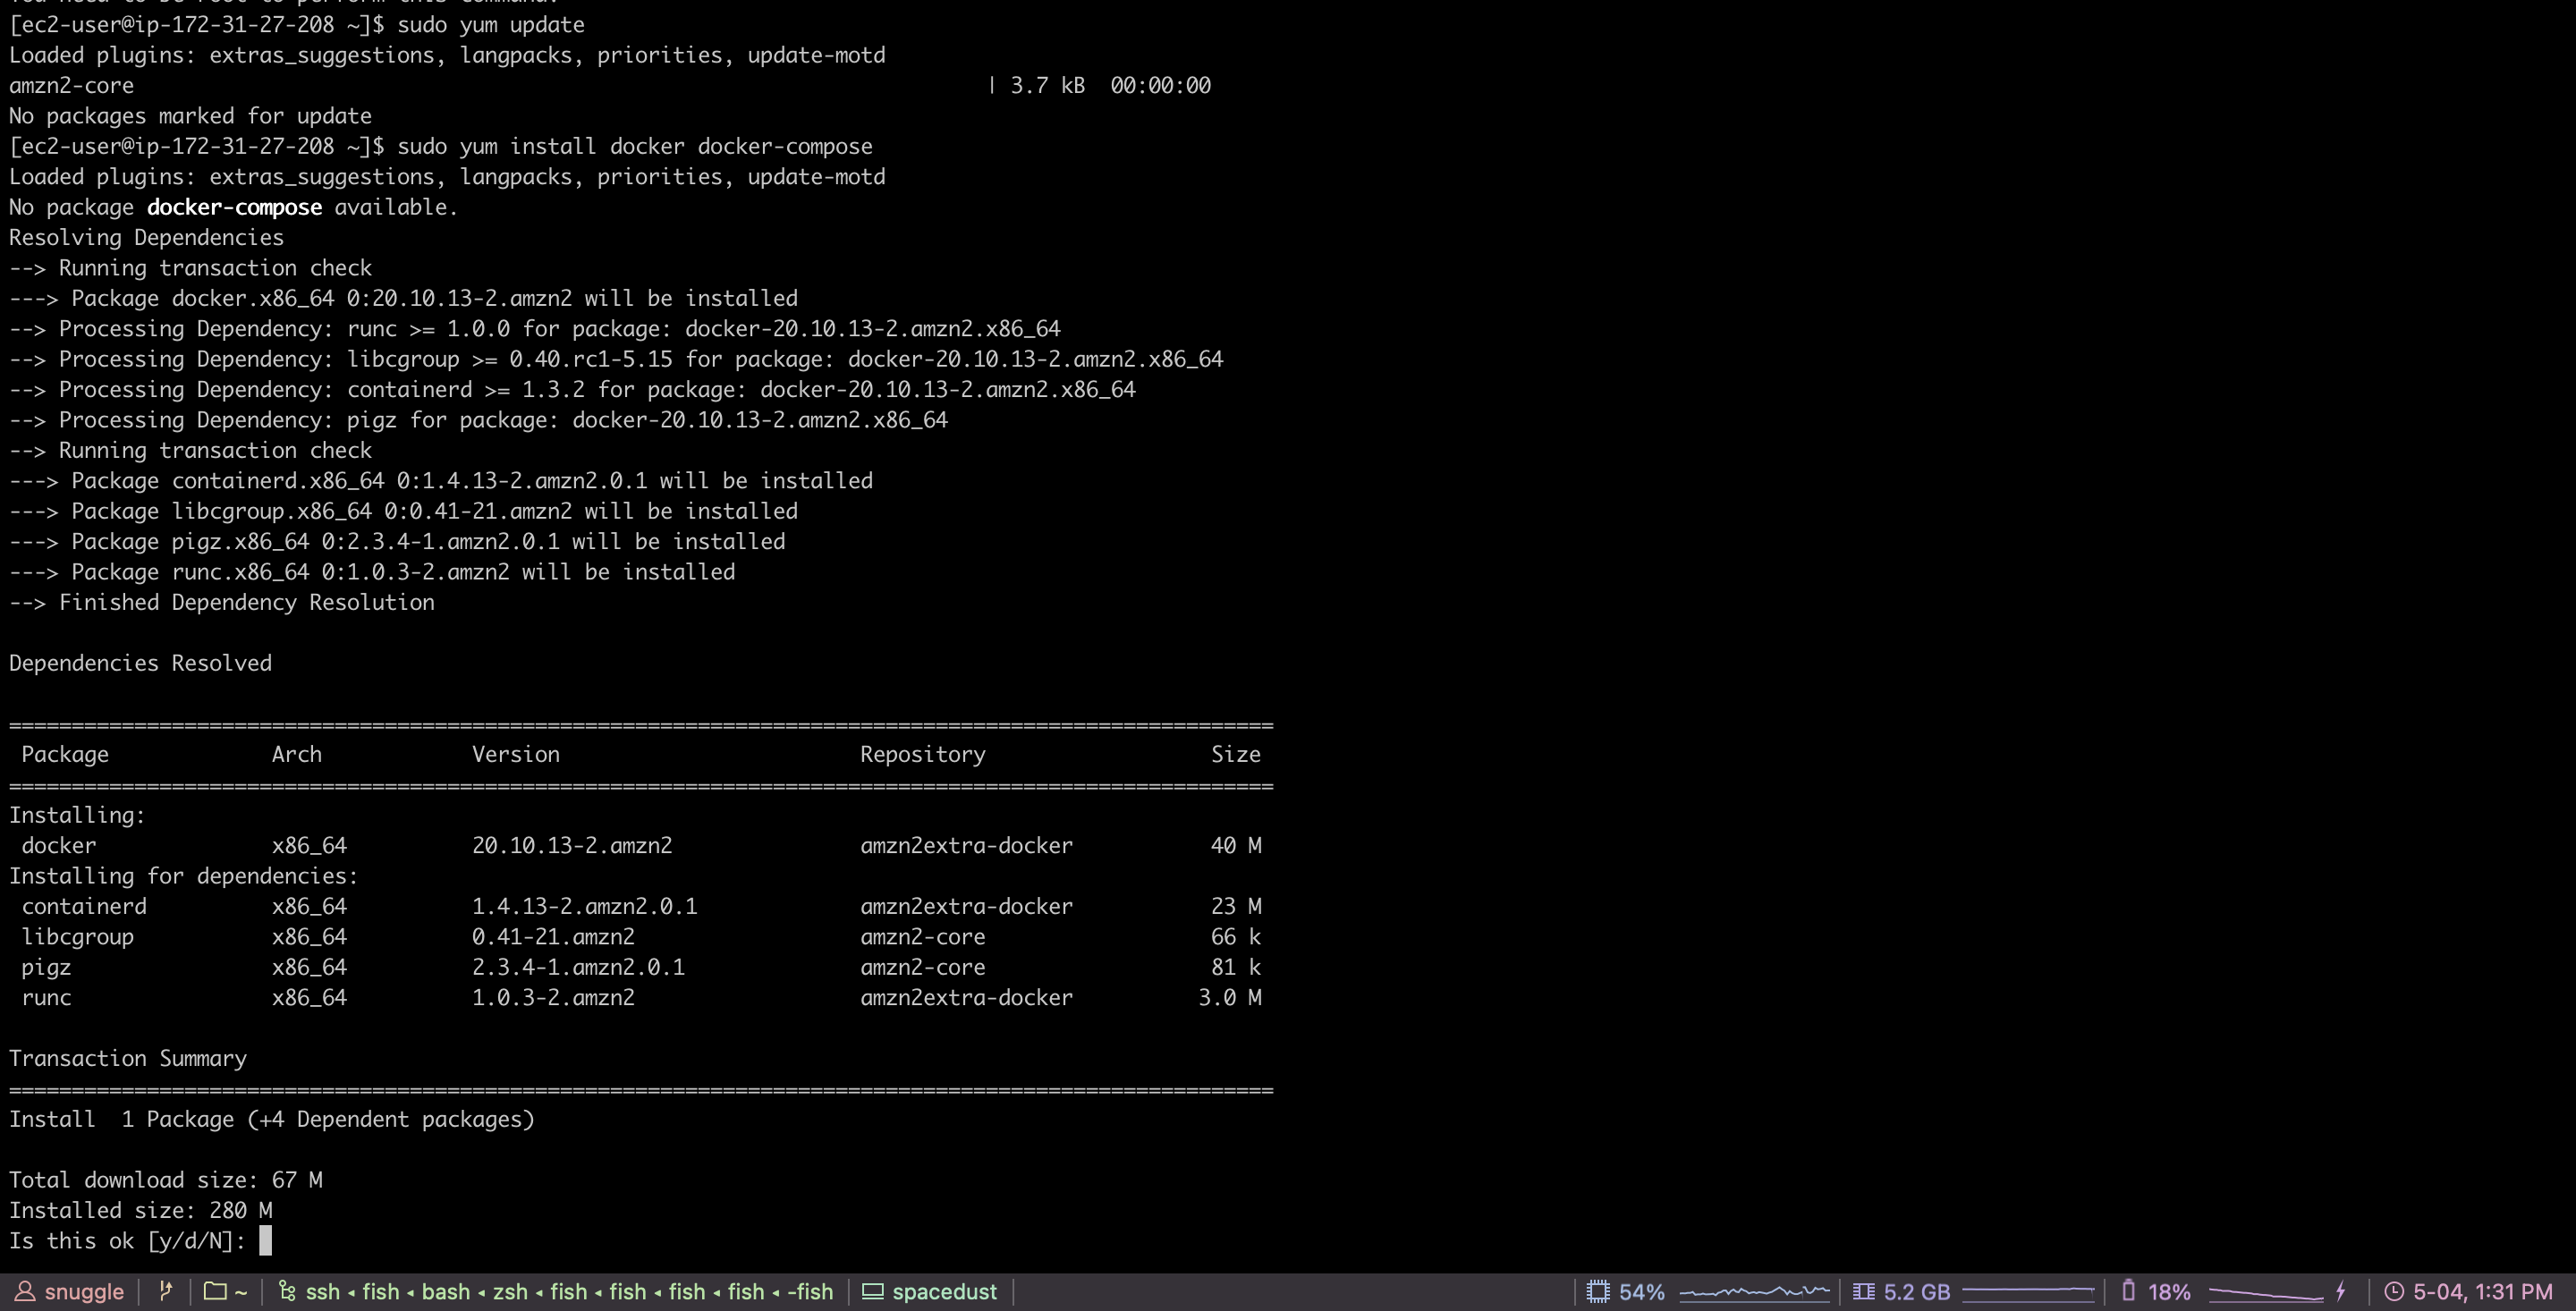
\includegraphics[width=\textwidth]{resources/installing-docker.png}
    \caption{Installing Docker using Package Manager}
    \label{fig:installing-docker}
\end{figure}

\begin{figure}[H]
    \centering
        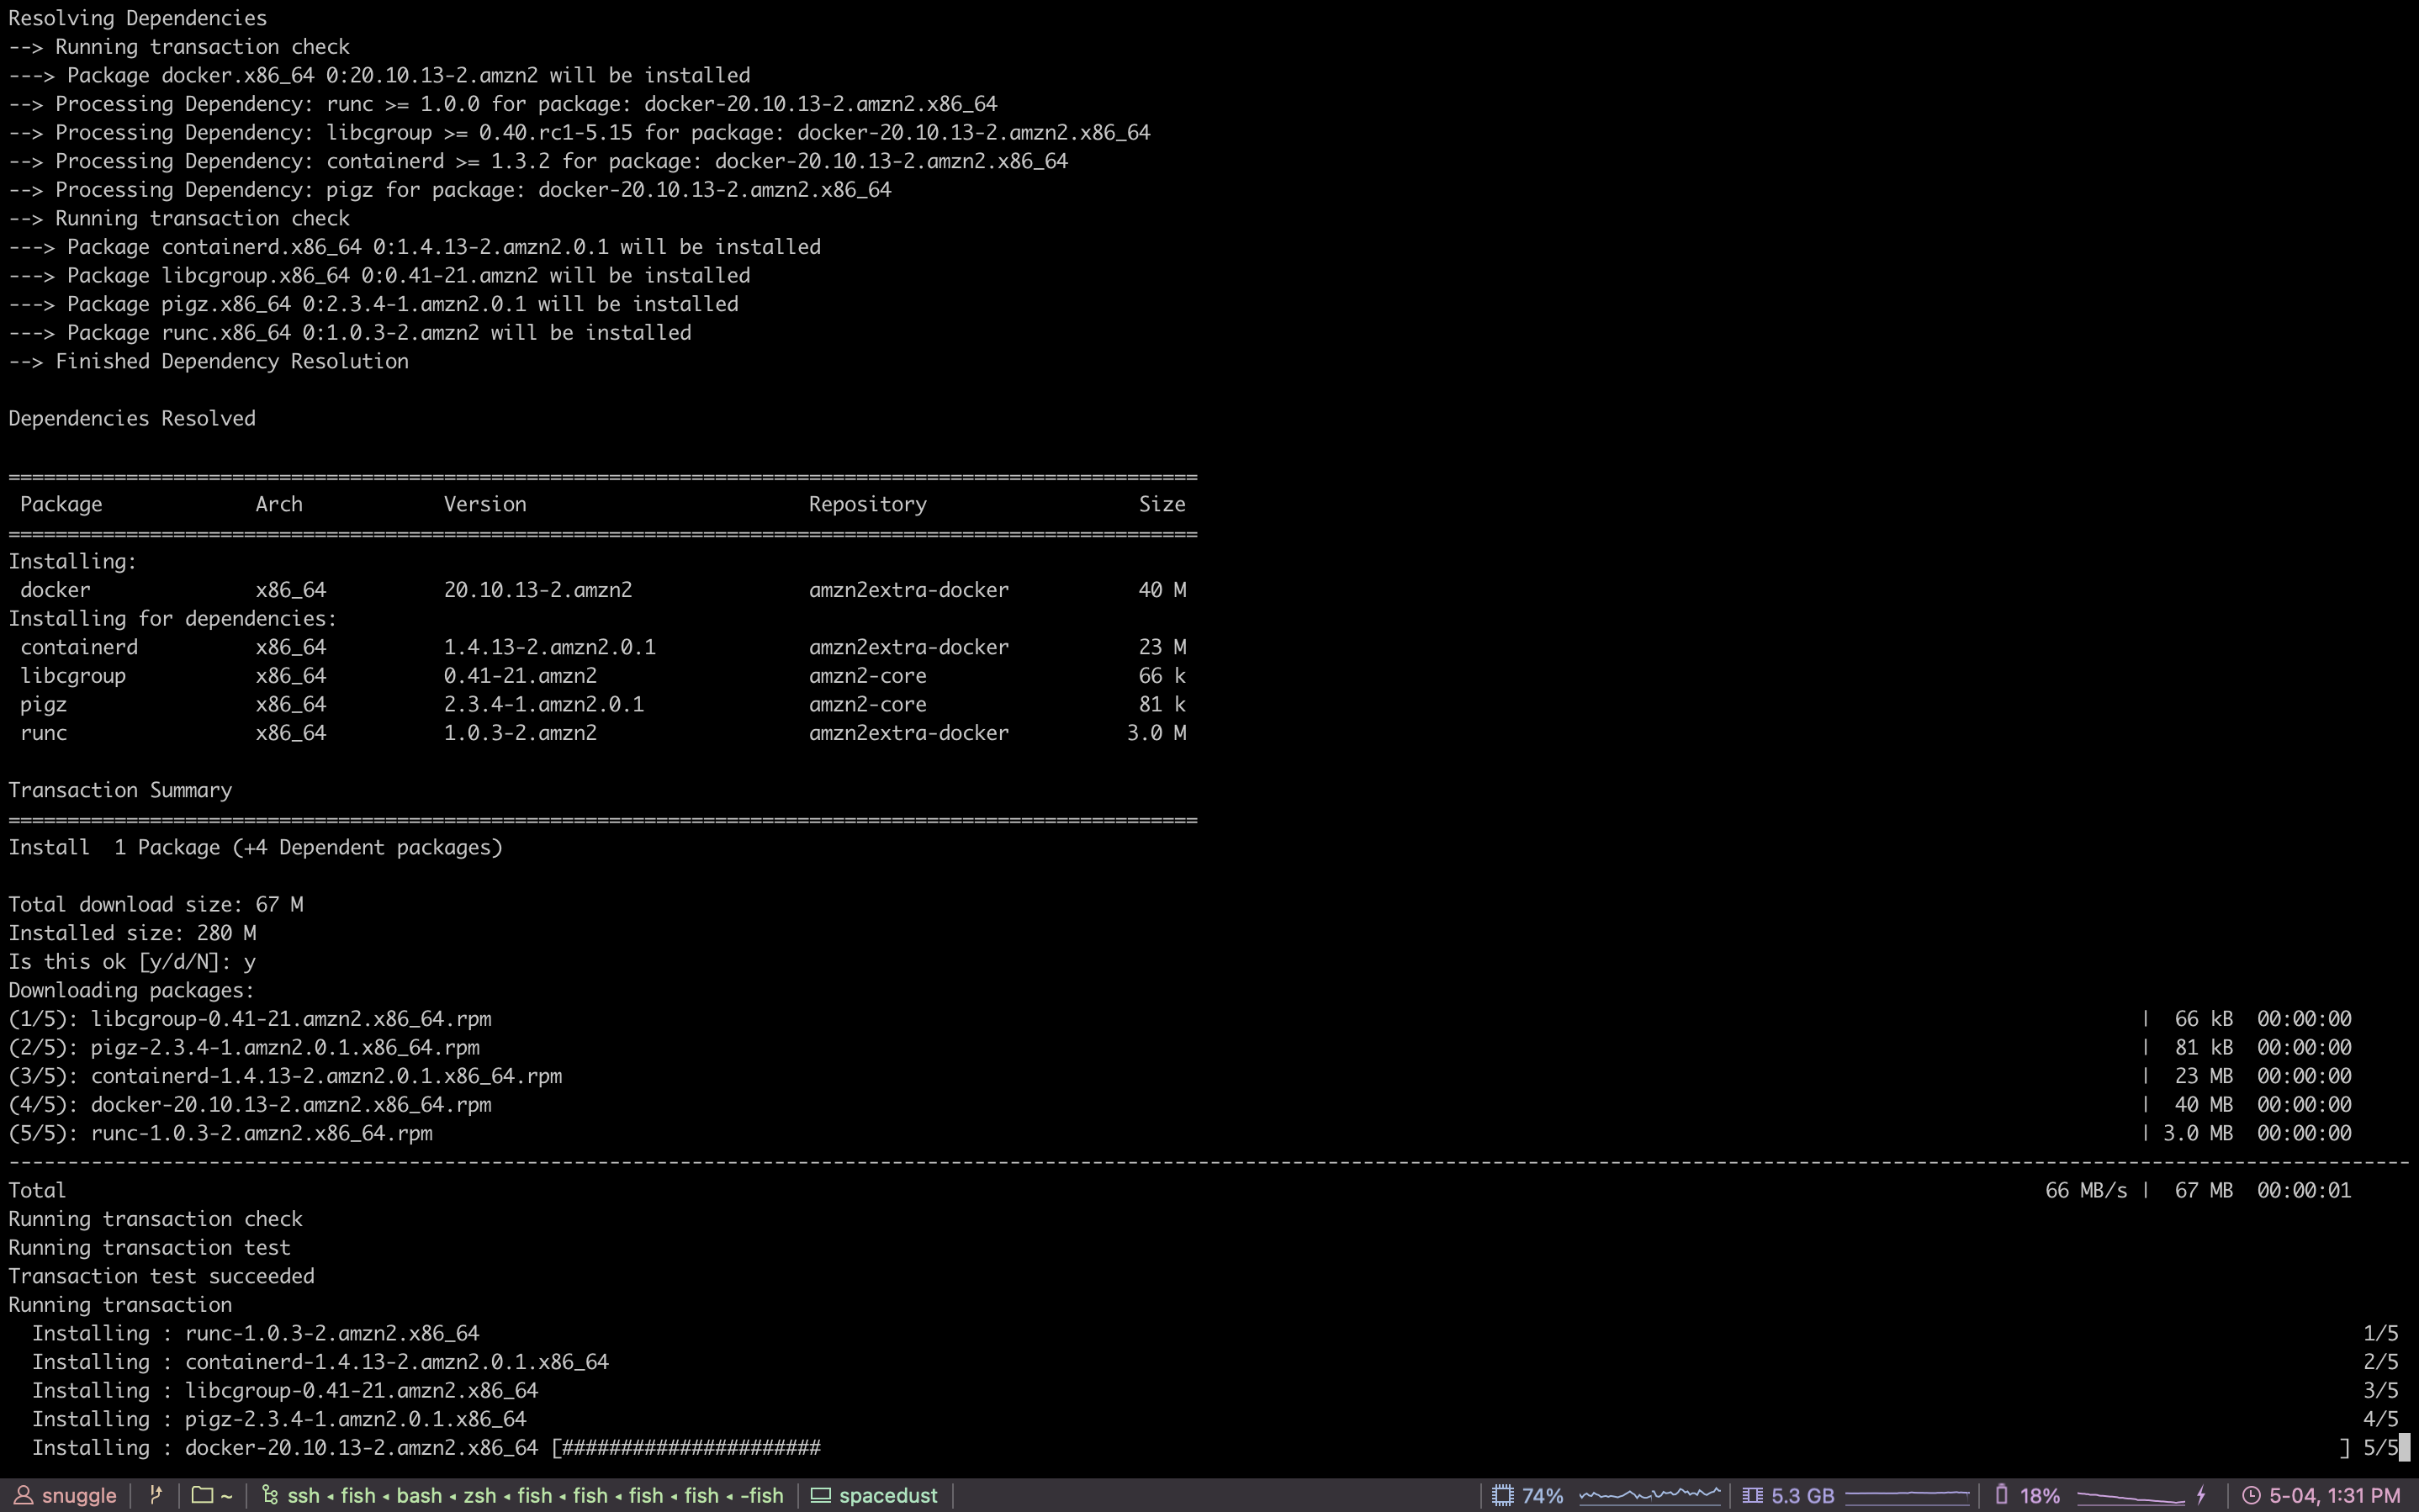
\includegraphics[width=\textwidth]{resources/installing-docker-2.png}
    \caption{Installing Docker using Package Manager (In Progress)}
    \label{fig:installing-docker-2}
\end{figure}

\begin{figure}[H]
    \centering
        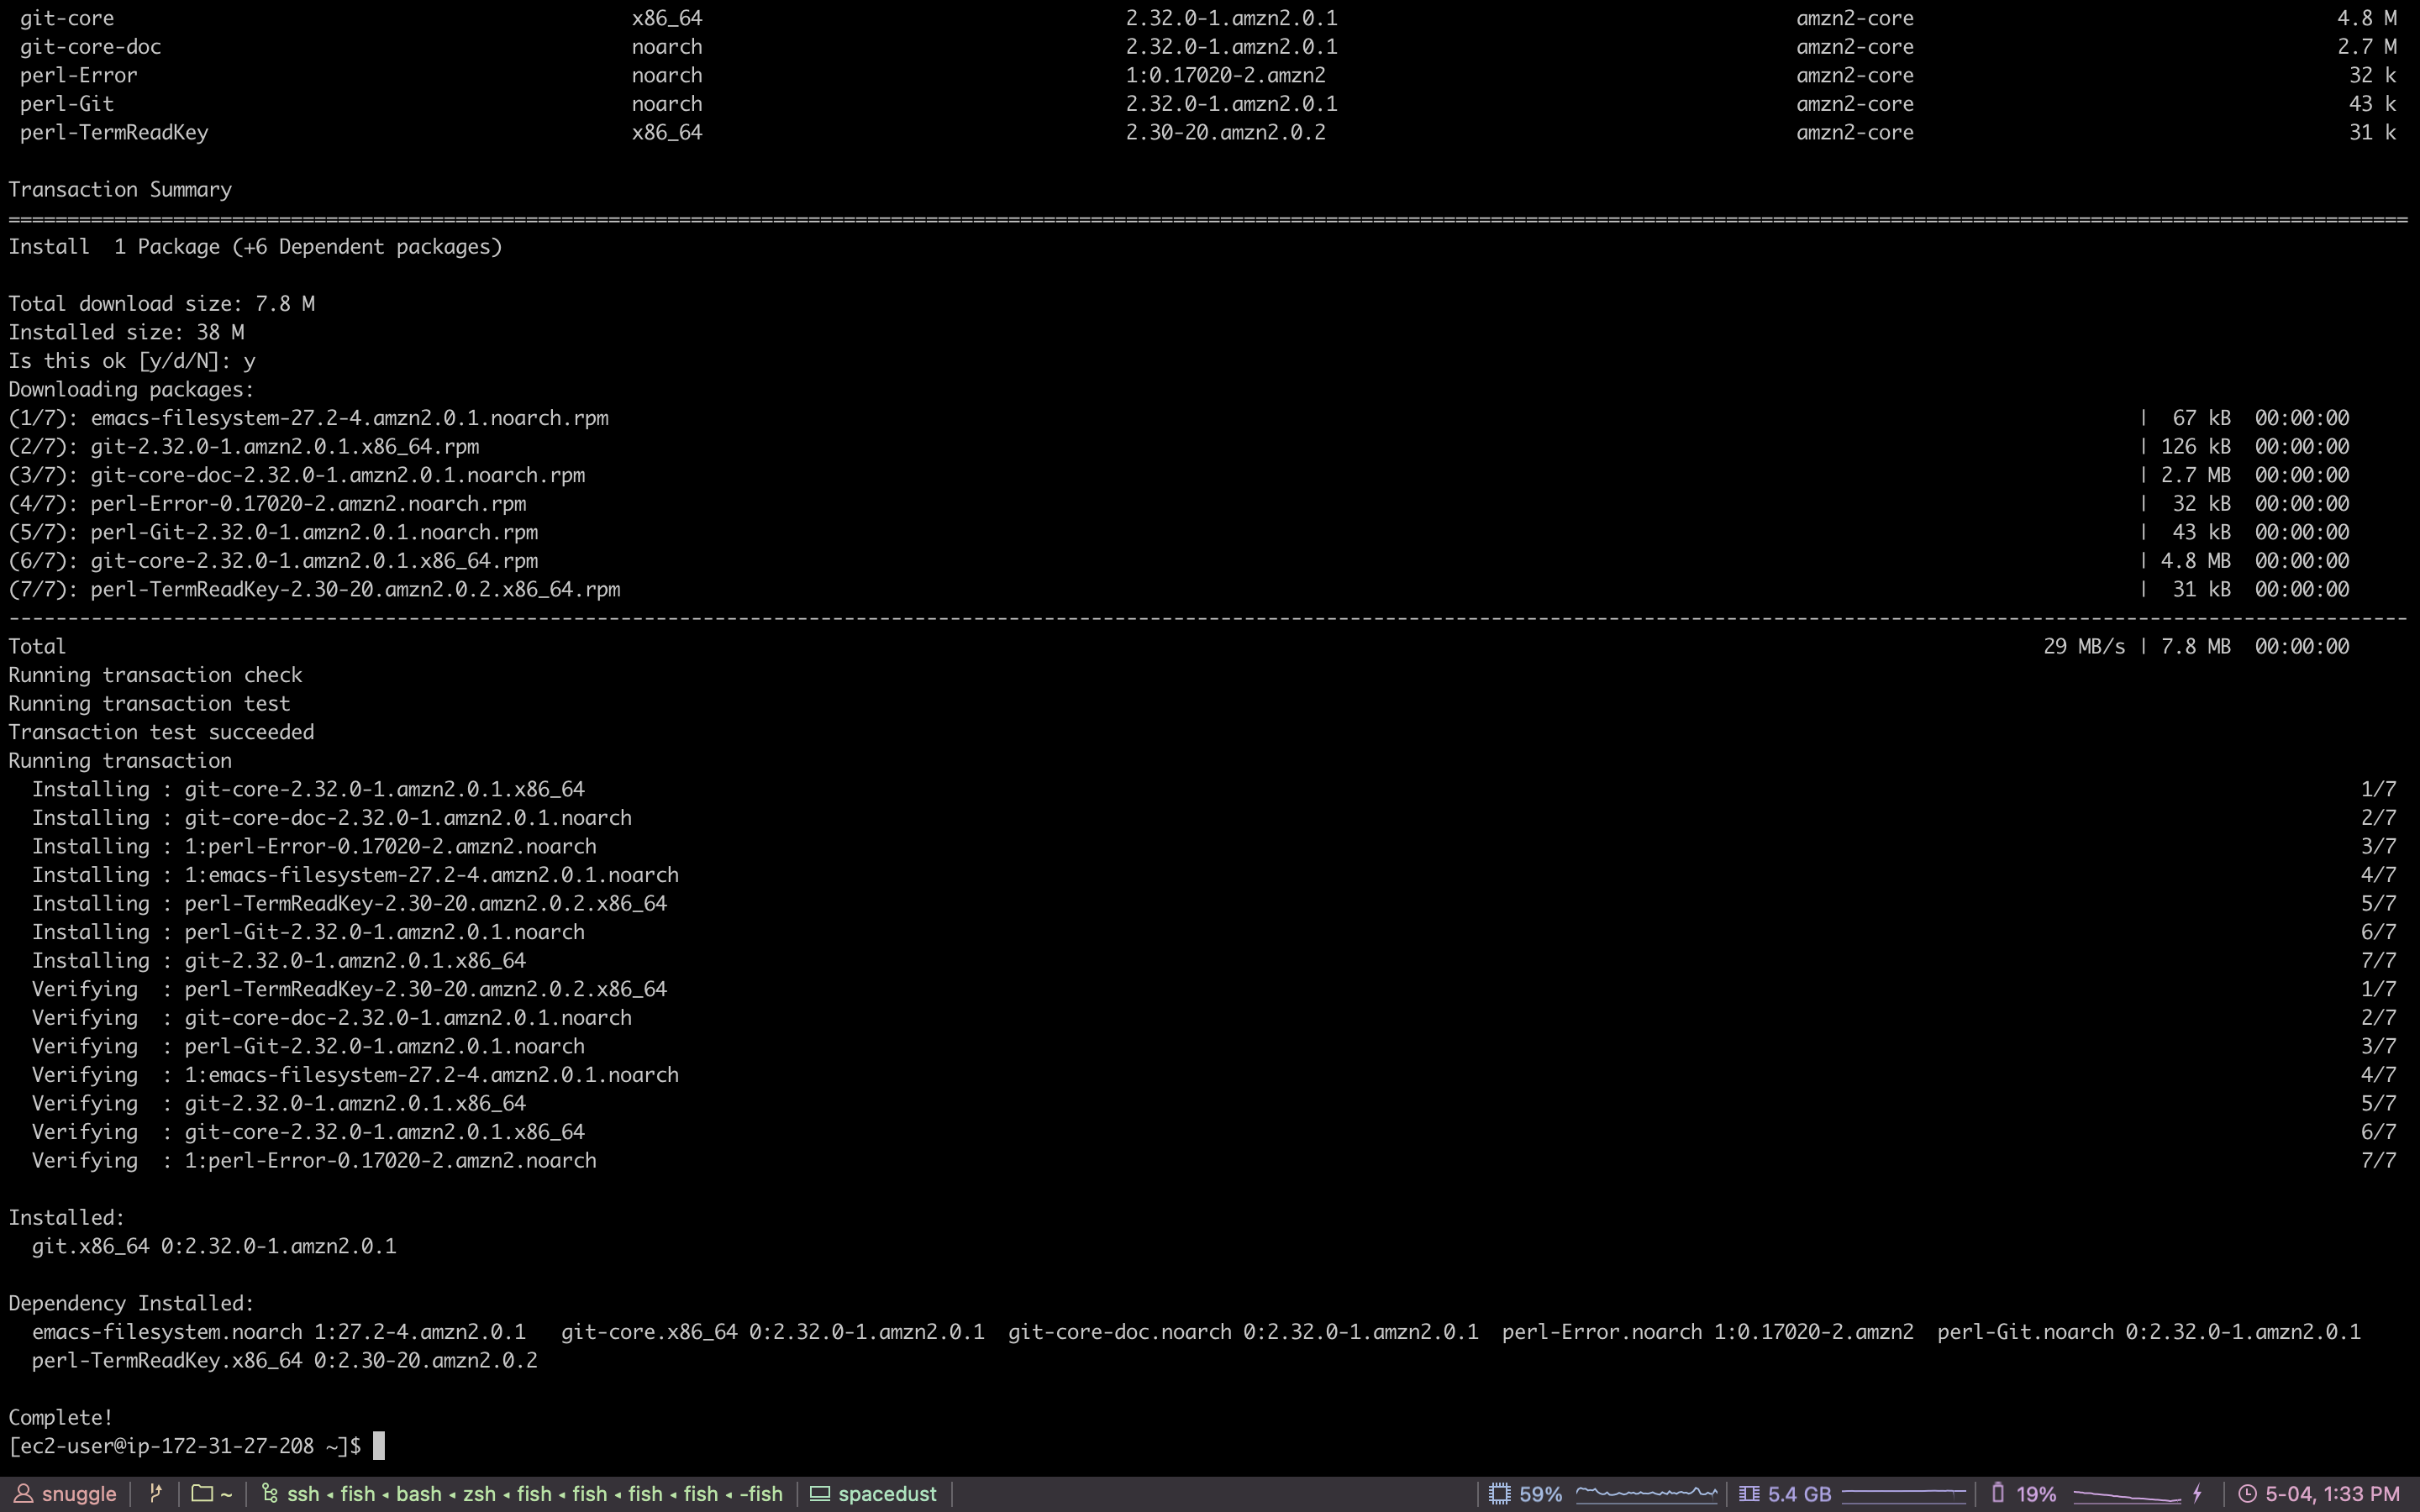
\includegraphics[width=\textwidth]{resources/installing-docker-3.png}
    \caption{Installing Git}
    \label{fig:installing-docker-3}
\end{figure}

\begin{figure}[H]
    \centering
        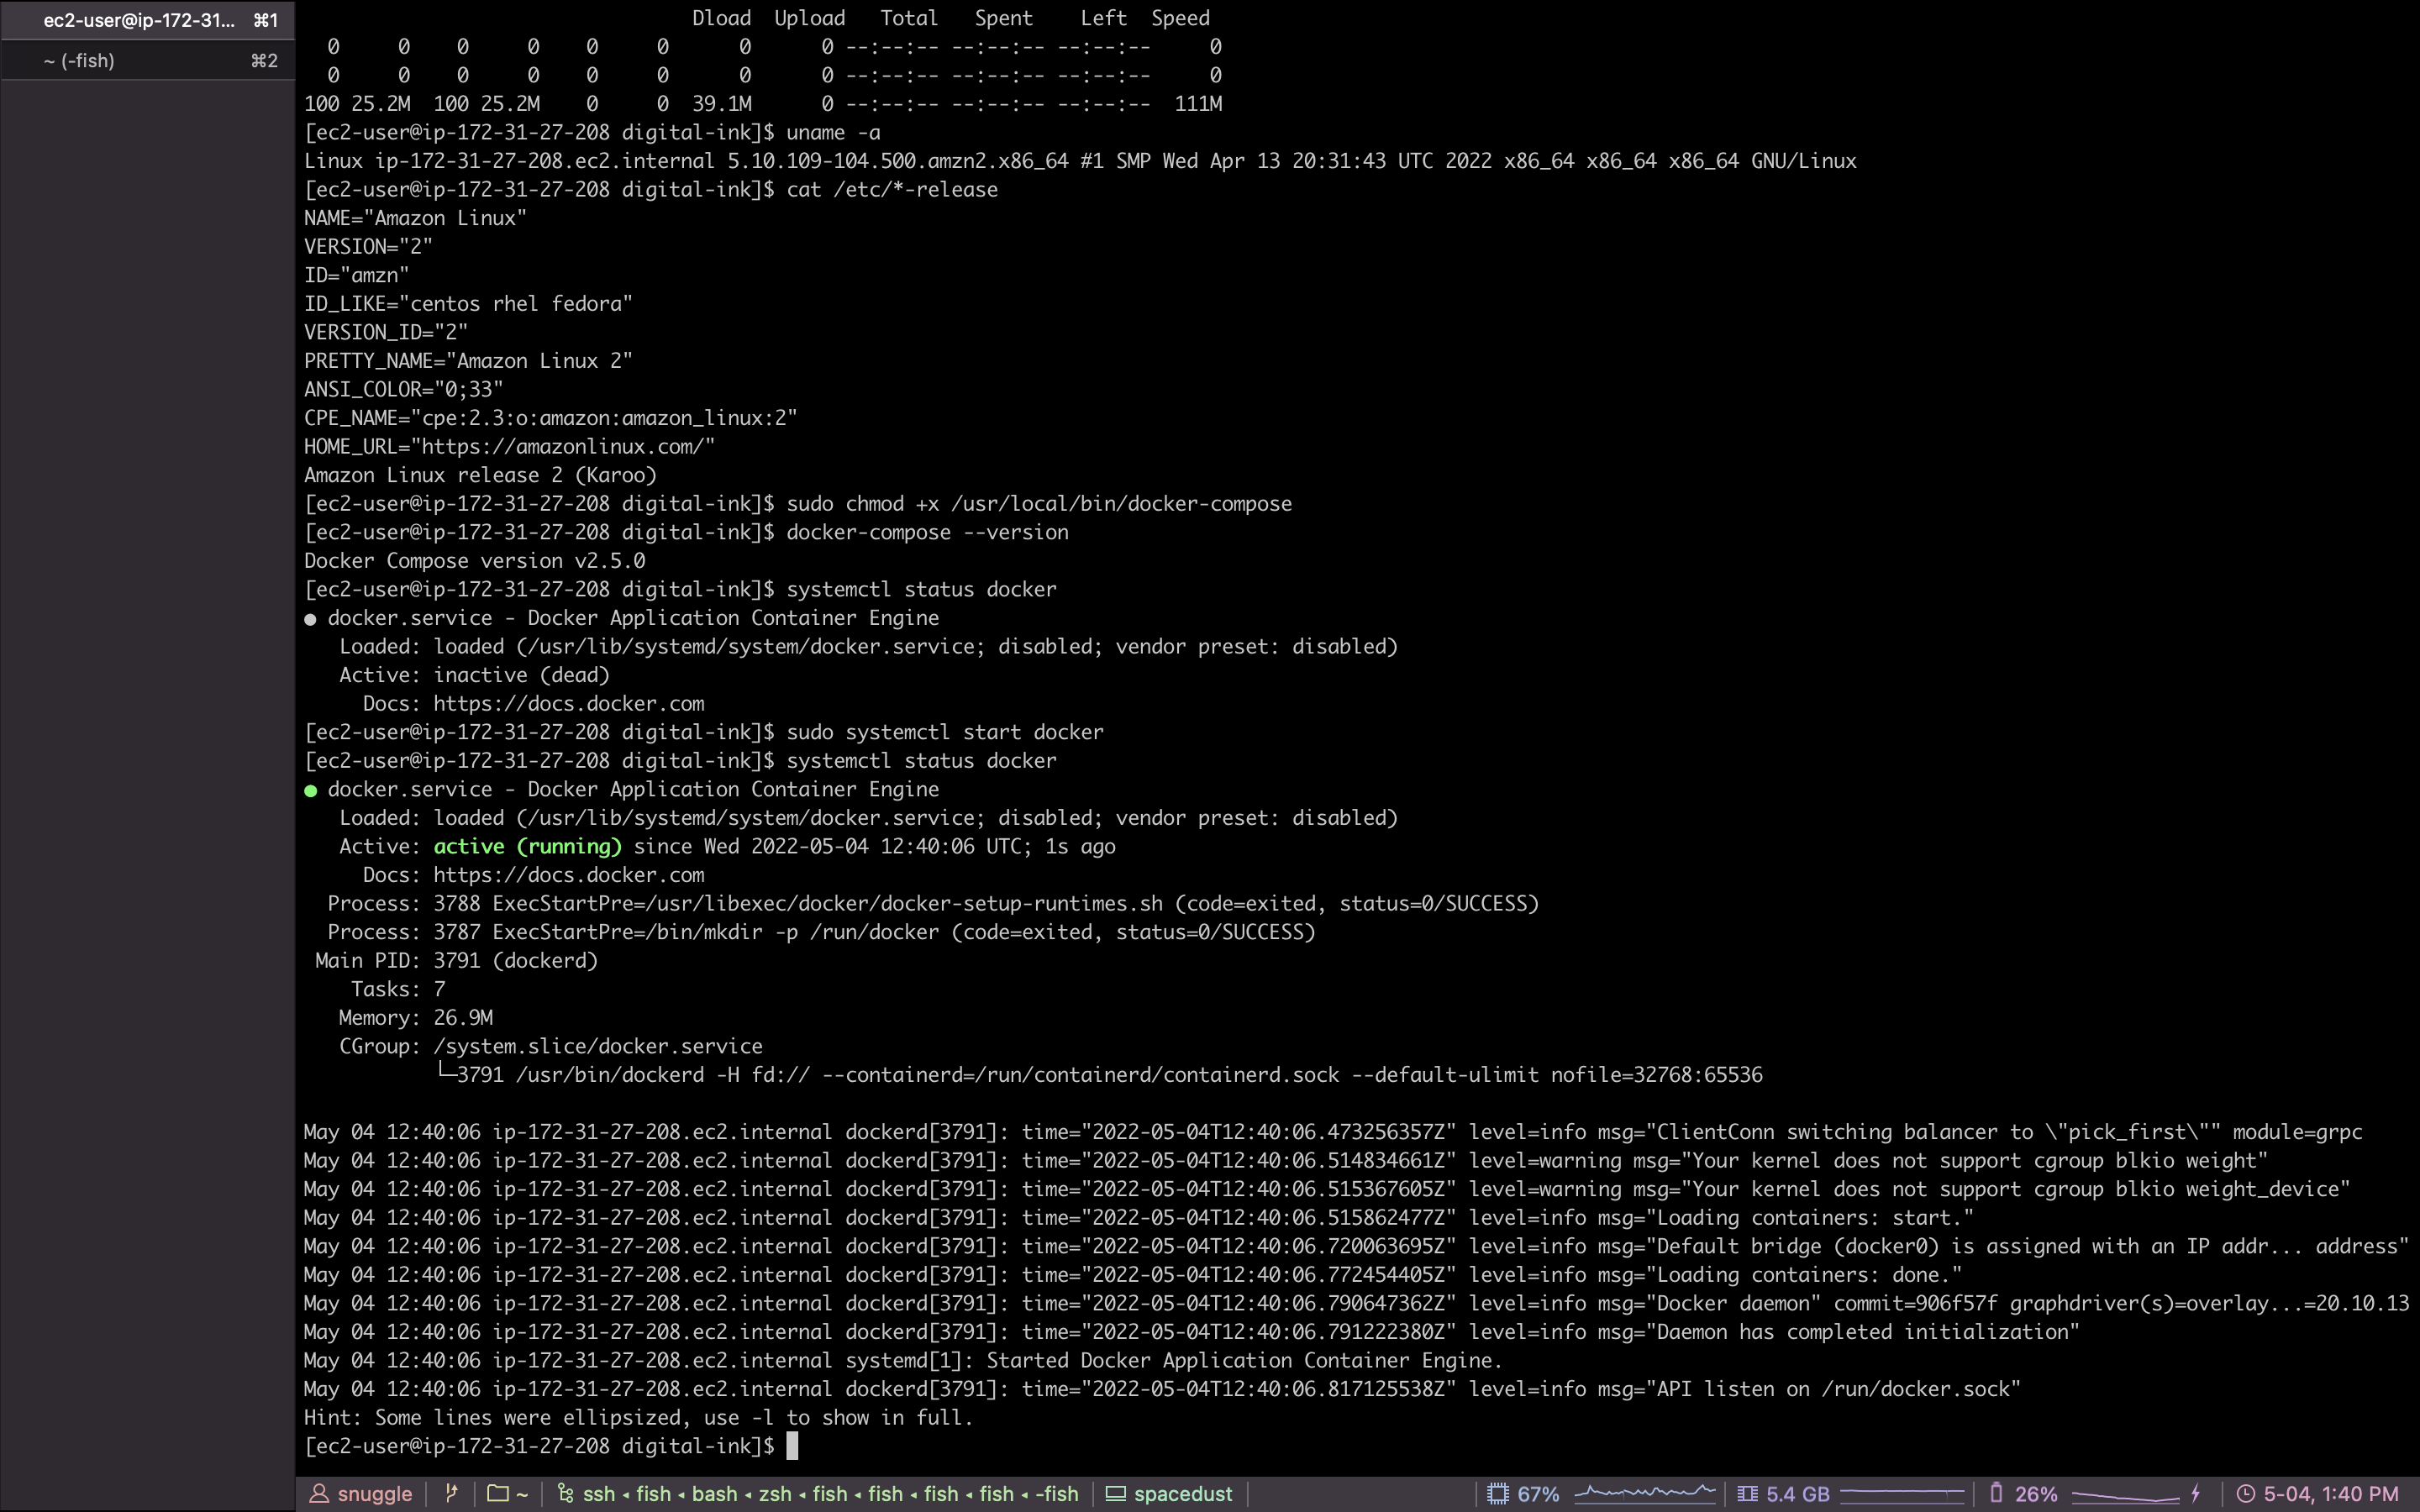
\includegraphics[width=\textwidth]{resources/installing-docker-4.png}
    \caption{Starting Docker systemd Service}
    \label{fig:installing-docker-4}
\end{figure}

\begin{figure}[H]
    \centering
        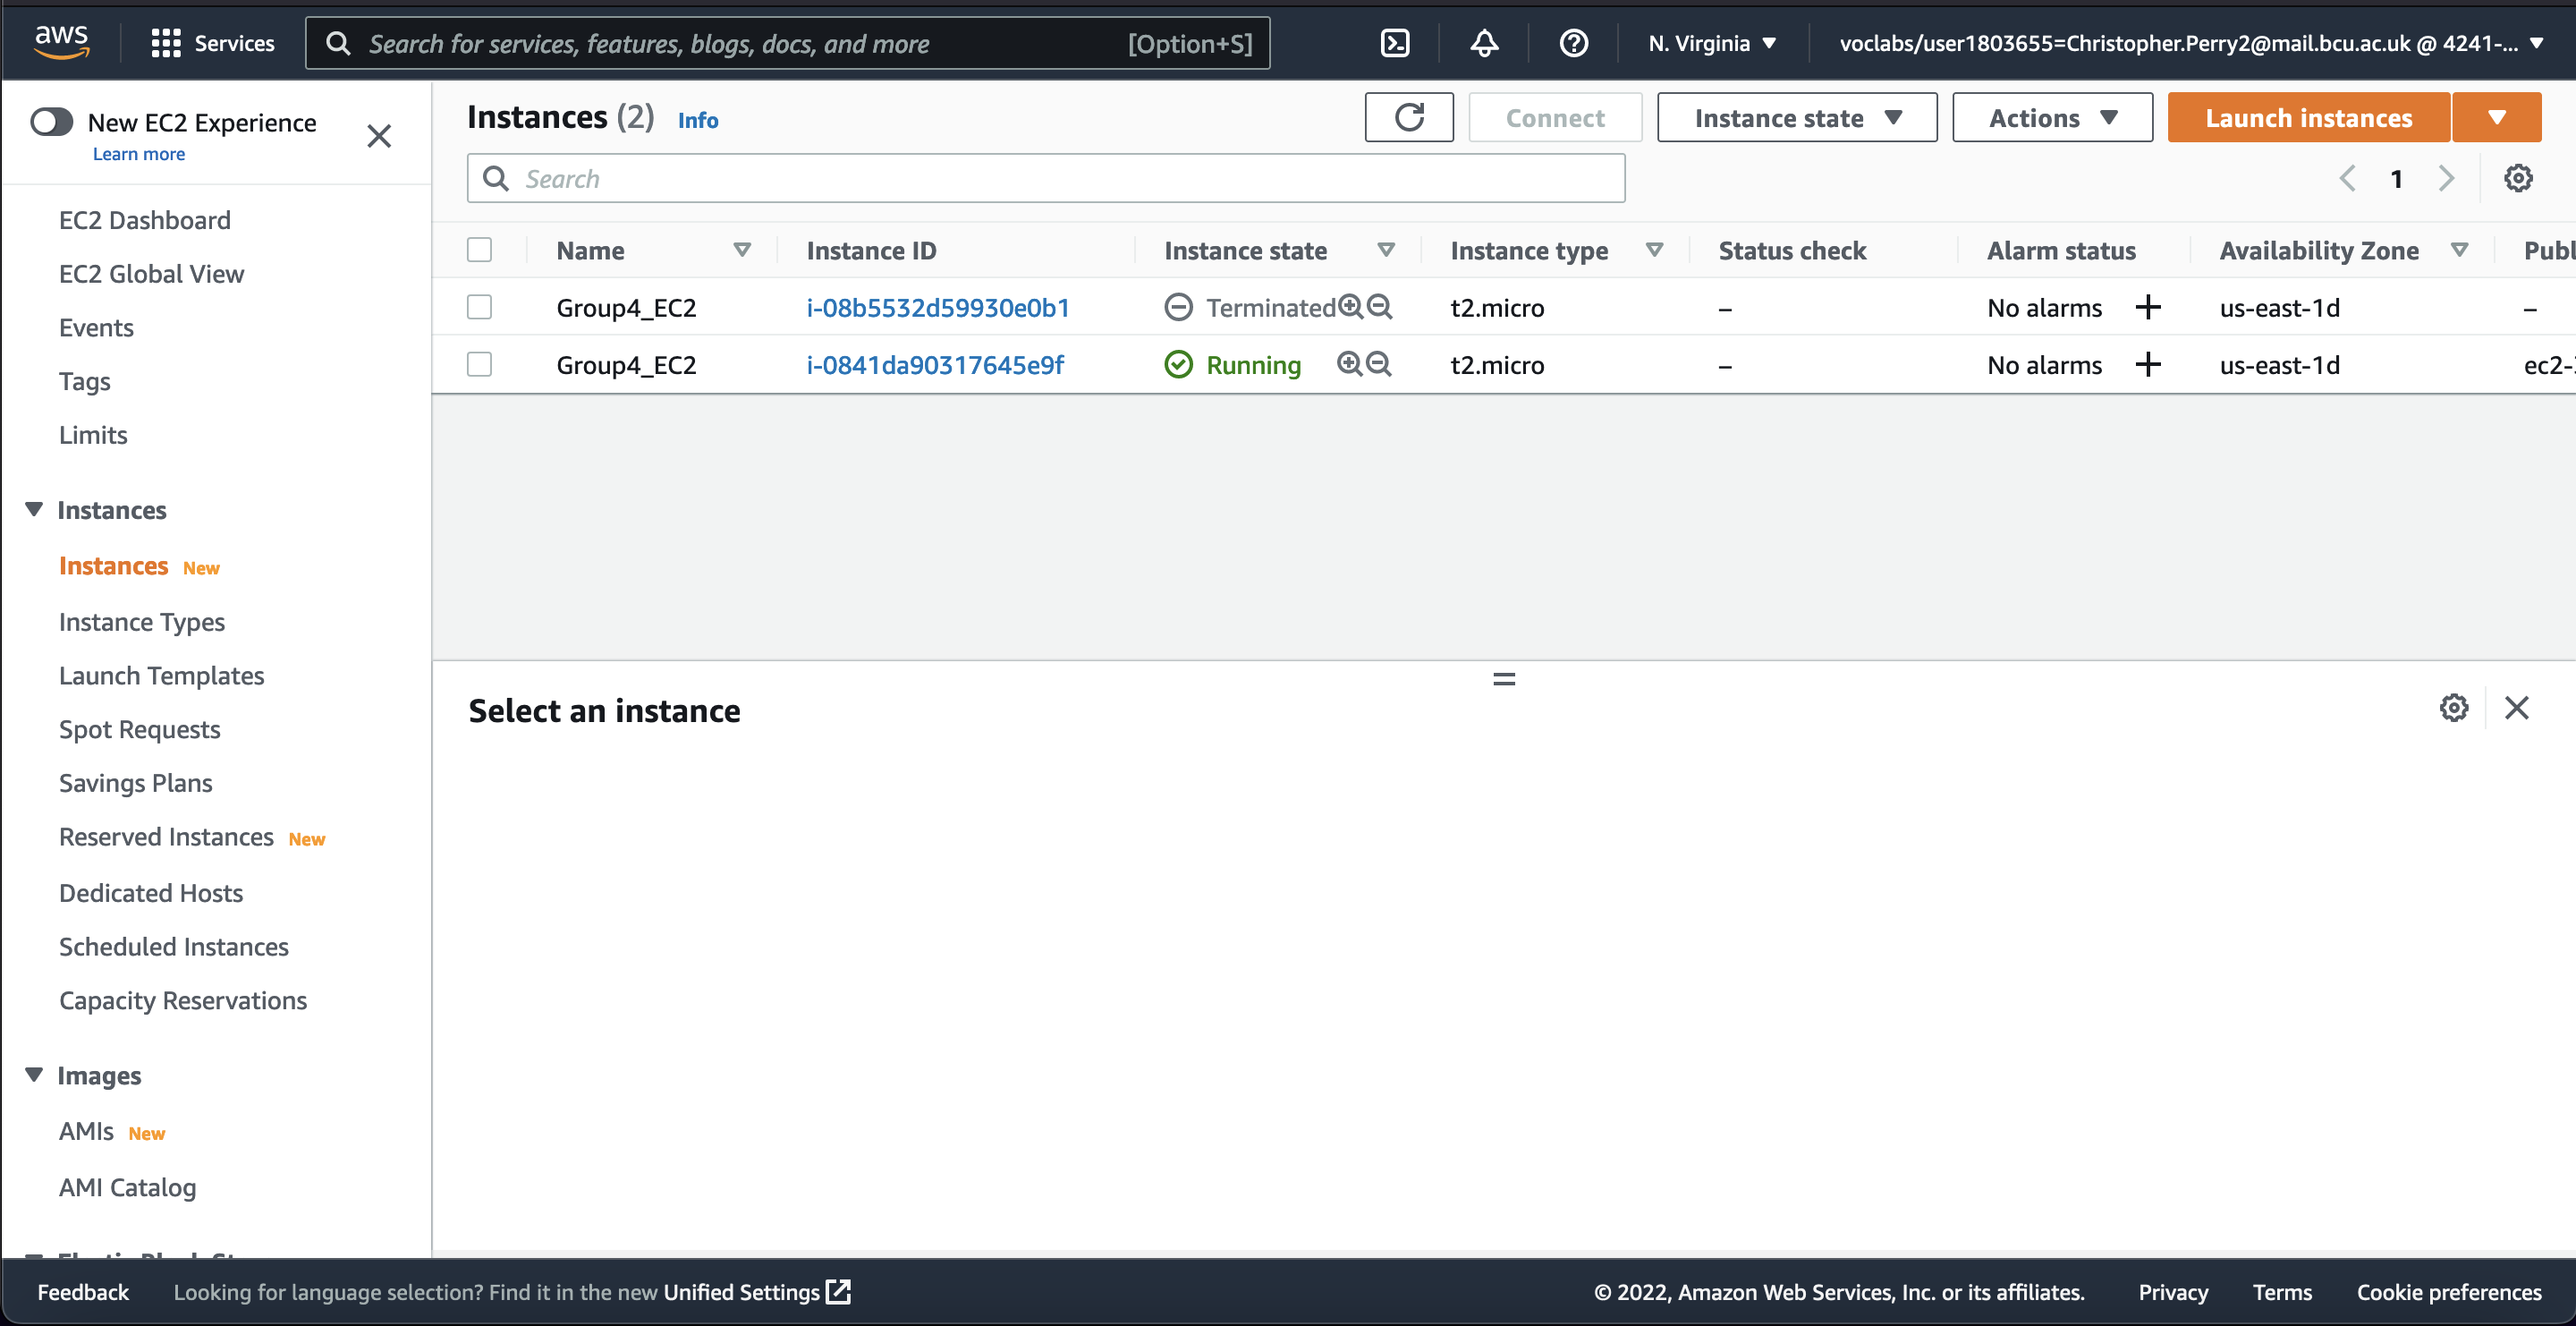
\includegraphics[width=\textwidth]{resources/instances.png}
    \caption{Instances}
    \label{fig:instances}
\end{figure}

\begin{figure}[H]
    \centering
        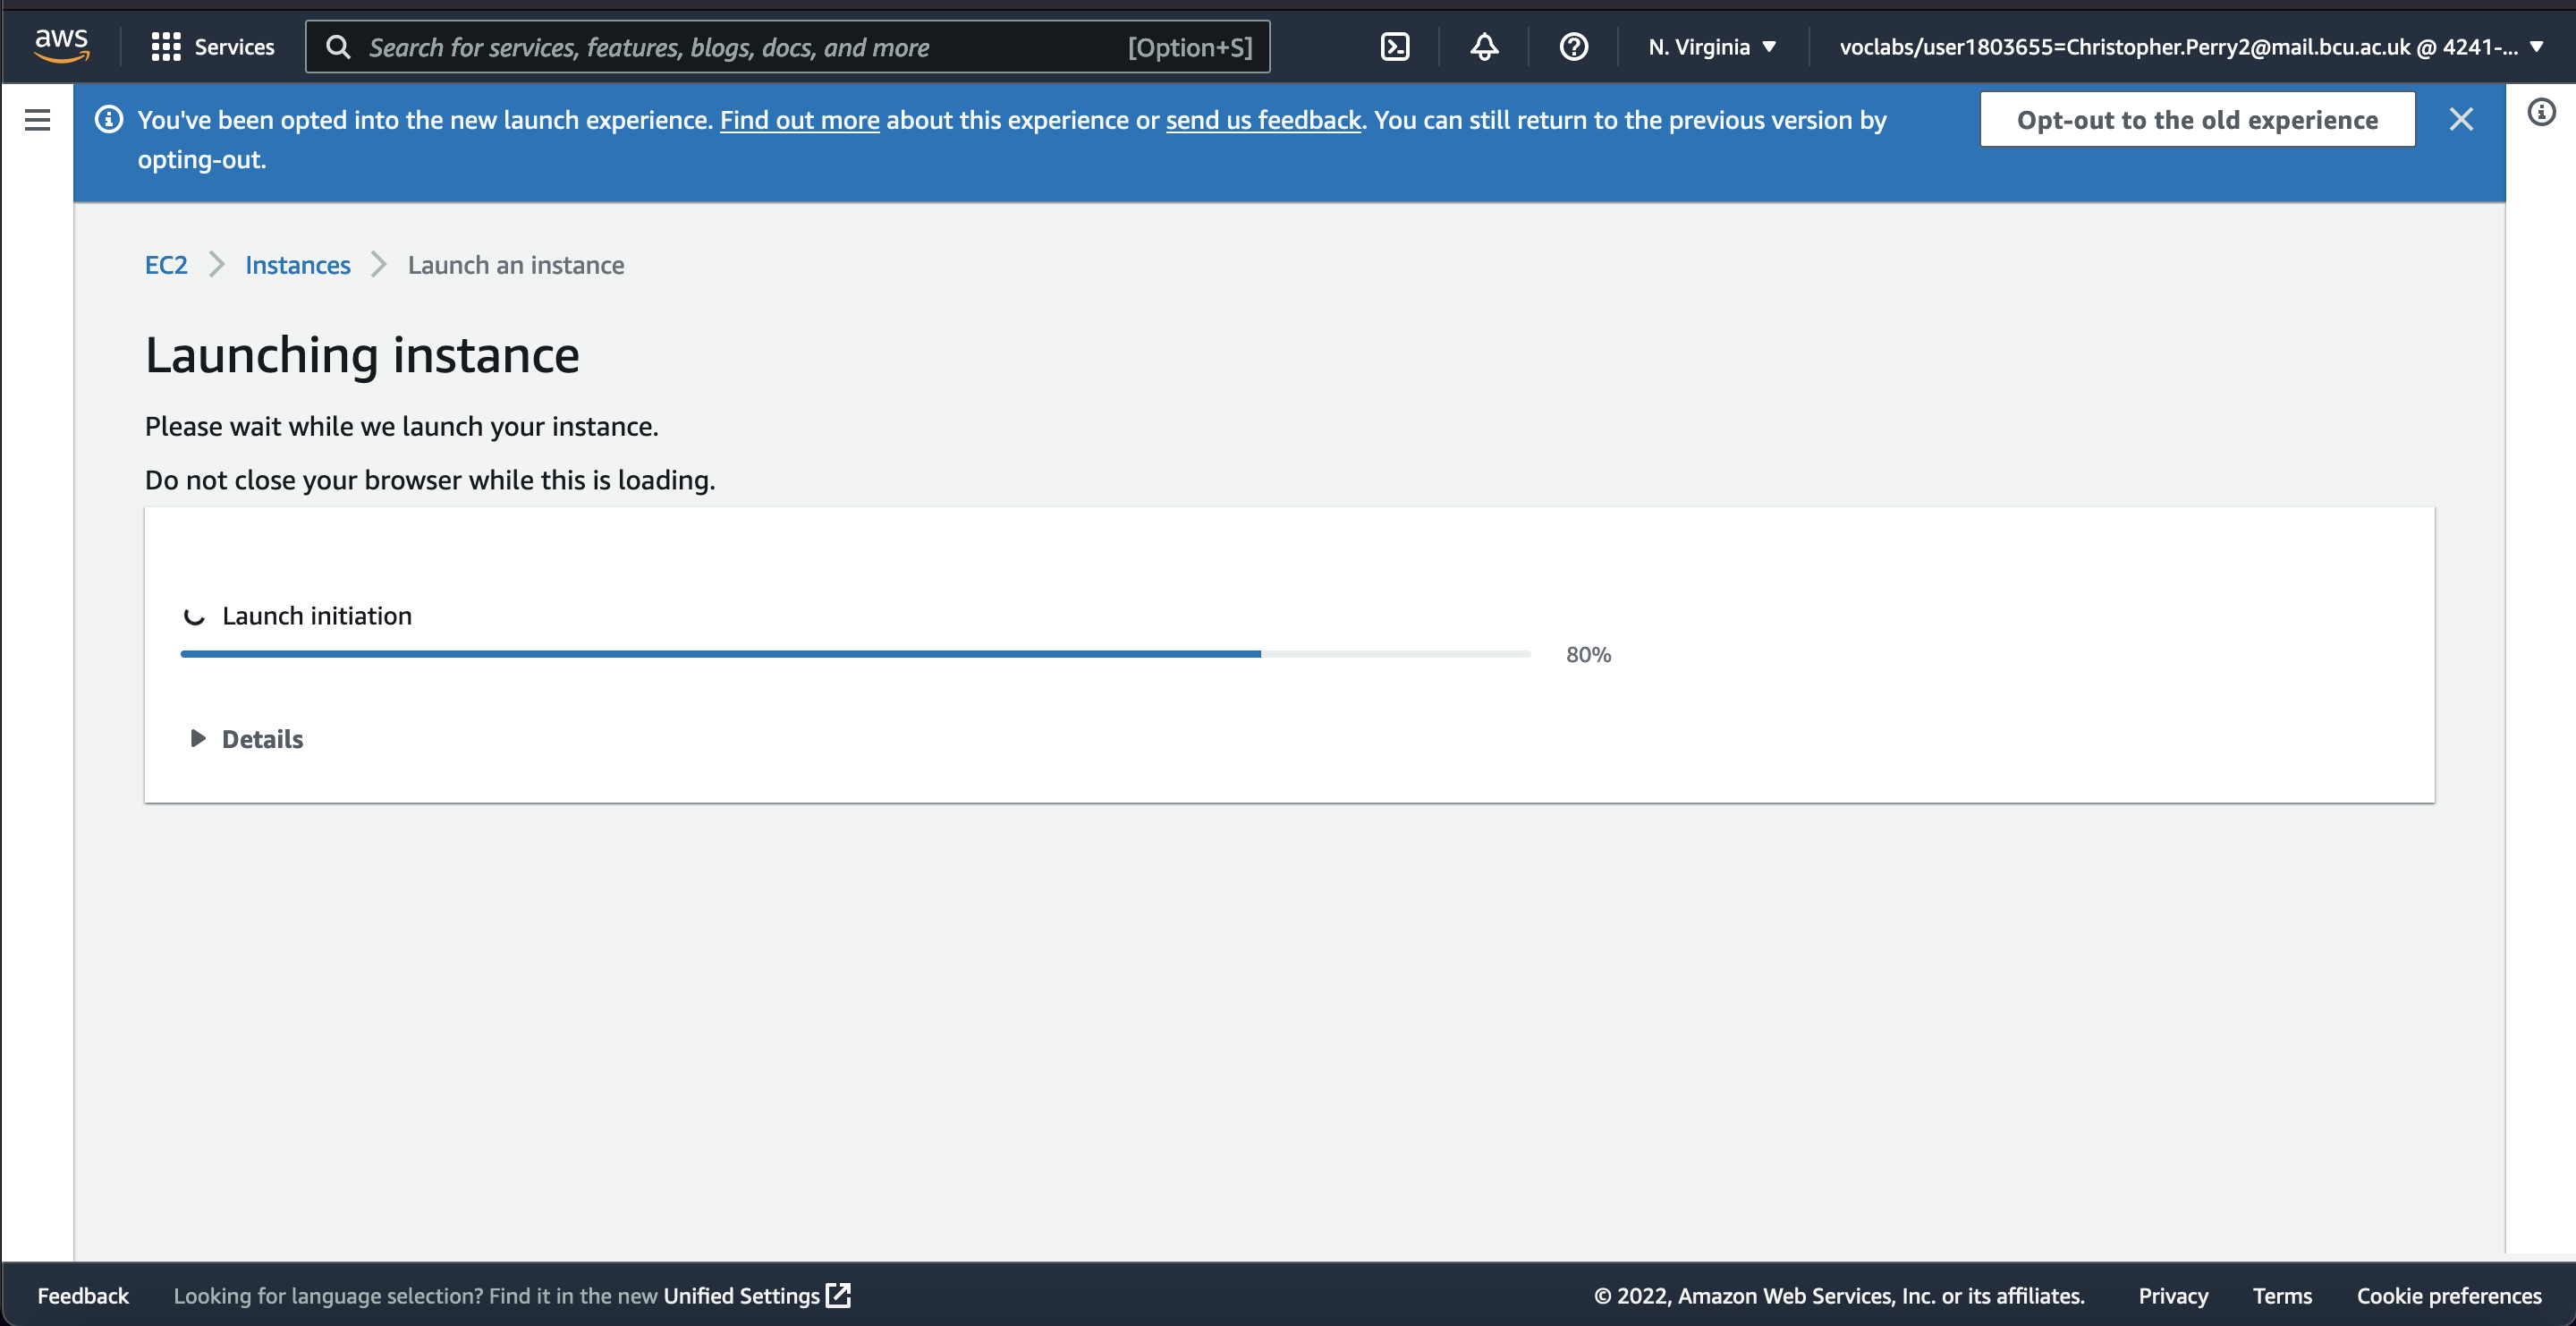
\includegraphics[width=\textwidth]{resources/launching-instance.png}
    \caption{Launching Instance}
    \label{fig:launching-instance}
\end{figure}

\begin{figure}[H]
    \centering
        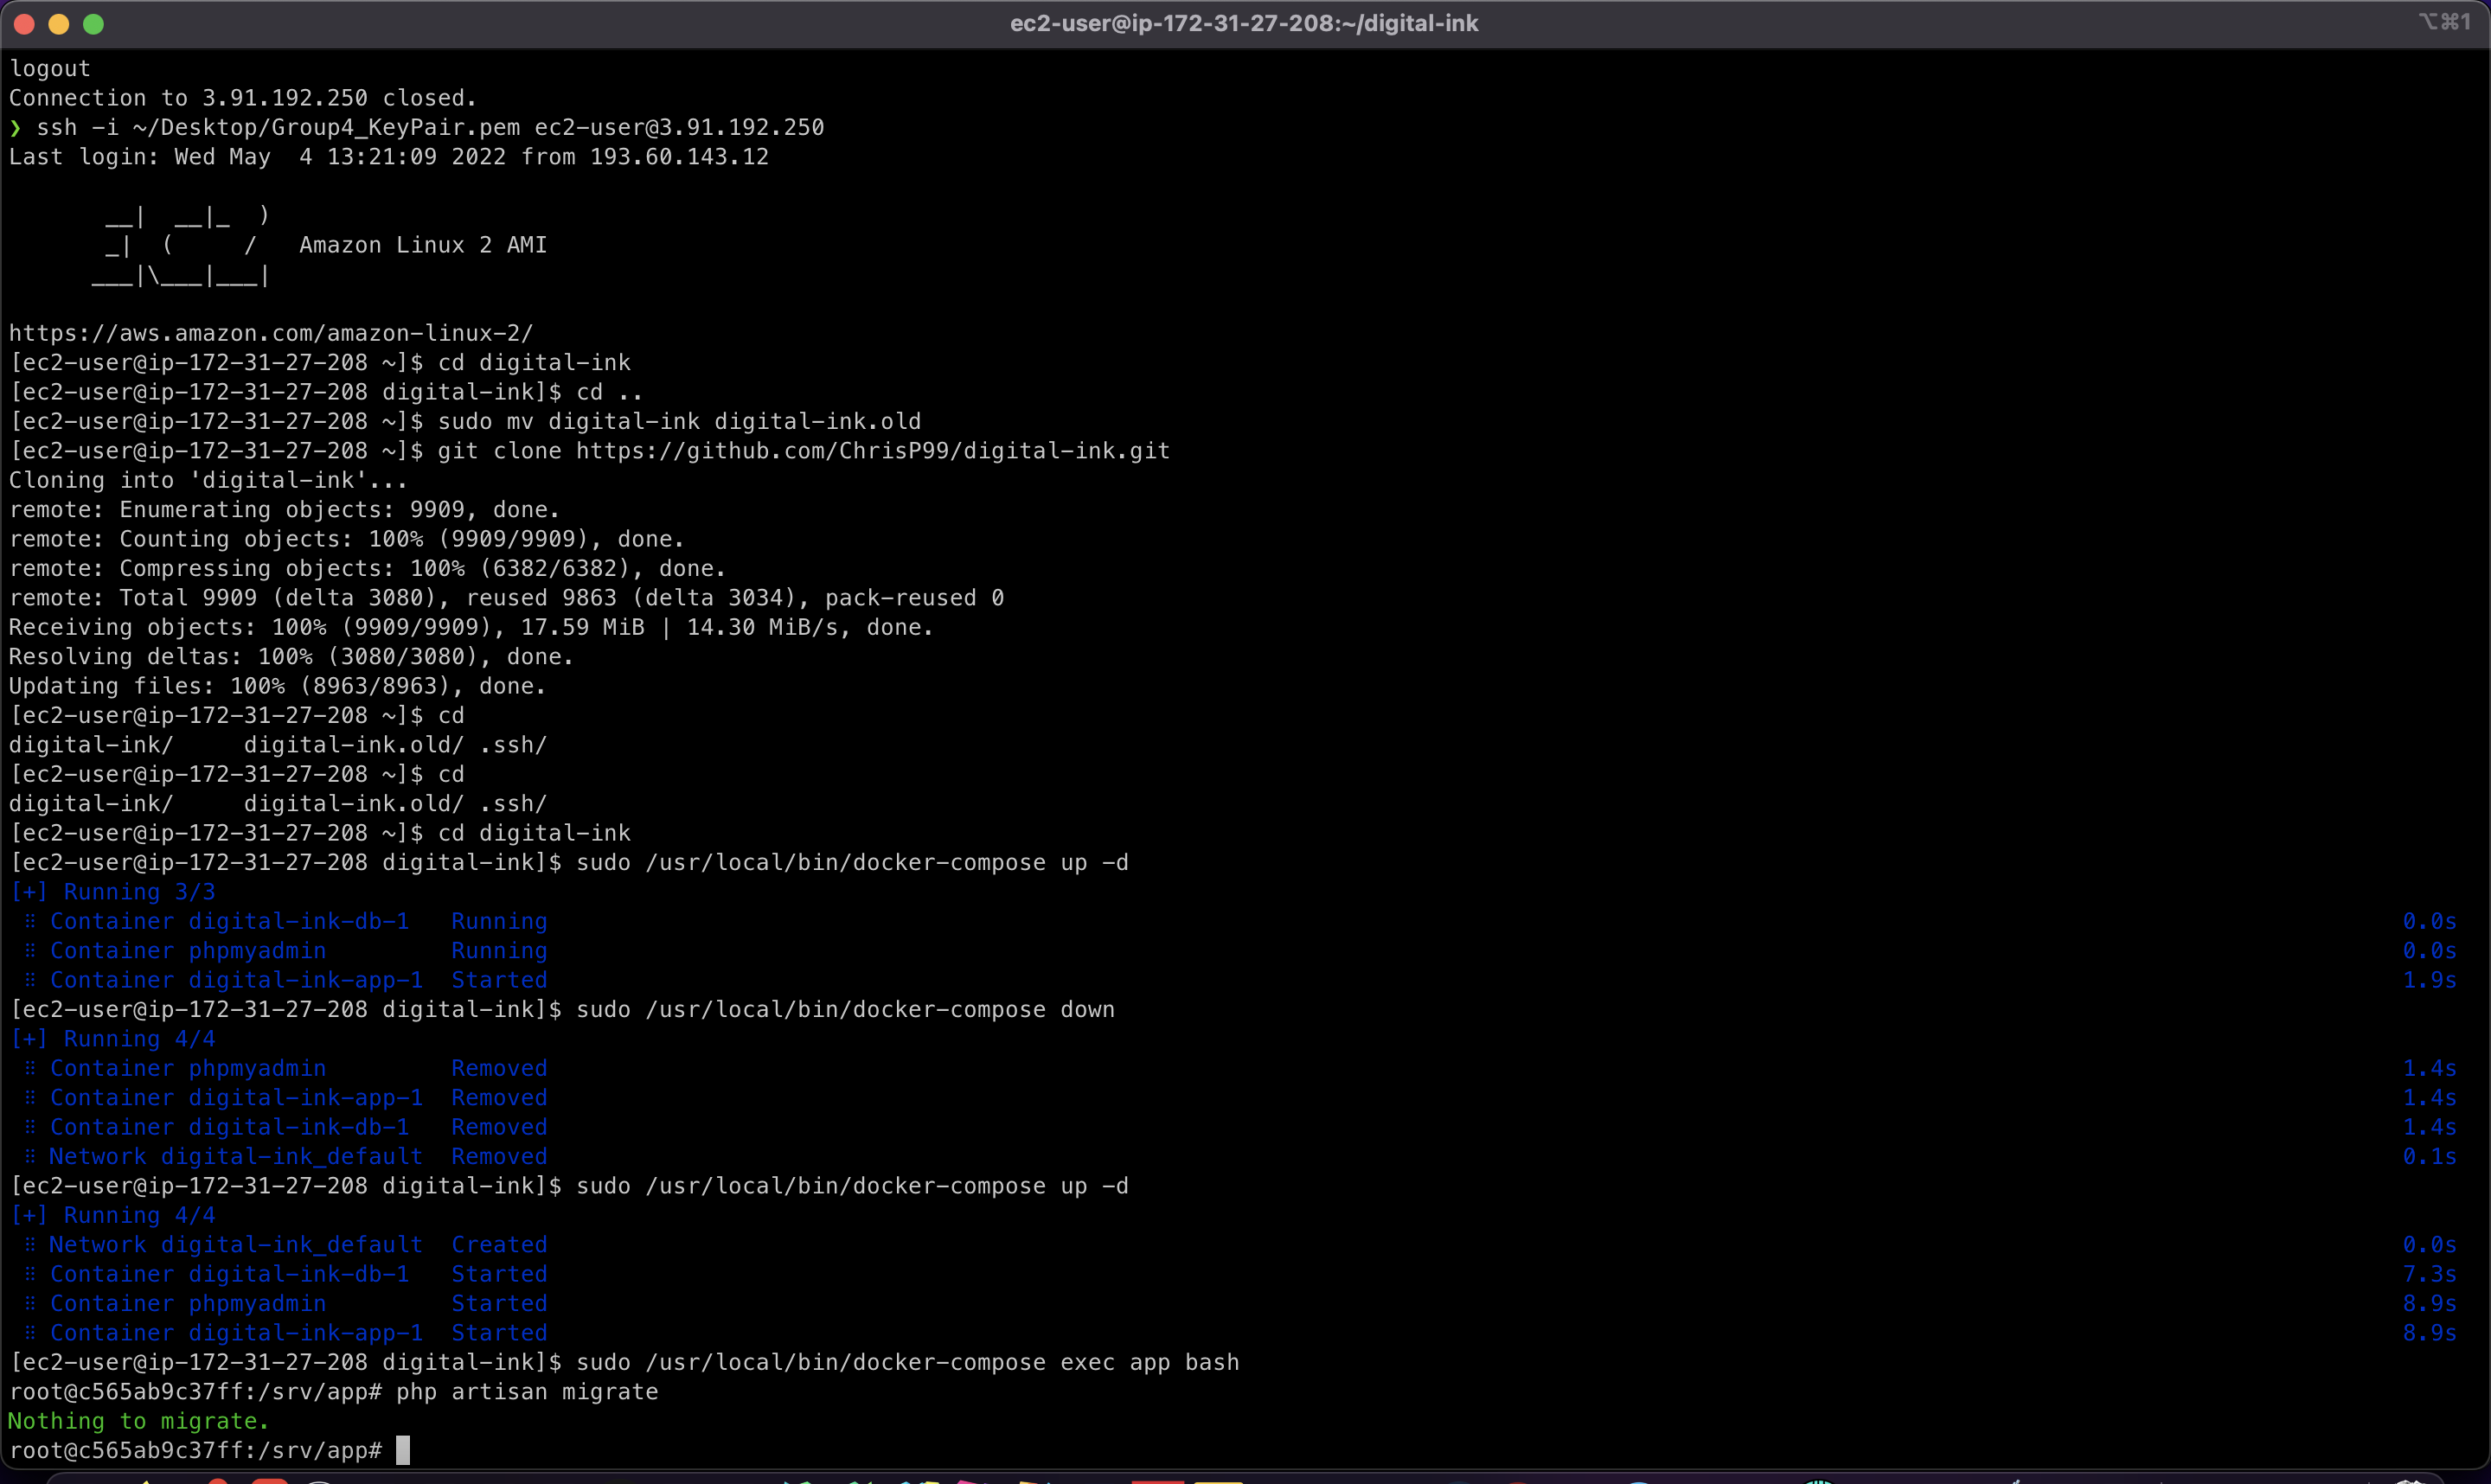
\includegraphics[width=\textwidth]{resources/log-in-with-key-pair.png}
    \caption{Log In with Key Pair}
    \label{fig:log-in-with-key-pair}
\end{figure}

\begin{figure}[H]
    \centering
        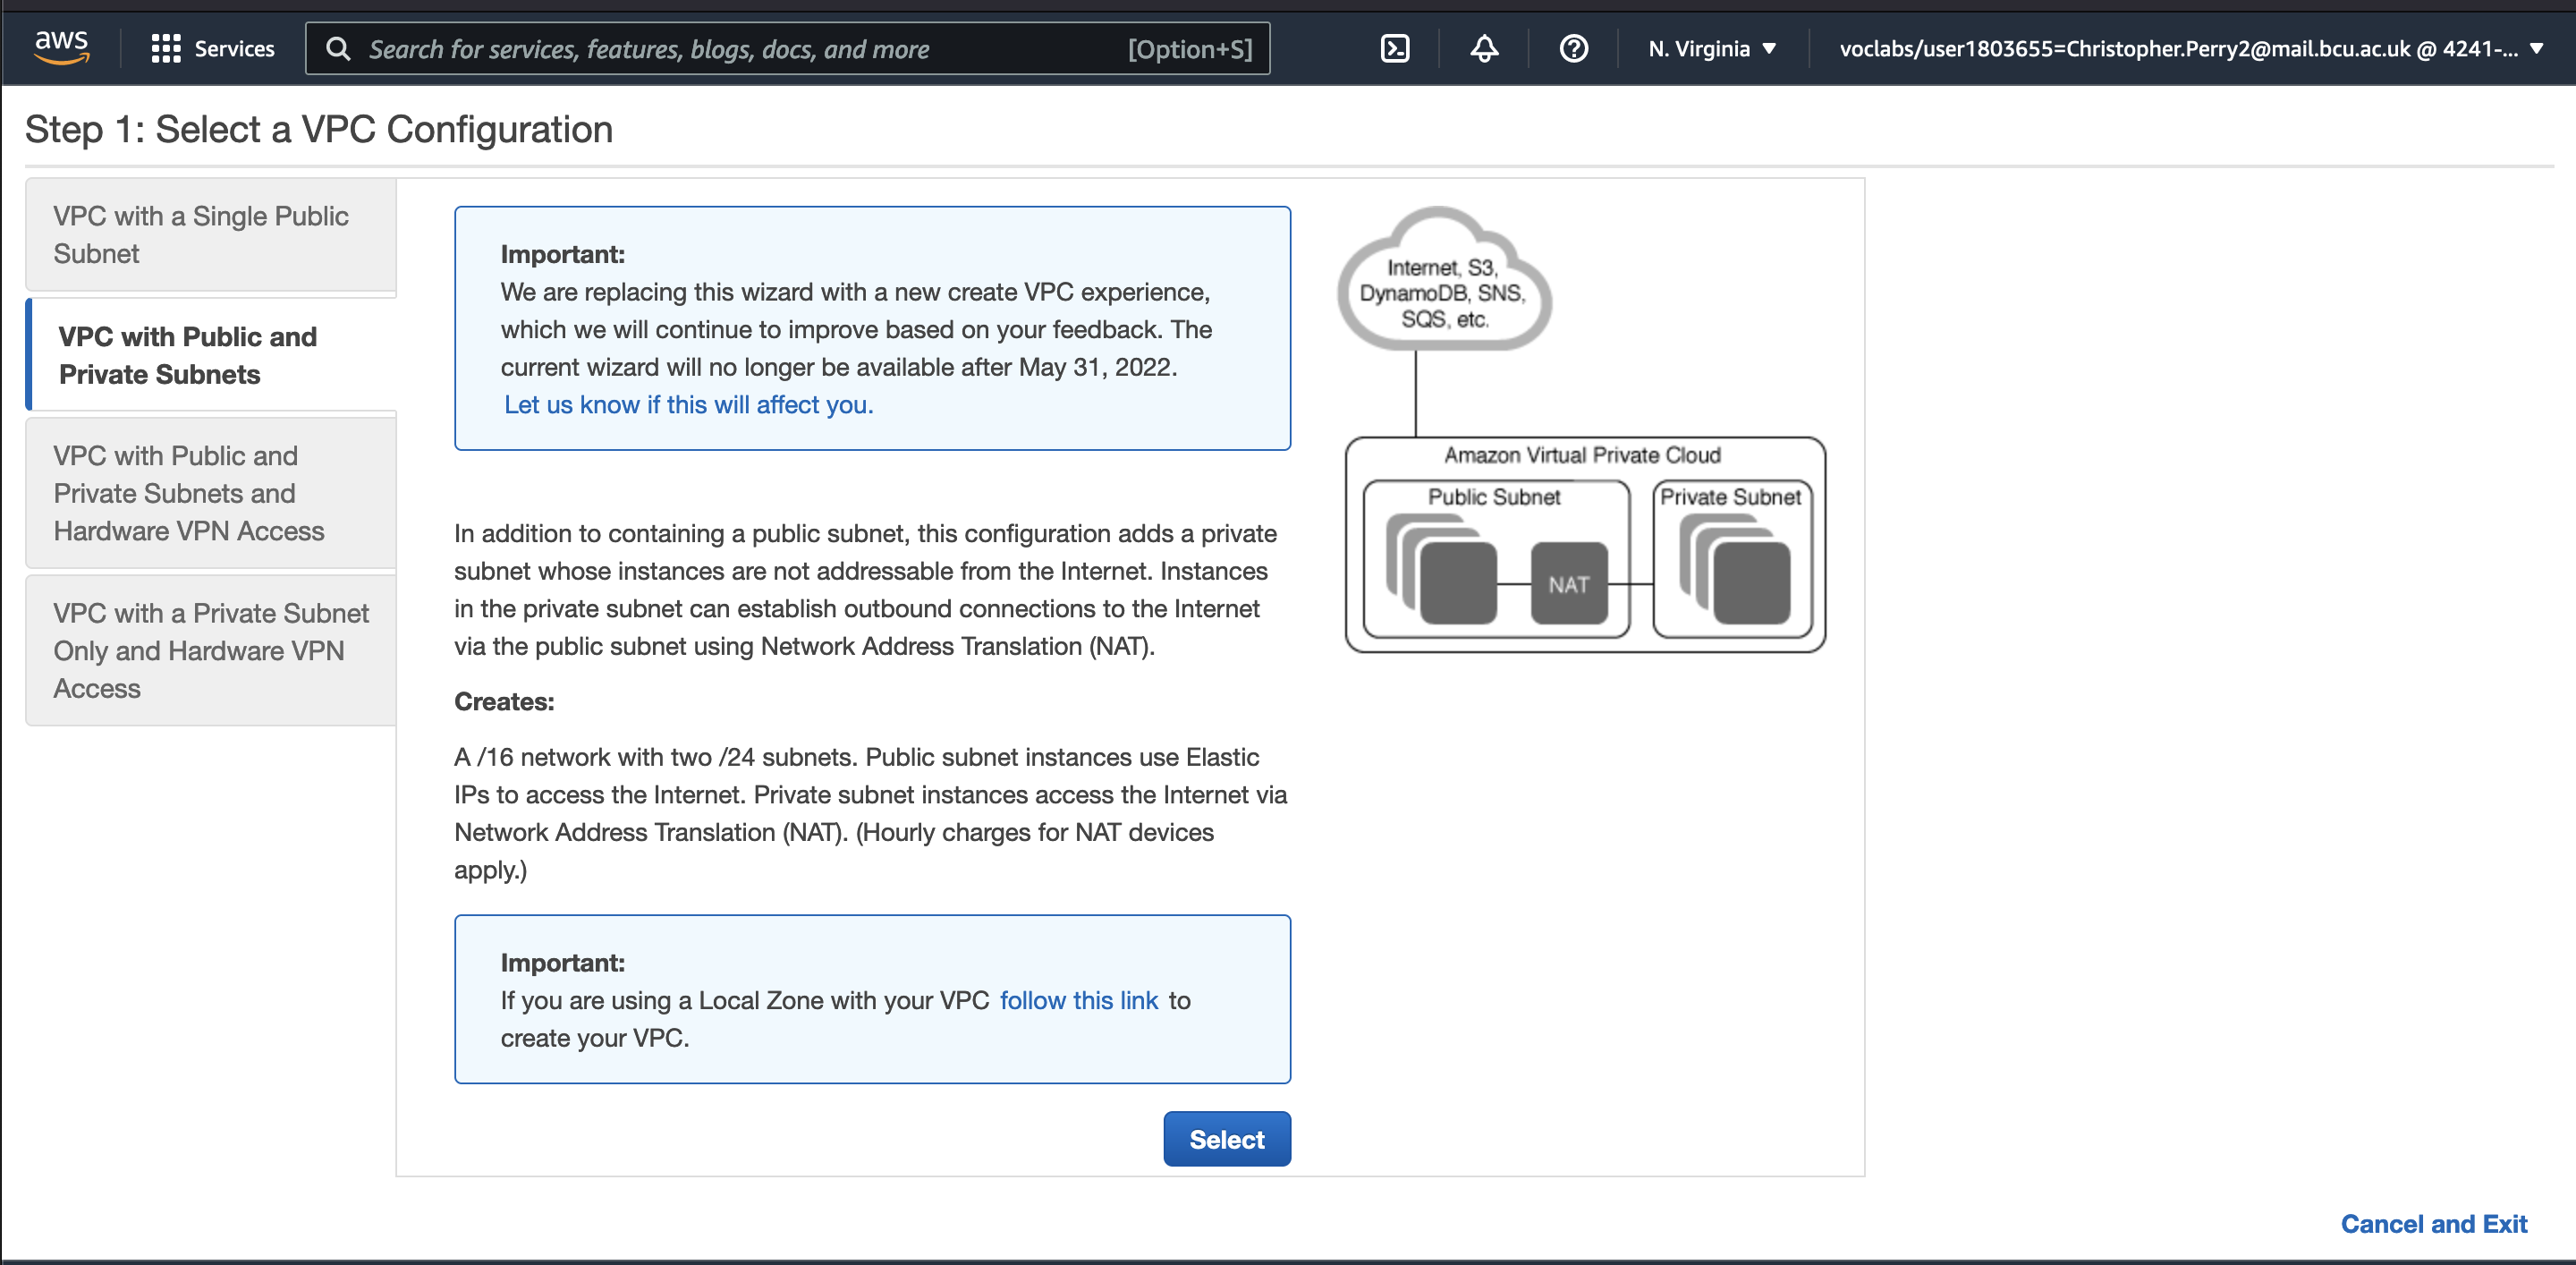
\includegraphics[width=\textwidth]{resources/selecting-a-vpc-configuration.png}
    \caption{Selecting a VPC Configuration}
    \label{fig:selecting-a-vpc-configuration}
\end{figure}

\begin{figure}[H]
    \centering
        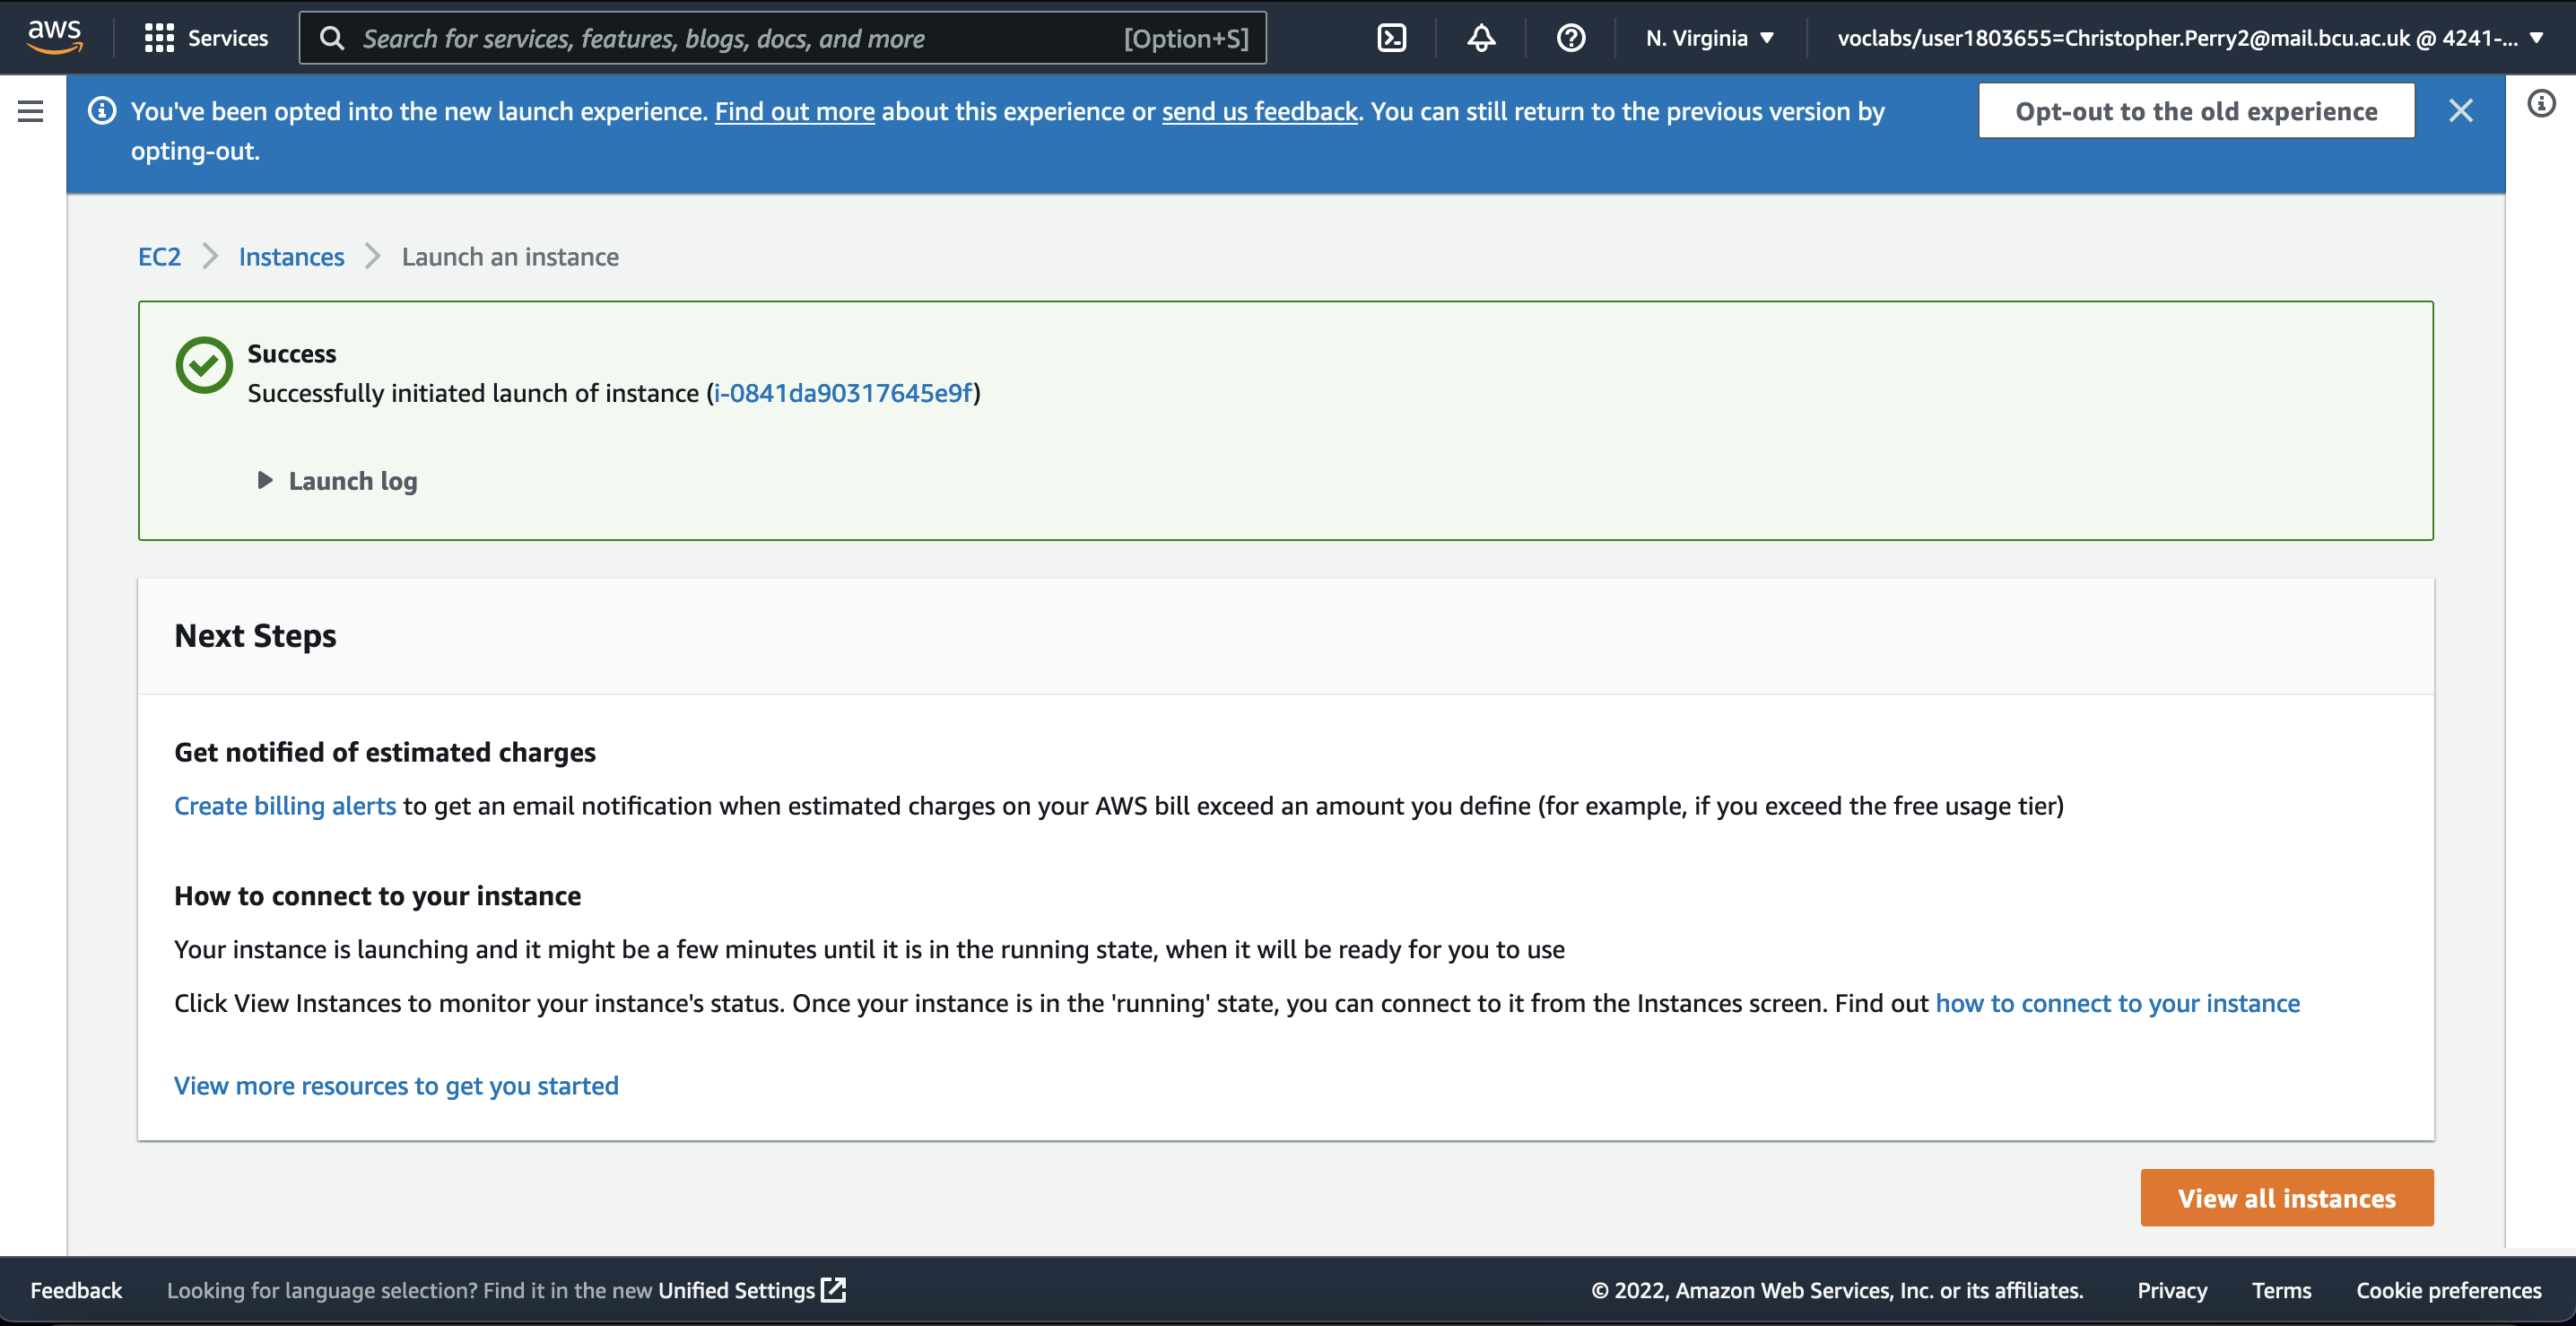
\includegraphics[width=\textwidth]{resources/successfully-initiated-instance.png}
    \caption{Successfully Initiated Instance}
    \label{fig:successfully-initiated-instance}
\end{figure}

\begin{figure}[H]
    \centering
        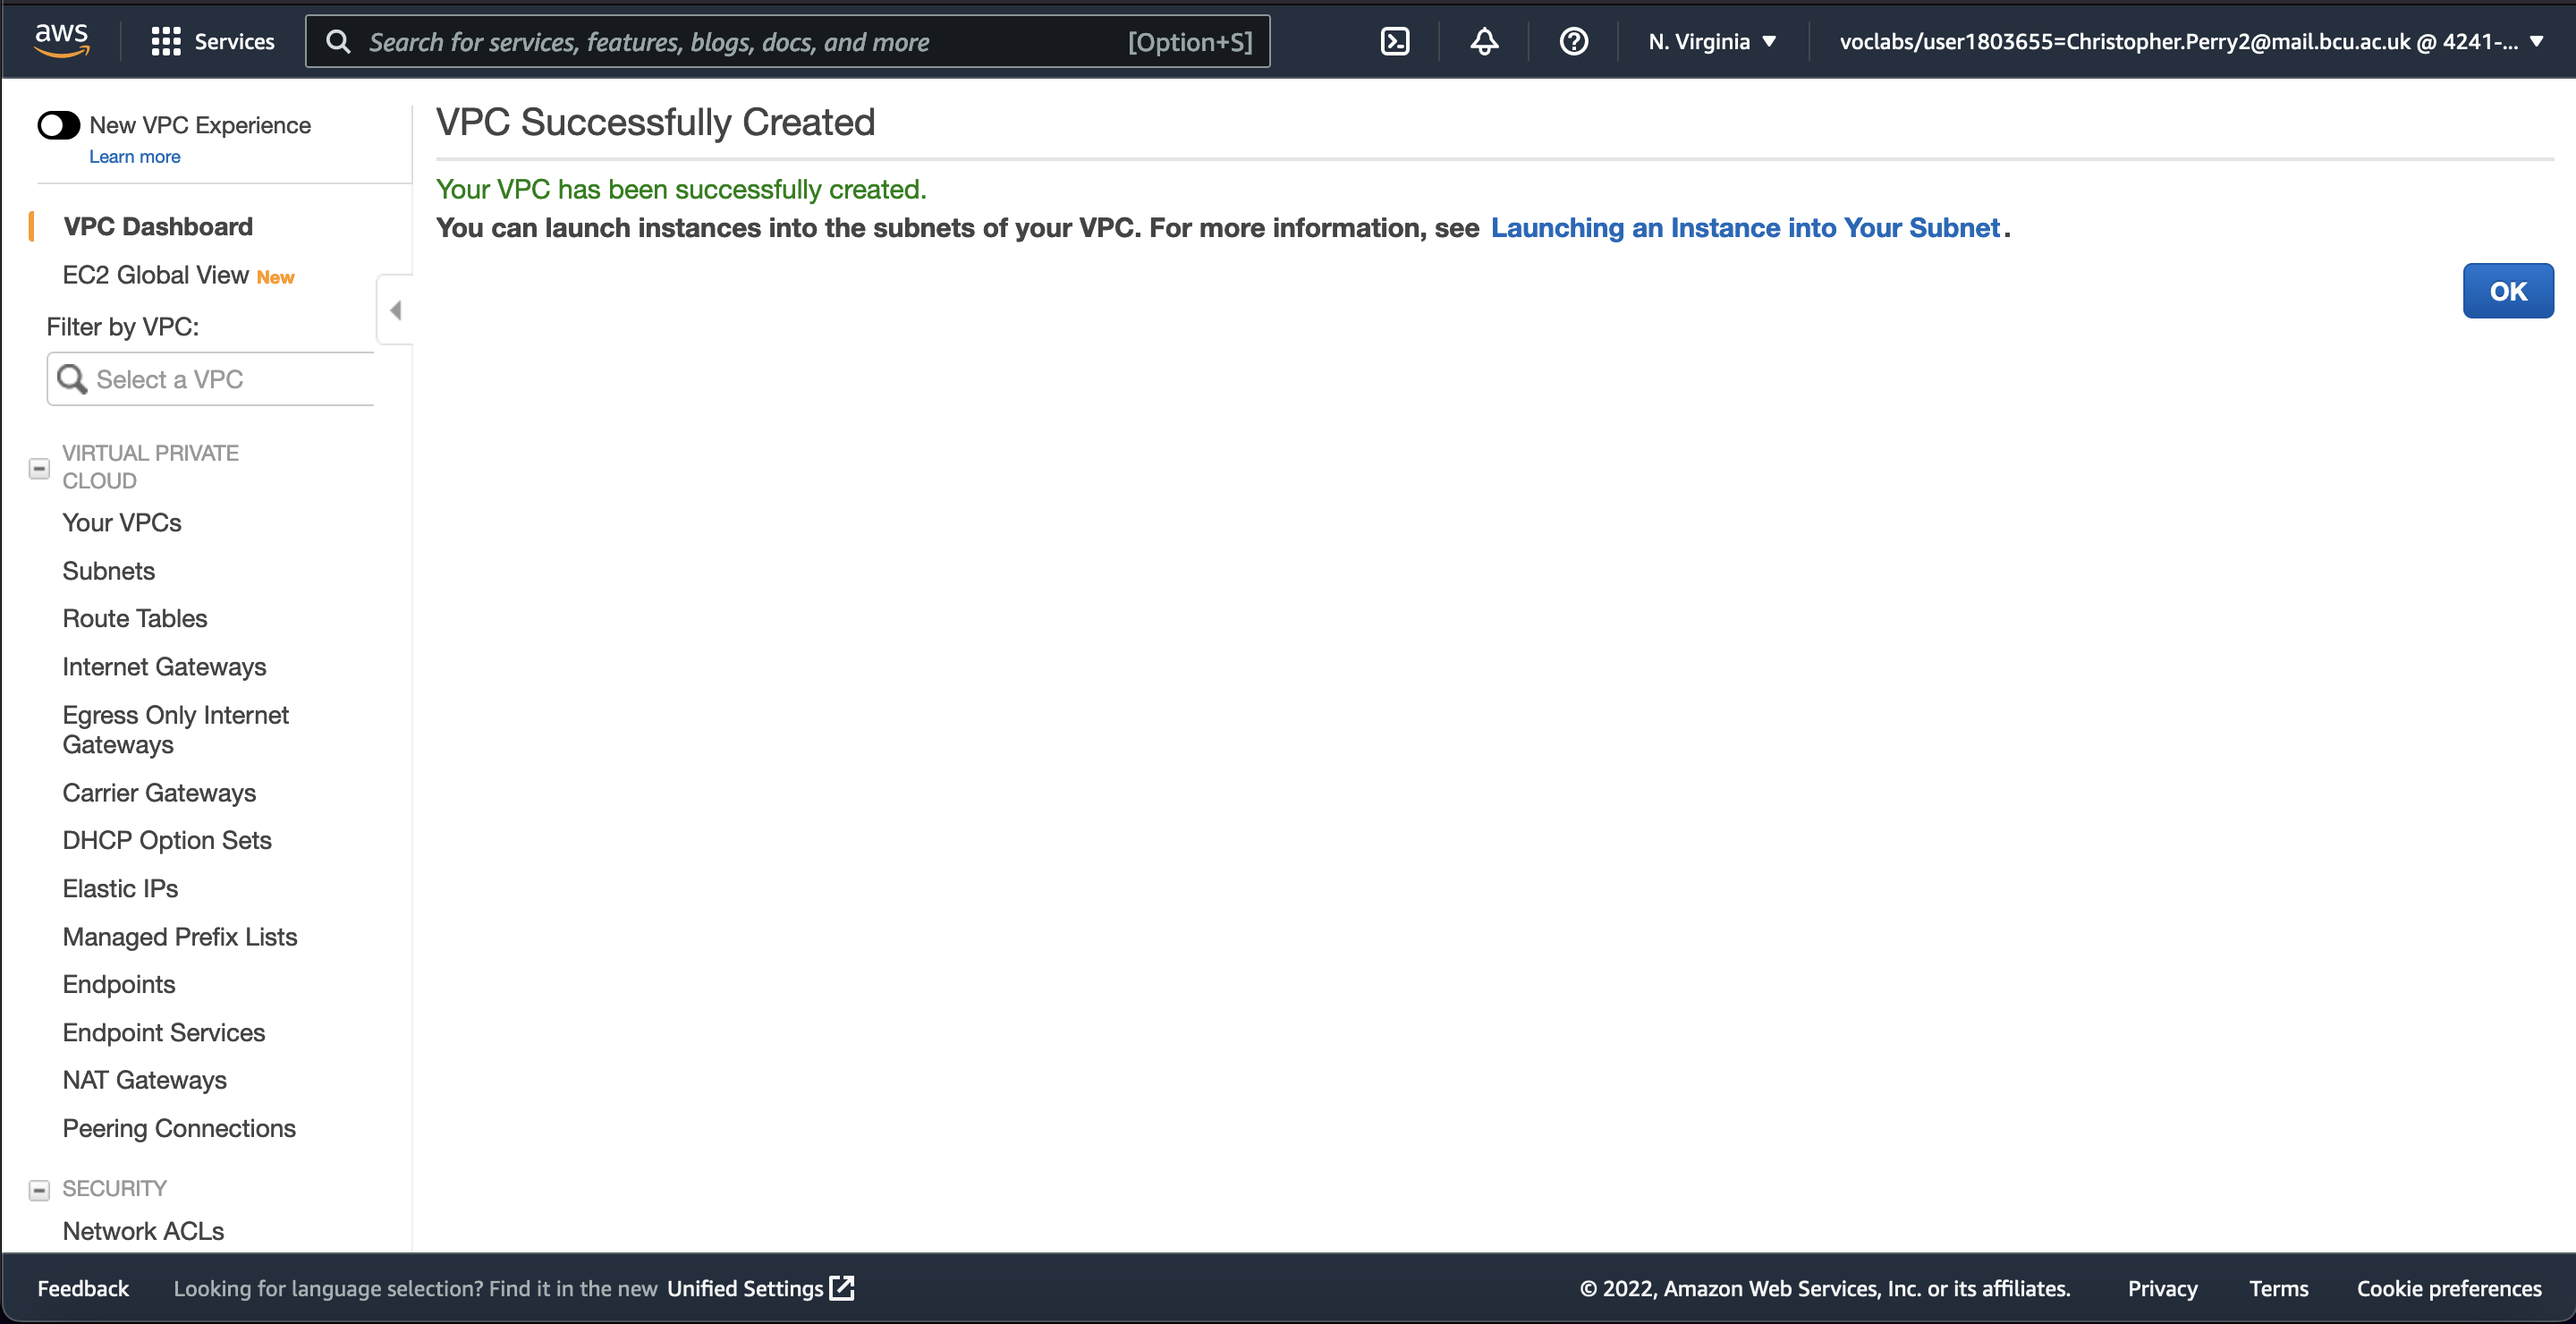
\includegraphics[width=\textwidth]{resources/vpc-successfully-created.png}
    \caption{VPC Successfully Created}
    \label{fig:vpc-successfully-created}
\end{figure}

\begin{figure}[H]
    \centering
        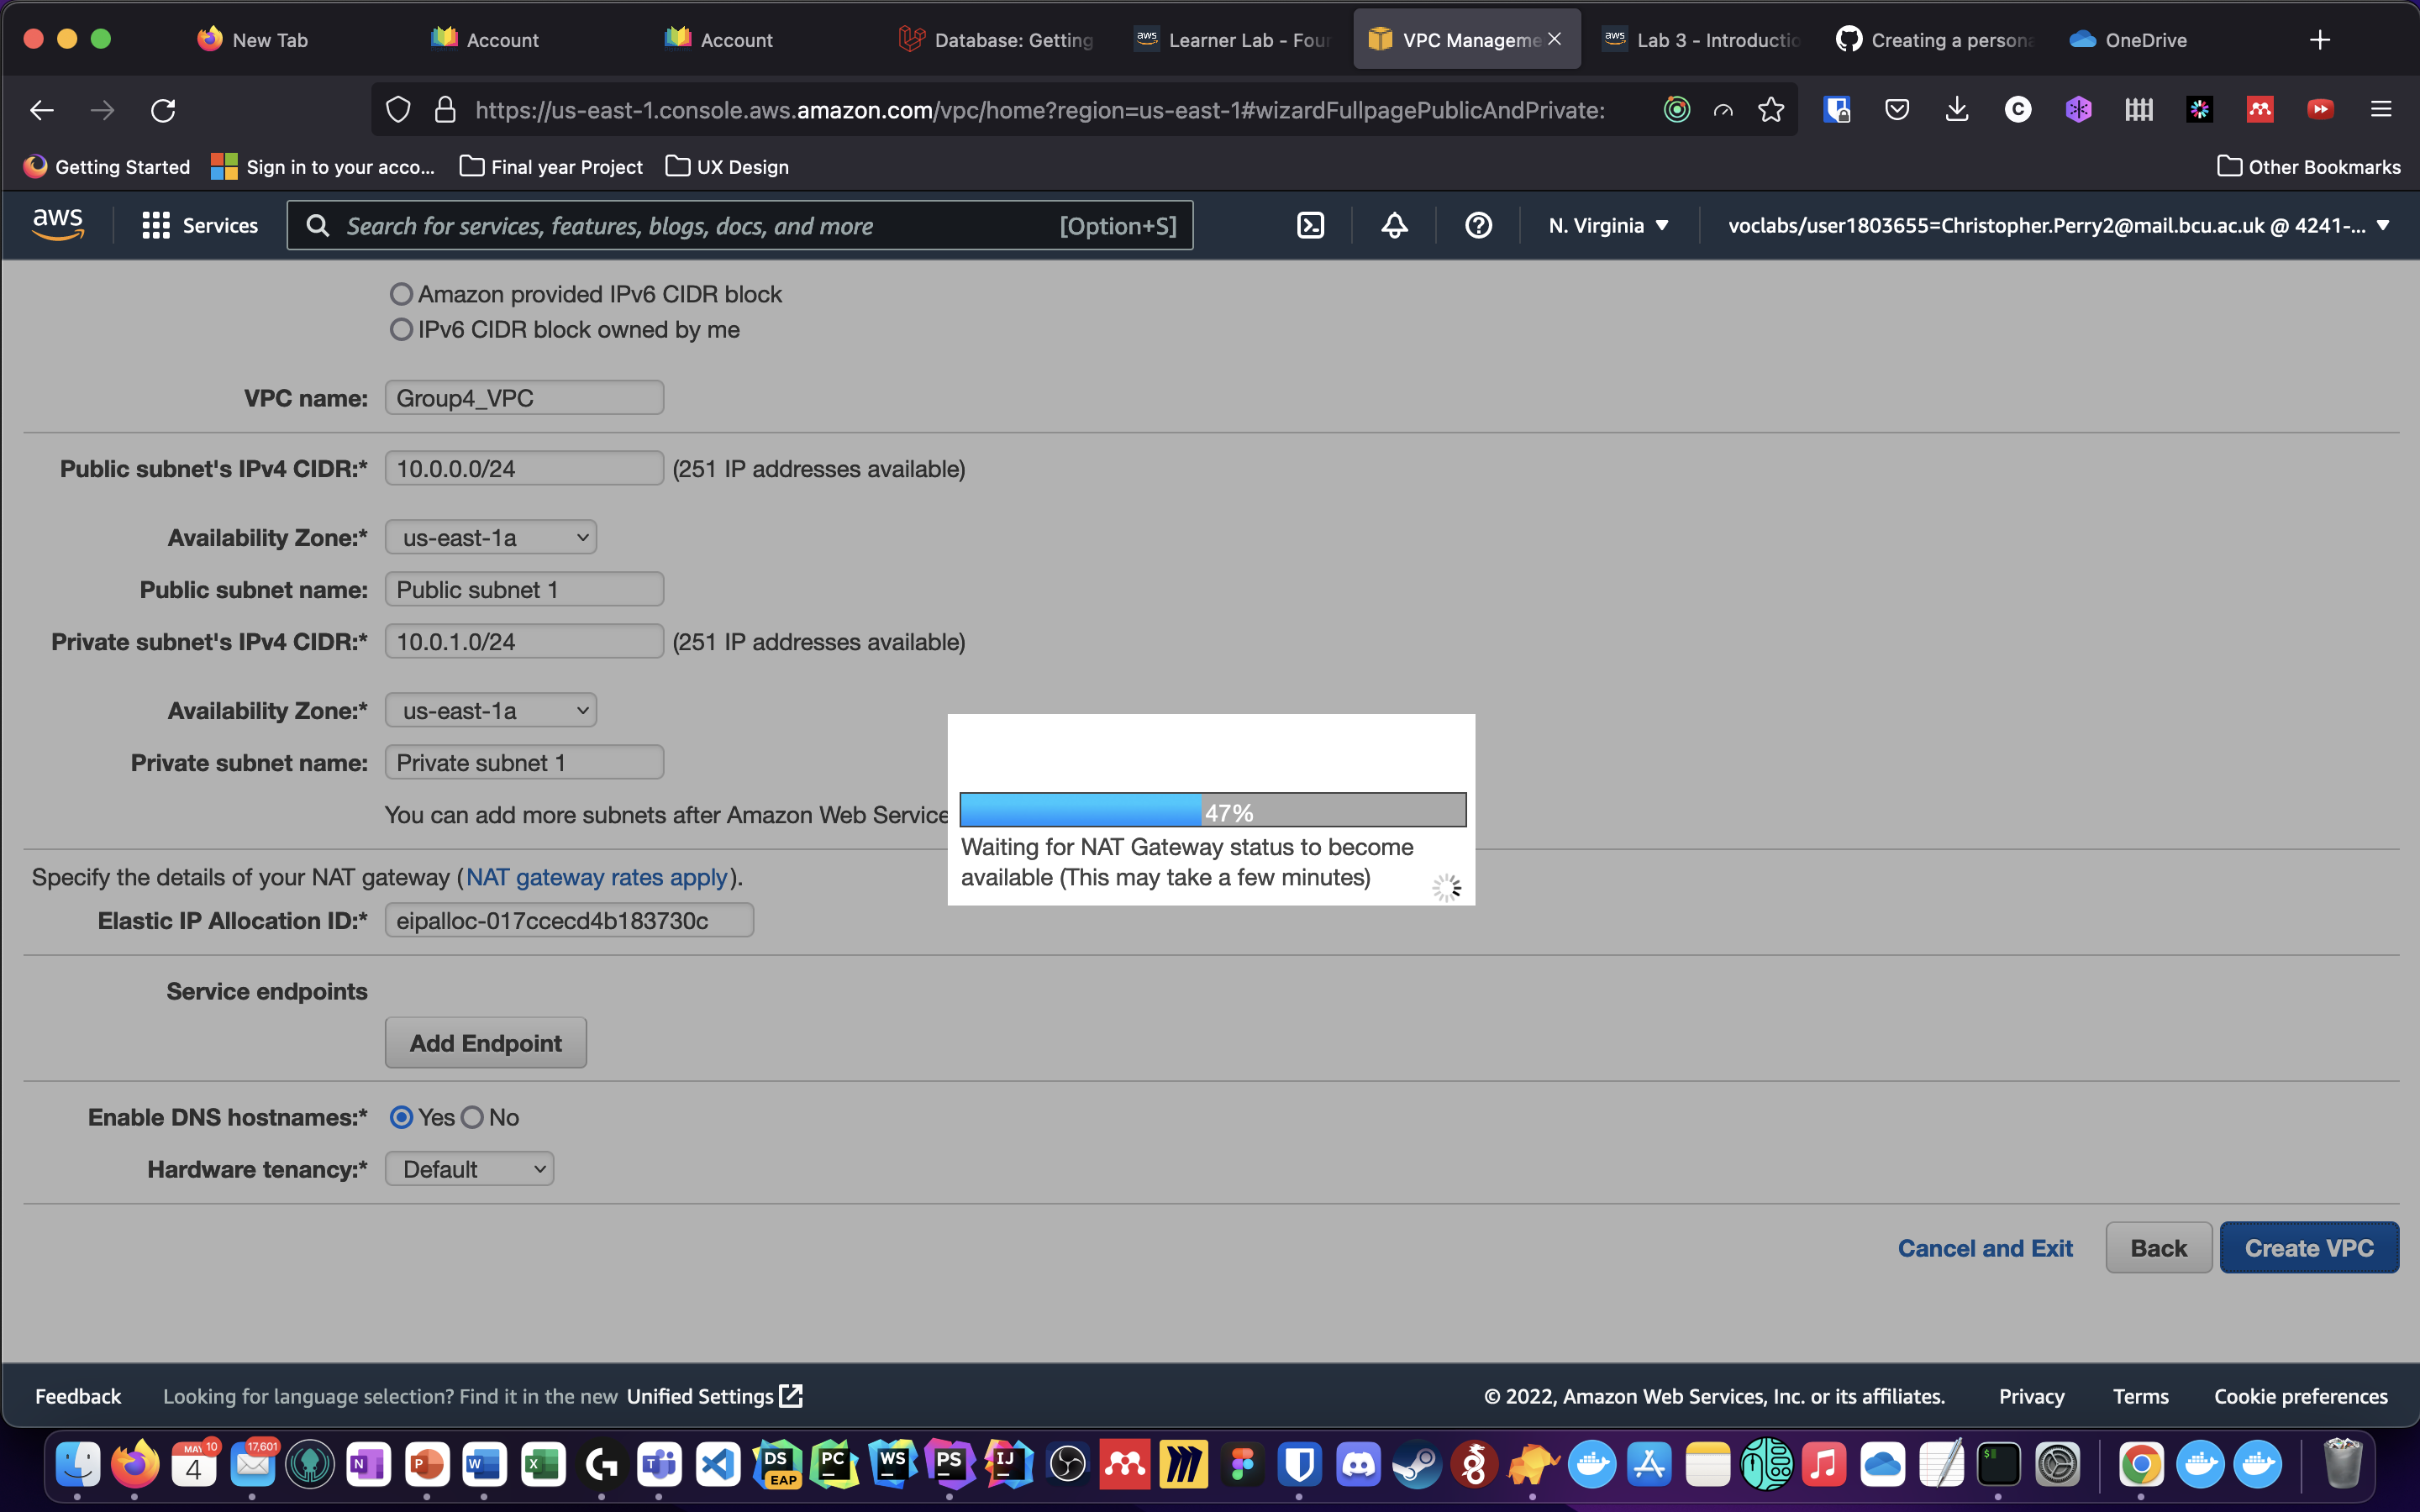
\includegraphics[width=\textwidth]{resources/vpc-with-public-and-private-subnets-loading.png}
    \caption{VPC with Public and Private Subnets, Loading}
    \label{fig:vpc-with-public-and-private-subnets-loading}
\end{figure}

\begin{figure}[H]
    \centering
        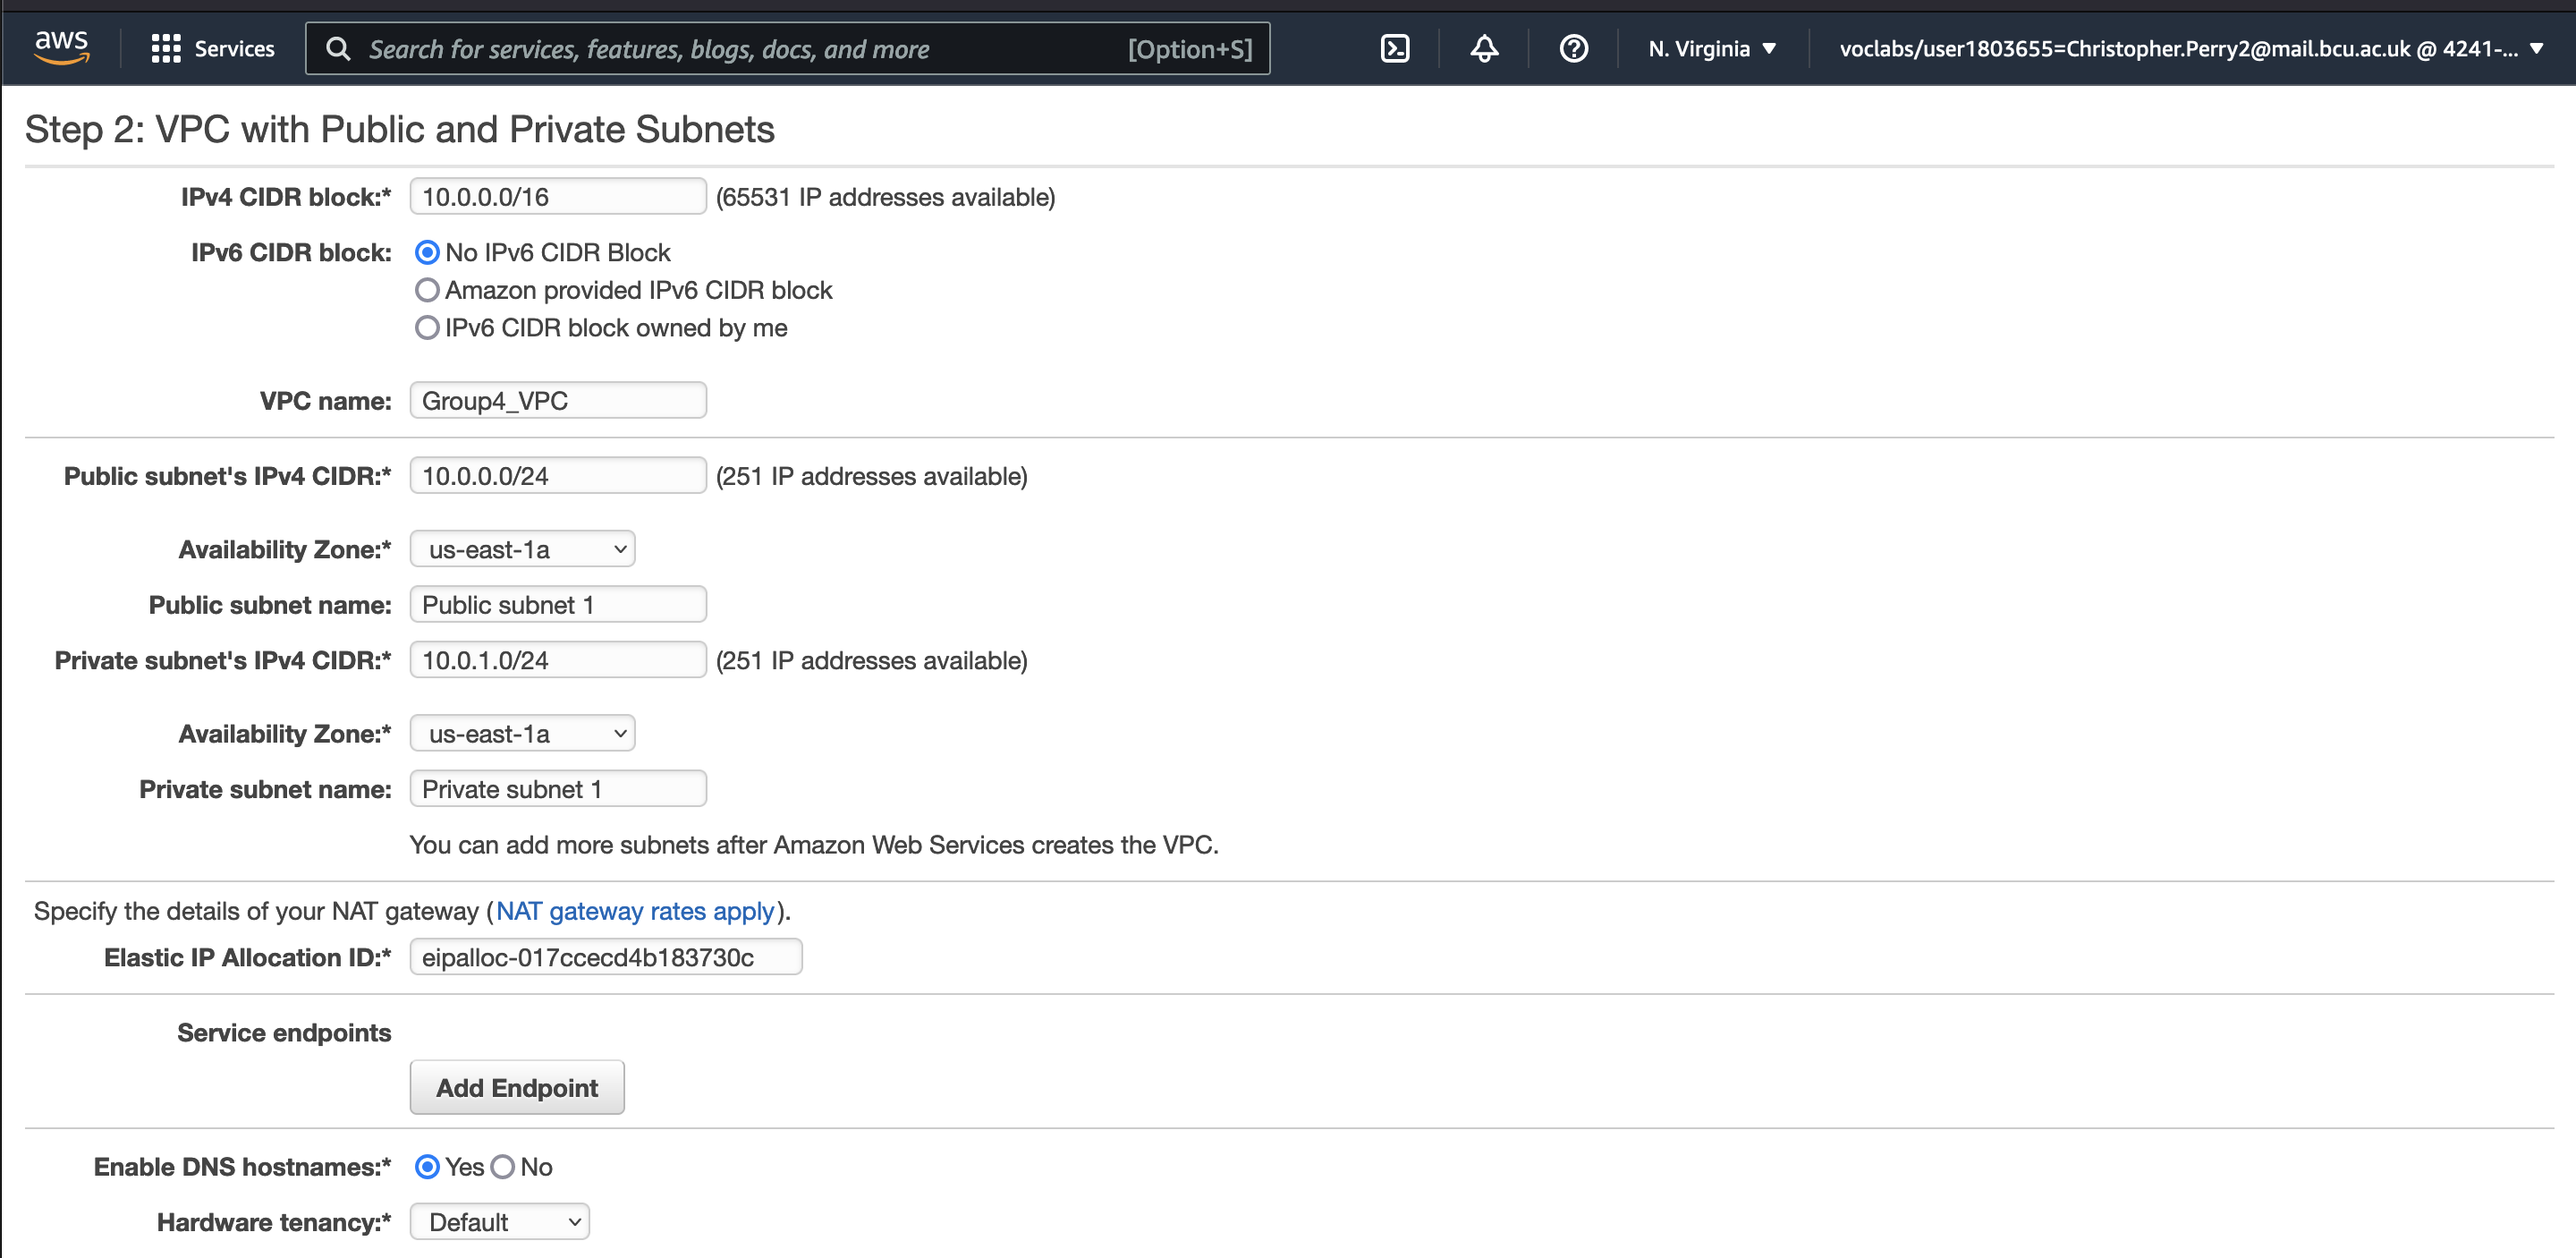
\includegraphics[width=\textwidth]{resources/vpc-with-public-and-private-subnets.png}
    \caption{VPC with Public and Private Subnets}
    \label{fig:vpc-with-public-and-private-subnets}
\end{figure}

\begin{figure}[H]
    \centering
        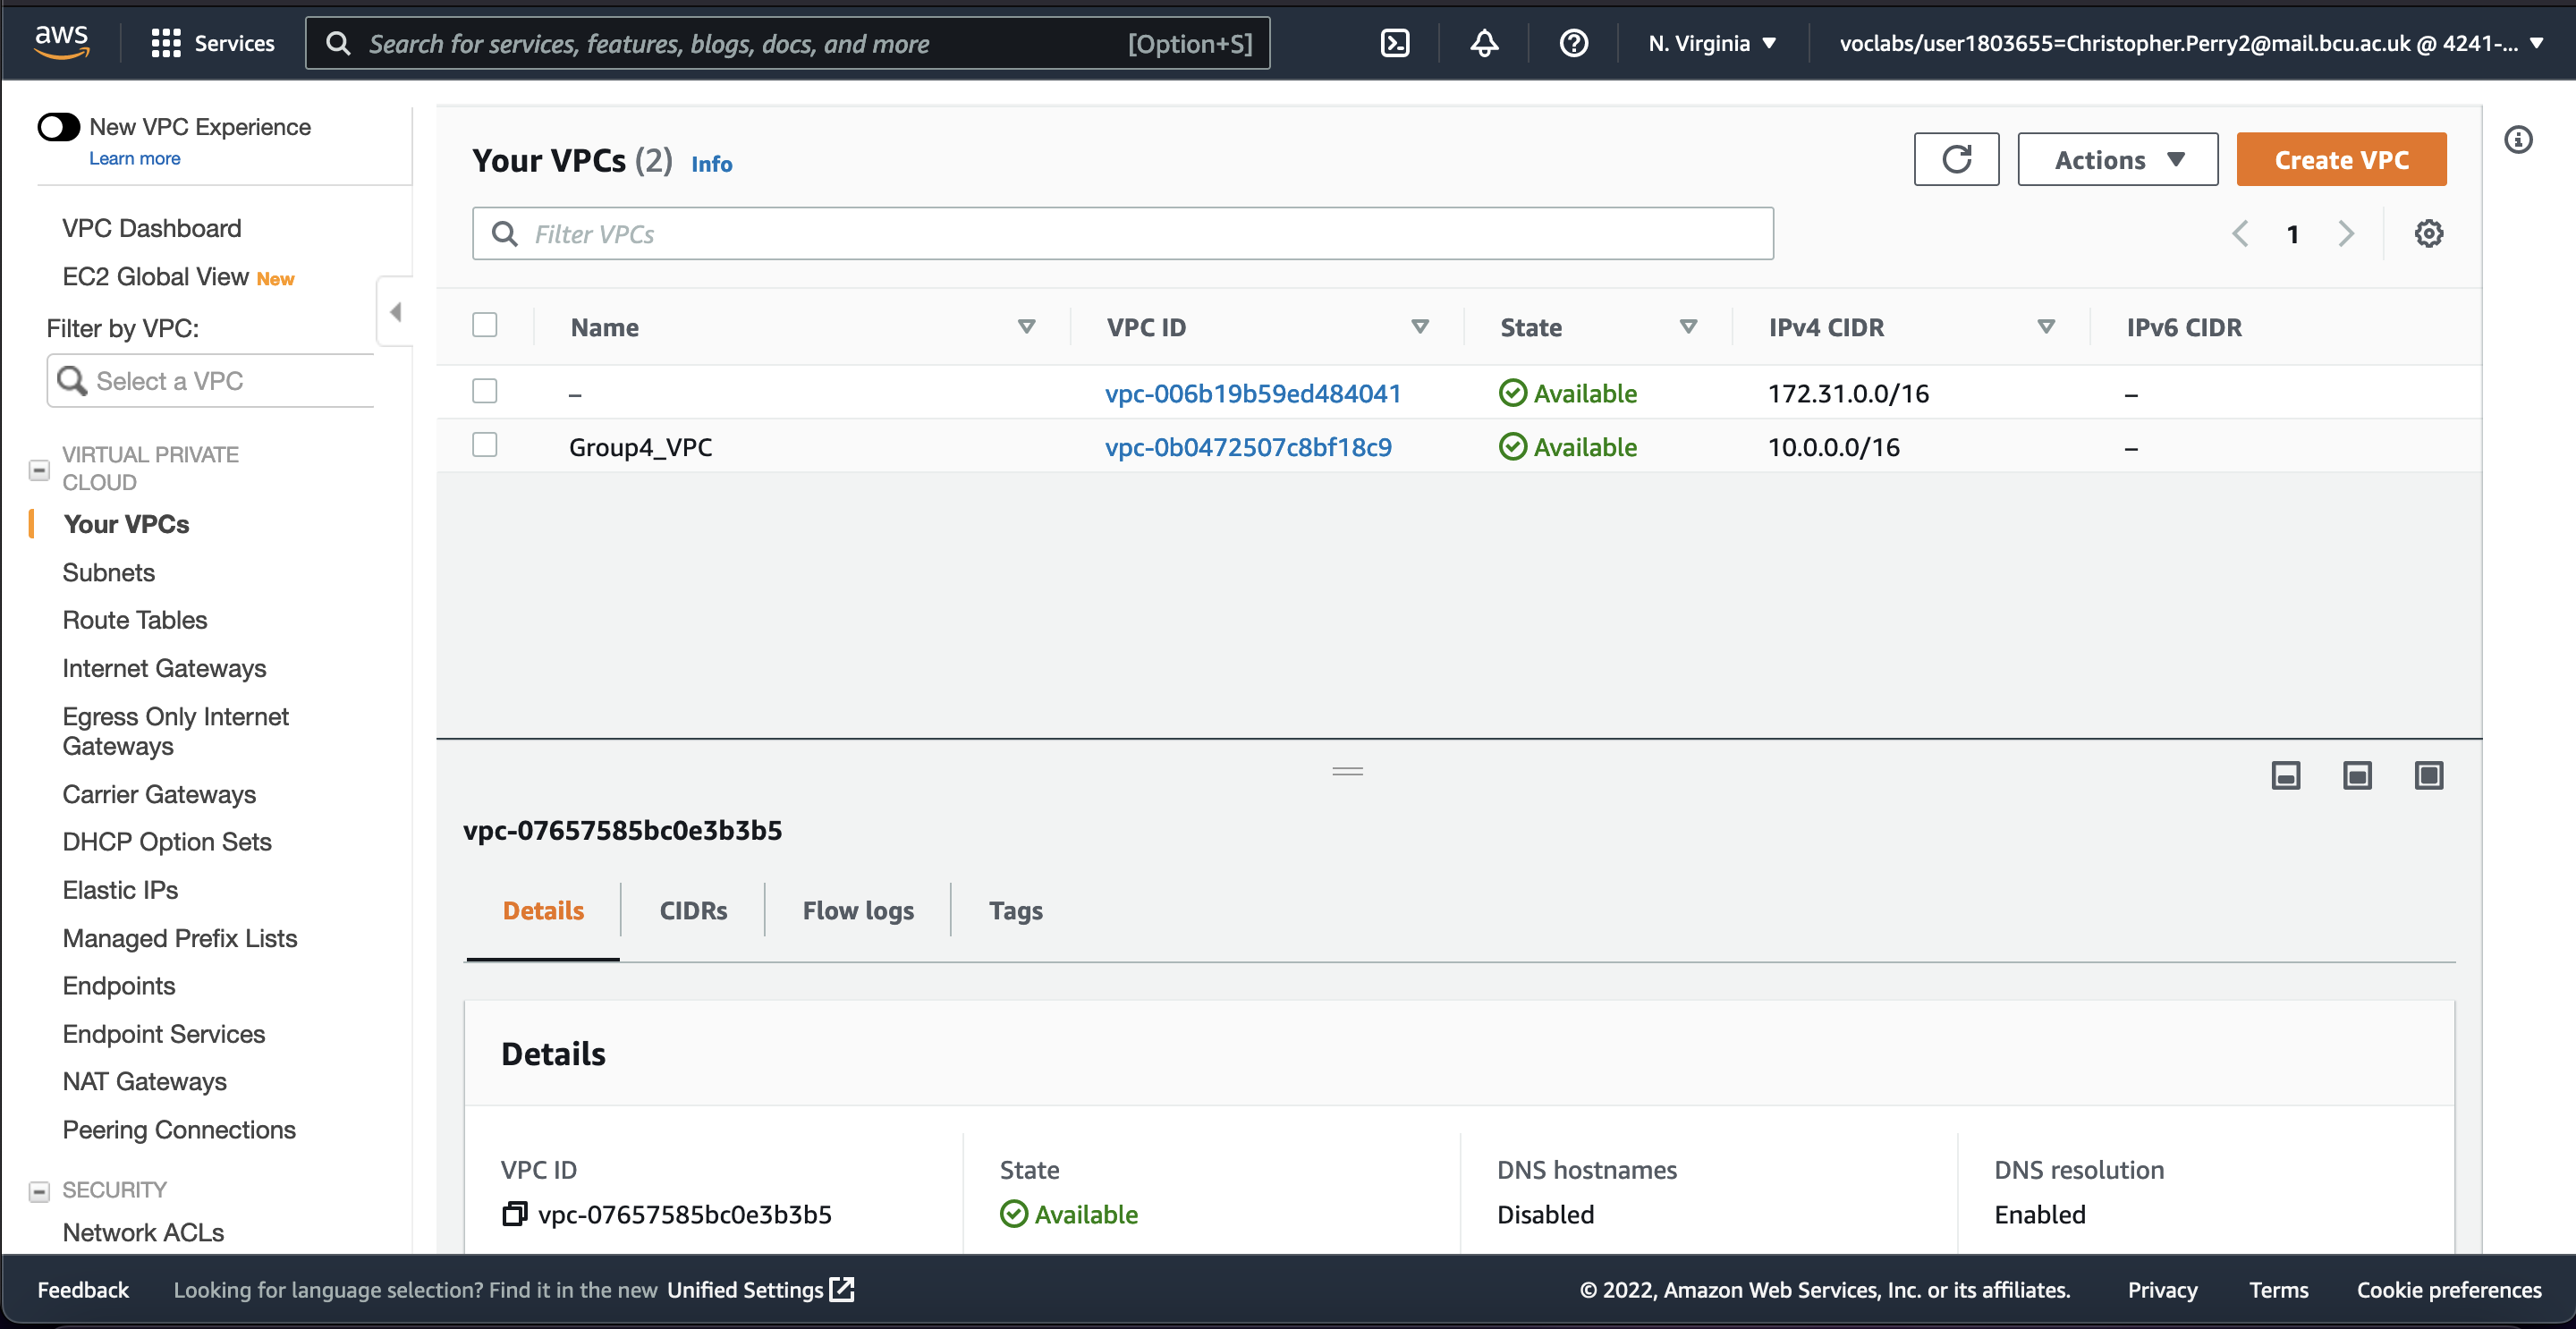
\includegraphics[width=\textwidth]{resources/your-vpcs.png}
    \caption{Your VPCs}
    \label{fig:your-vpcs}
\end{figure}